\documentclass{article}[12pt]
\usepackage{fancyhdr, fancybox, tabularx, verbatim, epsfig}
%\usepackage{fancyhdr, graphicx, fancybox, wrapfig, epic, ecltree, tabularx,
%  verbatim, alltt, ifthen, boxedminipage, epsfig}

\includeonly{overview, high_level, data_formats, data_interface, examples,
  advanced, functions, matrix_free}

%\setlength{\oddsidemargin}{0.4\oddsidemargin}
%\setlength{\evensidemargin}{0.4\evensidemargin}
%\setlength{\topmargin}{0.0\topmargin}
%\setlength{\textheight}{1.16\textheight}
%\setlength{\textwidth}{1.29\textwidth}
\setlength{\oddsidemargin}{0.3\oddsidemargin}
\setlength{\evensidemargin}{0.3\evensidemargin}
\setlength{\topmargin}{0.0\topmargin}
\setlength{\textheight}{1.16\textheight}
\setlength{\textwidth}{1.39\textwidth}

%
% macros for formatting symbols for reals, integers, etc.
%

\newcommand{\Az}  {{\bf Aztec}}
\newcommand\R     {{\rm \bf R}}
\newcommand\I     {{\rm \bf I}}
\newcommand\C     {{\rm \bf C}}

%
% define boxes for describing variables, etc
%

\def\optionbox#1#2{\noindent$\hphantom{hix}${\parbox[t]{2.10in}{\it
#1}}{\parbox[t]{3.9in}{#2}} \\[1.1em]}

\def\choicebox#1#2{\noindent$\hphantom{hixthere}$\parbox[t]{2.10in}{\sf
#1}\parbox[t]{3.5in}{#2}\\[0.8em]}

\def\structbox#1#2{\noindent$\hphantom{hix}${\parbox[t]{2.10in}{\it
#1}}{\parbox[t]{3.9in}{#2}} \\[.02cm]}

\def\in{\hskip .2in \=}
\def\hsp{\hskip .4in \=}
\def\sp{\hskip .18in \=}
\def\sh{\hskip .18in }
\def\bb{\hskip .034in }
\def\lil{\hskip .1in }


\def\protobox#1{\vspace{2em}{\flushleft{\bf Prototype}
\hrulefill}\flushleft{\fbox{\parbox[t]{6in}{\vspace{1em}{\sf
#1}\vspace{1em}}}}}

%--- redefine this for the tabularx environment

\newcolumntype{Y}{>{\raggedright\arraybackslash}X}
\newcolumntype{Z}{>{\small\raggedright\arraybackslash}X}

%
% ***********************************************************************
% * 02 July 1993: McCorkle                                              *
% * Define a macro that will lightly print the word `DRAFT' diagonally  *
% * across each page of the document. This macro was obtained from the  *
% * NMSU math department                                                *
% *                                                                     *
% * Usage: \draft                                                       *
% ***********************************************************************
%
\def\draft{%
\special{!userdict begin /bop-hook{gsave
200 30 translate 65 rotate
/Times-Roman findfont 216 scalefont setfont
0 0 moveto 0.9 setgray (DRAFT) show grestore}def end}
}

\renewcommand\baselinestretch{0.9}

\begin{document}

\large
\pagenumbering{roman}

%\draft                                   % Lightly print `DRAFT' on every
                                         % page of the document

%
% Stuff for SAND report style from B.A. Hendrickson, SNL, 1422
%
\hspace{2.22in}
SAND99--8801J
\hfill
Distribution

\hspace{2.07in}
Unlimited Release
\hfill
Category UC--405
\begin{center}
Printed Nov 1999
\end{center}

\vspace{0.8in}

\begin{center}
%{\Large{\bf \Az{} User's Guide$^\ast$ \\ Version 2.1}}
  {\Large{\bf Official \Az{} User's Guide\footnote{This work was supported by 
	the
        Applied Mathematical Sciences program, U.S. Department of Energy,
        Office of Energy Research, and was performed at Sandia National
        Laboratories, operated for the U.S. Department of Energy under contract
        No. DE-AC04-94AL85000. The \Az{} software package was developed by the
        authors at Sandia National Laboratories and is under copyright
        protection} \\ Version 2.1}}

\vspace*{0.4in}

Ray S. Tuminaro\footnote{Applied \& Numerical Mathematics Department;
  tuminaro@cs.sandia.gov; (925) 294-2564}
\,\,\,\,Mike Heroux\footnote{Applied \& Numerical Mathematics Department;
  maherou@cs.sandia.gov; (320) 845-7695}
\,\,\,\,Scott A. Hutchinson\footnote{Parallel Computational Sciences Department;
  sahutch@cs.sandia.gov; (505) 845-7996}
\,\,\,\, John N. Shadid\footnote{Parallel Computational Sciences Department;
  jnshadi@cs.sandia.gov; (505) 845-7876}
\\

Massively Parallel Computing Research Laboratory \\
Sandia National Laboratories \\
Albuquerque, NM \, 87185

\vspace*{.9in}

\end{center}

{\centering\large Abstract \\[1em]}

\Az{} is an iterative library that greatly simplifies the parallelization
process when solving the linear systems of equations $Ax = b$ where $A$ is a
user supplied $n \times n$ sparse matrix, $b$ is a user supplied vector of
length $n$ and $x$ is a vector of length $n$ to be computed. \Az{} is intended
as a software tool for users who want to avoid cumbersome parallel programming
details but who have large sparse linear systems which require an efficiently
utilized parallel processing system.  A collection of data transformation tools
are provided that allow for easy creation of distributed sparse unstructured
matrices for parallel solution. Once the distributed matrix is created,
computation can be performed on any of the parallel machines running \Az{}:
workstation clusters (DEC, SGI, SUN, LINUX, etc.), Cray T3E,
Intel TeraFlop, Intel Paragon, IBM SP2, nCUBE 2
as well as other
MPI platforms, vector machines or serial machines.

\Az{} includes a number of Krylov iterative methods such as conjugate gradient
(CG), generalized minimum residual (GMRES) and stabilized biconjugate gradient
(BiCGSTAB) to solve systems of equations.  These Krylov methods are used in
conjunction with various preconditioners such as polynomial or domain
decomposition methods using LU or incomplete LU factorizations within
subdomains. Although the matrix $A$ can be general, the package has been
designed for matrices arising from the approximation of partial differential
equations (PDEs).


\vfill

\newpage

%--- heading stuff

\pagestyle{fancyplain}
\addtolength{\headwidth}{\marginparsep}
%\addtolength{\headwidth}{\marginparwidth}
%--- remember section title
\renewcommand{\sectionmark}[1]{\markboth{#1}{}}
%\renewcommand{\subsectionmark}[1]{\markright{\thesubsection\ #1}}
%\lhead[\fancyplain{}{\bfseries\thepage}]%
%      {\fancyplain{}{\bfseries\rightmark}}
\rhead[\fancyplain{}{\bfseries\leftmark}]%
      {\fancyplain{}{\bfseries\thepage}}
\cfoot{}
%\rfoot{\leftmark\\\rightmark}

\large
\tableofcontents

\newpage

{\flushleft {\bf Notation Conventions} \hrulefill
\\[0.5em]

Different fonts are used to indicate program fragments, keys words, variables,
or parameters in order to clarify the presentation.  The table below describes
the meaning denoted by these different fonts.\\[3em]

\begin{tabularx}{\textwidth}{lX} \hline \\
{\bf Convention} & {\bf Meaning} \\[1.25em]

\tt typewriter & File names, code examples and code
fragments. \\

{\sf sans serif} & C language elements such as function names and constants
when they appear embedded in text or in function definition syntax
lines. \\

{\it italics\/} & Parameter and variable names when they appear embedded in
text or function definition syntax lines. \\

{\bf AZ\_ } & C language elements such as function names and constants which
are supplied by the \Az{} library. \\[1em] \hline
\end{tabularx}
%
\vskip 3.0em
\flushleft {\bf Code Distribution} \hrulefill
\\[0.5em]

\Az{} is publicly available for research purposes and may be licensed for
commercial application.  The code is distributed along with technical
documentation, example C and Fortran driver routines and sample input files via
the internet.  It may be obtained by contacting one of the authors listed on
page i of this report or from the \Az{} web site at
\tt http://www.cs.sandia.gov/CRF/aztec1.html.}

\newpage
\pagenumbering{arabic}

\section{Overview\label{overview}}
\Az{} is an iterative library that greatly simplifies the parallelization
process when solving the linear system of equations \[ Ax = b \] where $A$ is a
user supplied $n \times n$ sparse matrix, $b$ is a user supplied vector of
length $n$ and $x$ is a vector of length $n$ to be computed.  \Az{} is intended
as a software tool for users who want to avoid cumbersome parallel programming
details but who have large sparse linear systems requiring efficient use of a
parallel processing system.  The most complicated parallelization task for an
\Az{} user is the distributed matrix specification for the particular
application.  Although this may seem difficult, a collection of data
transformation tools are provided that allow creation of distributed sparse
unstructured matrices for parallel solution with ease of effort that is similar
to a serial implementation.  Background information regarding the data
transformation tools can be found in~\cite{aztec-utils}. Once the distributed
matrix is created, computation can occur on any of the parallel machines
running \Az{}: 
workstation clusters (DEC, SGI, SUN, LINUX, etc.), Cray T3E,  
Intel TeraFlop, Intel Paragon, IBM SP2, nCUBE 2 as well as other 
MPI platforms, vector machines or serial machines.

\Az{} includes a number of Krylov iterative methods such as conjugate gradient
(CG), generalized minimum residual (GMRES) and stabilized biconjugate gradient
(BiCGSTAB) to solve systems of equations.  These Krylov methods are used in
conjunction with various preconditioners such as polynomial preconditioners or
domain decomposition using LU or incomplete LU factorizations within
subdomains.  Background information concerning the iterative methods and the
preconditioners can be found in~\cite{aztec-alg}.  Although the matrix $A$ can
be general, the package has been designed for matrices arising from the
approximation of partial differential equations (PDEs). In particular, the
preconditioners, iterative methods and parallelization techniques are oriented
toward systems arising from PDE applications.  Lastly, \Az{} can work
with user-supplied matrix-vector product routines or two specific
sparse matrix formats 
(in which case \Az{} provides the matrix-vector product)
% and can perform incomplete factorizations)
-- a point-entry modified sparse row
(MSR) format or a block-entry variable block row (VBR) format.  These two
formats have been generalized for parallel implementation and, as such, are
referred to as ``distributed'' yielding DMSR and DVBR references.

The remainder of this guide describes how \Az{} is invoked within an
application.  \Az{} is written in ANSI-standard C and as such, all arrays in
the descriptions which follow begin indexing with 0.  Also, all function
prototypes (loosely, descriptions) are presented in ANSI C format.
Section~\ref{highlevel} discusses iterative method, preconditioning and
convergence options.  Section~\ref{data_formats} explains vectors and sparse
matrix formats supported by \Az{}.  In Section~\ref{highlevel_data_inter} we
discuss the data transformation tool for creating distributed vectors and
matrices. A concrete detailed programming example using this tool is given in
Section~\ref{examples} and some advance topics are discussed in
Section~\ref{advanced_topics}.  
Finally, 
Section~\ref{matrix.free} discusses Aztec's matrix-free interface and
Section~\ref{subroutines} gives a
glossary of \Az{} functions available to users.
% while in Section~\ref{comp_link} we discuss
%compiling and linking \Az{} on different systems with different
%applications.

%%% Local Variables:
%%% mode: latex
%%% TeX-master: "az_ug_20"
%%% End:


\section{{\protect \bf Aztec}: High Level View\label{highlevel}}

The following tasks must be performed to successfully
invoke \Az{}:
\begin{itemize}
\item describe the parallel machine (e.g. number of processors).
%      Done by invoking {\sf AZ\_set\_proc\_config} on the array
%      {\sf proc\_config} of size {\sf AZ\_PROC\_SIZE}.
\item initialize matrix and vector data structures.
\item choose iterative methods, preconditioners and the convergence criteria.
\item initialize the right hand side and initial guess.
\item invoke the solver.
\end{itemize}
A sample C program is shown in Figure~\ref{highlevel_code} omitting
declarations and some
%
\begin{figure}[Htbp]
  \shadowbox{
%    \begin{minipage}{\textwidth}
    \begin{minipage}{6.2in}
      \vspace{0.5em}
      {\large \flushleft{\bf Example}} \hrulefill %
      \vspace{0.5em}
%%%
\begin{verbatim}
#include "az_aztec.h"

void main(void) {

  AZ_set_proc_config(proc_config, AZ_NOT_MPI );

  init_matrix_vector_structures(bindx, val, update, external,
                                update_index, extern_index, data_org);

  AZ_defaults(options,params);
  choose_solver_options(options, params);

  init_guess_and_rhs(x, b, data_org, update, update_index);

  AZ_solve(x, b, options, params, bindx, val, data_org, status,
           proc_config);
}
\end{verbatim}
%%%
      \vspace{0.1em}
    \end{minipage}}
  \caption{High level code for \Az{} application.}\label{highlevel_code}
\end{figure}
%
parameters\footnote{The entire main program with specific sample problems is
  distributed with the package in the file \tt az\_main.c}. The functions
{\sf init\_matrix\_vector\_structures}, {\sf choose\_solver\_options}, and {\sf
  init\_guess\_and\_rhs} are supplied by the user.
All functions beginning with {\sf AZ\_} are \Az{} functions.
%and will be discussed in this document.
%The functions {\sf AZ\_set\_proc\_config} and {\sf
%AZ\_solve} are supplied with the library and are discussed in
%Section~\ref{subroutines}.
In this section, we give an overview of \Az{}'s features by describing the user
input arrays, {\it proc\_config}, {\it options\/} and {\it params\/}, that are set 
by the user.
A discussion of other parameters 
%{\sf init\_matrix\_vector\_structures} and {\sf init\_rhs\_guess}
is deferred to Sections~\ref{highlevel_data_inter} and~\ref{examples}.

\subsection{proc\_config\label{proc_configI}}
The integer array {\it proc\_config} of length {\sf AZ\_PROC\_SIZE}
is set by invoking {\sf AZ\_set\_proc\_config()}. This array
contains the number of processors, the processor id, and an MPI communicator
(if MPI is used\cite{mpi}). Most users need not be concerned with the
contents of this 
array. They must simply set it and pass it to other \Az{} functions.

\subsection{Aztec Options\label{optionI}}

The integer array {\it options\/} of length {\sf AZ\_OPTIONS\_SIZE} is set by 
the
user. It is used (but not altered) by the function {\sf AZ\_solve} to choose
between iterative solvers, preconditioners, etc.  Default values for
this array (as well as for {\it params}) are set by invoking 
{\sf AZ\_defaults()}.
Below we discuss each of the
possible options.  In some of these descriptions, reference is made to a
user-defined {\it options\/} or {\it params\/} value which is yet be
introduced.  These descriptions will follow but the reader may wish to ``jump
ahead'' and read the descriptions if the immediate context is not clear.

\vspace{2em}
{\flushleft{\bf Specifications} \hrulefill}
\nopagebreak \\[0.5em]
%
\optionbox{options[{\sf AZ\_solver}]}{Specifies solution
  algorithm. DEFAULT: \sf AZ\_gmres.}
\choicebox{AZ\_cg}{Conjugate gradient (only
  applicable to symmetric positive definite matrices).}
\choicebox{AZ\_gmres}{Restarted generalized minimal residual.}
\choicebox{AZ\_cgs}{Conjugate gradient squared.}
\choicebox{AZ\_tfqmr}{Transpose-free quasi-minimal residual.}
\choicebox{AZ\_bicgstab}{Bi-conjugate gradient with
  stabilization.}
\choicebox{AZ\_lu}{Sparse direct solver (single processor only).}
%
\optionbox{options[{\sf AZ\_scaling}]}{Specifies scaling algorithm.
  The entire matrix is scaled (overwriting the old
  matrix). Additionally, the right hand side, the initial guess and
  the final computed solution are scaled if necessary. For 
  symmetric scaling, this transforms $ A x = b$ into
  $ S A S y = S b $ as opposed to $ S A x = S b $ when symmetric
  scaling is not used. NOTE: The residual within \Az{} is now 
  given by $ S (b - A x) $. Thus, residual printing and convergence
  checking are effected by scaling.  DEFAULT: \sf
  AZ\_none.}
%
\choicebox{AZ\_none}{No scaling.}
\choicebox{AZ\_Jacobi}{Point Jacobi scaling.}
\choicebox{AZ\_BJacobi}{Block Jacobi scaling where the block
  size corresponds to the VBR blocks.  Point Jacobi scaling is
  performed when using the MSR format.}
\choicebox{AZ\_row\_sum}{Scale each row so the magnitude of its
  elements sum to 1.}
\choicebox{AZ\_sym\_diag}{Symmetric scaling so diagonal elements
  are 1.}
\choicebox{AZ\_sym\_row\_sum}{Symmetric scaling using the matrix
  row sums.}
%
\optionbox{options[{\sf AZ\_precond}]}{Specifies preconditioner.
  DEFAULT: \sf AZ\_none.}
\choicebox{AZ\_none}{No preconditioning.}
\choicebox{AZ\_Jacobi}{$k$ step Jacobi (block Jacobi for DVBR matrices
  where each block corresponds to a VBR block). The number of
  Jacobi steps, $k$, is set via {\it options}[{\sf AZ\_poly\_ord}].}
\choicebox{AZ\_Neumann}{Neumann series polynomial
  where the polynomial order is set via
  {\it options}[{\sf AZ\_poly\_ord}].}
\choicebox{AZ\_ls}{Least-squares polynomial
  where the polynomial order is set via
  {\it options}[{\sf AZ\_poly\_ord}].}
\choicebox{AZ\_sym\_GS}{Non-overlapping domain decomposition
  (additive Schwarz)
  $k$ step symmetric Gauss-Siedel.
  In particular, a symmetric Gauss-Siedel domain decomposition
  procedure is used where each processor independently
  performs one step of
  symmetric Gauss-Siedel on its local matrix, followed by communication
  to update boundary values before the next local symmetric
  Gauss-Siedel step. The number of steps, $k$, is set via
  {\it options}[{\sf AZ\_poly\_ord}].}
\choicebox{AZ\_dom\_decomp}{Domain decomposition preconditioner
  (additive Schwarz). That is, each processor augments
  its submatrix according to {\it options}[{\sf AZ\_overlap}]
  and approximately ``solves'' the resulting subsystem 
  using the solver specified by \\
  $\hphantom{using the solr}$
  {\it options}[{\sf AZ\_subdomain\_solve}].\\
  Note: {\it options}[{\sf AZ\_reorder}] determines whether
  matrix equations are reordered (RCM) before ``solving'' submatrix problem.}
\optionbox{options[{\sf AZ\_subdomain\_solve}]}{Specifies the solver
  to use on each subdomain when {\it options}[{\sf AZ\_precond}] is set
  to {\sf AZ\_dom\_decomp} DEFAULT: \sf AZ\_ilut.}
\choicebox{AZ\_lu}{Approximately solve processor's submatrix via
  a sparse LU factorization in conjunction with a drop tolerance 
  {\it params}[{\sf AZ\_drop}]. The current sparse
  lu factorization is provided by the package y12m~\cite{y12m}.}
\choicebox{AZ\_ilut}{Similar to {\sf AZ\_lu} using
  Saad's {\sf ILUT} instead of LU \cite{ilut}. The drop 
  tolerance is given by {\it params}[{\sf AZ\_drop}]
  while the fill-in is given by {\it params}[{\sf AZ\_ilut\_fill}]. }
\choicebox{AZ\_ilu}{Similar to {\sf AZ\_lu} using
  {\sf ilu(k)} instead of LU with k determined by 
  {\it options}[{\sf AZ\_graph\_fill}]}
\choicebox{AZ\_rilu}{Similar to {\sf AZ\_ilu} using
  {\sf rilu(k,$\omega$)} instead of {\sf ilu(k)}
  with $\omega$ ($0 \ge \omega \ge 1$) given by {\it params}[{\sf AZ\_omega}]
  \cite{milu}.}
\choicebox{AZ\_bilu}{Similar to {\sf AZ\_ilu} using block
  {\sf ilu(k)} instead of {\sf ilu(k)} where each block corresponds
  to a VBR block.}
\choicebox{AZ\_icc}{Similar to {\sf AZ\_ilu} using
  {\sf icc(k)} instead of {\sf ilu(k)} \cite{icc}.}
%
\optionbox{options[{\sf AZ\_conv}]}{Determines the residual expression used
  in convergence checks and printing.  DEFAULT: {\sf AZ\_r0}.
  The iterative solver terminates if the corresponding residual expression
  is less than {\it params}[{\sf AZ\_tol}]:}
\choicebox{AZ\_r0}{$\|r\|_2 / \|r^{(0)}\|_2 $}
\choicebox{AZ\_rhs}{$\|r\|_2 / \|b\|_2 $}
\choicebox{AZ\_Anorm}{$\|r\|_2 / \|A\|_{\infty} $}
\choicebox{AZ\_noscaled}{$\|r\|_2$}
\choicebox{AZ\_sol}{$\|r\|_{\infty}
  /(\|A\|_{\infty} * \|x\|_1 + \|b\|_{\infty}) $}
\choicebox{AZ\_weighted}{$\|r\|_{WRMS} $\\
  where $\| \cdot \|_{WRMS} = \sqrt{(1/n) \sum_{i=1}^n (r_i/w_i)^2}$,
  $n$ is the total number of unknowns, $w$ is a weight
  vector provided by the
  user  via {\it params}[{\sf AZ\_weights}] and
  $r^{(0)}$ is the initial residual.}
%
\optionbox{options[{\sf AZ\_output}]}{Specifies information (residual
  expressions - see {\it options}[{\sf AZ\_conv}]) to be printed.
  DEFAULT: \sf 1.}
\choicebox{AZ\_all}{Print out the matrix and indexing vectors for
  each processor. Print out all intermediate residual expressions.}
\choicebox{AZ\_none}{No intermediate results are printed.}
\choicebox{AZ\_warnings}{Only Aztec warnings are printed.}
\choicebox{AZ\_last}{Print out only the final residual expression.}
\choicebox{$>$ 0}{Print residual expression every {\it
    options[{\sf AZ\_output}]\/} iterations.}
%
\optionbox{options[{\sf AZ\_pre\_calc}]}{Indicates whether to use
  factorization information from previous calls to {\sf AZ\_solve}.
  DEFAULT: {\sf AZ\_calc}.}
\choicebox{AZ\_calc}{Use no information from previous {\sf
    AZ\_solve} calls.}
\choicebox{AZ\_recalc}{Use preprocessing information from a
  previous call but recalculate preconditioning factors. This is
  primarily intended for factorization software which performs a
  symbolic stage.}
\choicebox{AZ\_reuse}{Use preconditioner from a previous
  {\sf AZ\_solve} call, do not recalculate preconditioning factors.
  Also, use scaling factors from previous call to scale the
  right hand side, initial guess and the final solution.}
%
%
\optionbox{options[{\sf AZ\_graph\_fill}]}{The level of graph fill-in (k)
  for incomplete factorizations: ilu(k), icc(k), bilu(k).
  DEFAULT: 0}
%
\optionbox{options[{\sf AZ\_max\_iter}]}{Maximum number of iterations. DEFAULT:
  500.}
%
\optionbox{options[{\sf AZ\_poly\_ord}]}{The polynomial order when using
  polynomial preconditioning.  Also, the number of steps when using Jacobi or
  symmetric Gauss-Seidel preconditioning.  DEFAULT: 3.}
%
\optionbox{options[{\sf AZ\_overlap}]}{Determines the submatrices factored with
  the domain decomposition algorithms (see {\it options}[{\sf AZ\_precond}]).
  DEFAULT: 0.}
%
%\choicebox{AZ\_none}{Factor the local submatrix defined on this processor
%  by discarding column entries that correspond to external elements.}
%
\choicebox{AZ\_diag}{Factor the local submatrix defined on this processor
  augmented by a diagonal (block diagonal for VBR format) matrix. This diagonal
  matrix corresponds to the diagonal entries of the matrix rows (found on other
  processors) associated with external elements.  This can be viewed as taking
  one Jacobi step to update the external elements and then performing domain
  decomposition with {\sf AZ\_none} on the residual equations.}
%
\choicebox{k}{Augment each processor's local submatrix with
  rows from other processors. The new rows are obtained in k 
  steps (k $\ge$ 0). Specifically at each augmentation step,
  rows corresponding to external unknowns are obtained. These
  external unknowns are defined by nonzero columns in the 
  current augmented matrix not containing a corresponding
  row on this processor. After the k steps, all columns 
  associated with external
  unknowns are discarded to obtain a square matrix.
  The resulting procedure is an overlapped additive Schwarz
  procedure.}
%
\optionbox{options[{\sf AZ\_type\_overlap}]}{Determines how overlapping
    subdomain results are combined when different processors
    have computed different values for the same unknown.
    DEFAULT: \sf AZ\_standard.}
\choicebox{AZ\_standard}{The resulting value of an unknown is 
    determined by the processor owning that unknown. Information
    from other processors about that unknown is discarded.}
\choicebox{AZ\_symmetric}{Add together the results obtained from different
    processors corresponding to the same unknown. This keeps the 
    preconditioner symmetric if a symmetric technique was used on
    each subdomain.}
%
\optionbox{options[{\sf AZ\_kspace}]}{Krylov subspace size for
  restarted GMRES.\\
  DEFAULT: 30.}
%
\optionbox{options[{\sf AZ\_reorder}]}{Determines whether RCM reordering
  will be done in conjunction with domain decomposition incomplete 
  factorizations. 1 indicates RCM reordering is used. 0 indicates that
  equations are not reordered.  DEFAULT:~1.}
%
\optionbox{options[{\sf AZ\_keep\_info}]}{Determines whether matrix
  factorization information will be kept after this solve (for example
  to solve the same system with another right hand side, see 
  {\it options}[{\sf AZ\_pre\_calc}]).  1 indicates factorization 
  information is kept.  0 indicates that factorization information is
  discarded.  DEFAULT: 0.}
%
\optionbox{options[{\sf AZ\_orthog}]}{GMRES orthogonalization scheme.\\
  DEFAULT: {\sf AZ\_classic}.}
\choicebox{AZ\_classic}{2 steps of classical Gram-Schmidt orthogonalization.}
\choicebox{AZ\_modified}{Modified Gram-Schmidt orthogonalization.}
%
\optionbox{options[{\sf AZ\_aux\_vec}]}{Determines $\tilde r$ (a required
  vector within some iterative methods). The convergence behavior varies
  slightly depending on how this is set.  DEFAULT: \sf AZ\_resid.}
\choicebox{AZ\_resid}{$\tilde r$ is set to the initial residual vector.}
\choicebox{AZ\_rand}{$\tilde r$ is set to random numbers between -1 and 1.
  NOTE: When using this option, the convergence depends on the number of
  processors (i.e. the iterates obtained with x processors differ from the
  iterates obtained with y processors if x $\ne$ y).}  $\hphantom{h}$
\subsection{\Az{} parameters\label{optionD}}

The double precision array {\it params\/} set by the user and normally of
length {\sf AZ\_PARAMS\_SIZE}. However, when a weight vector is needed for the
convergence check (i.e. {\it options}[{\sf AZ\_conv}] = {\sf AZ\_weighted}), it
is embedded in {\it params\/} whose length must now be {\sf AZ\_PARAMS\_SIZE} +
\# of elements updated on this processor.  In either case, the contents of {\it
  params\/} are used (but not altered) by the function {\sf AZ\_solve} to
control the behavior of the iterative methods.  The array elements are
specified as follows: \vspace{2em}
{\flushleft{\bf Specifications} \hrulefill} \nopagebreak \\[0.5em]
%
\optionbox{params[{\sf AZ\_tol}]}{Specifies tolerance value used in
   conjunction with convergence tests. DEFAULT: $10^{-6}$.}
\optionbox{params[{\sf AZ\_drop}]}{Specifies drop tolerance used in
   conjunction with LU  or ILUT preconditioners (see description
   below for ILUT). \\ DEFAULT: 0.0.}
\optionbox{params[{\sf AZ\_ilut\_fill}]}{ ILUT uses two criteria for
   determining the number of nonzeros in the resulting approximate
   factorizations. For examples, setting {\it params}[{\sf AZ\_ilut\_fill}]
   $ = 1.3 $, requires that the ILUT factors contain no more than
   approximately 1.3 times the number of nonzeros of the original matrix.
   Additionally, ILUT drops all elements in the resulting factors that are
   less than {\it params}[{\sf AZ\_drop}]. Thus, when
   {\it params}[{\sf AZ\_drop}] is set to zero, nothing is dropped and the
   size of the matrix factors is governed only by {\it params}[{\sf AZ\_ilut\_fill}].
   However, positive values of {\it params}[{\sf AZ\_drop}] may result in
   matrix factors containing significantly fewer nonzeros. \cite{ilut} \\
   DEFAULT: 1.}
\optionbox{params[{\sf AZ\_omega}]}{Damping or relaxation parameter used
   for RILU. When {\it params}[{\sf AZ\_omega}] is set to zero, RILU
   corresponds to ILU(k). When it is set to one, RILU corresponds to
   MILU(k) where k is given by {\it options}[{\sf AZ\_graph\_fill}]. 
   \cite{milu}\\ DEFAULT: 1.}
\optionbox{params[{\sf AZ\_weights}]}{
   When {\it options}[{\sf AZ\_conv}] = AZ\_weighted, the {\it i\/}'th local
   component of the weight vector is stored in the location
   {\it params}[{\sf AZ\_weights}+i].}
Figure \ref{init_options} illustrates a sample user function {\sf choose\_solver\_options} that chooses specific solver options 
(by overwriting default values set with {\sf AZ\_defaults}).

\begin{figure}[Htbp]
  \shadowbox{
%    \begin{minipage}{\textwidth}
    \begin{minipage}{6.2in}
      \vspace{0.5em}
      {\large \flushleft{\bf Example}} \hrulefill %
      \vspace{0.5em}
%%%
\begin{verbatim}
void choose_solver_options(int options[AZ_OPTIONS_SIZE],
                  double params[AZ_PARAMS_SIZE])
{
  options[AZ_solver]     = AZ_cgs;
  options[AZ_scaling]    = AZ_none;
  options[AZ_precond]    = AZ_ls;
  options[AZ_output]     = 1;
  options[AZ_max_iter]   = 640;
  options[AZ_poly_ord]   = 7;
  params[AZ_tol]         = 0.0000001;
  params[AZ_drop]        = 0.;
  params[AZ_omega]        = 1.;

}
\end{verbatim}
%%%
      \vspace{0.1em}
    \end{minipage}}
  \caption{Example option initialization routine (\/{\sf
      choose\_solver\_options}).} \label{init_options}
 \end{figure}

\subsection{Return status\label{status}}

The double precision array {\it status} of length {\sf AZ\_STATUS\_SIZE}
returned from {\sf AZ\_solve}\footnote{ All integer information returned from
  {\sf AZ\_solve} is cast into double precision and stored in {\it status}.}.
The contents of {\it status} are described below.  \vspace{2em}
{\flushleft{\bf Specifications} \hrulefill} \nopagebreak \\[0.5em]
%
\optionbox{status[{\sf AZ\_its}]}{Number of iterations taken by the
   iterative method.}
\optionbox{status[{\sf AZ\_why}]}{Reason why {\sf AZ\_solve} terminated.}
      \choicebox{AZ\_normal}{User requested convergence criteria is
                 satisfied.}
      \choicebox{AZ\_param}{User requested option is not available.}
      \choicebox{AZ\_breakdown}{Numerical breakdown occurred.}
      \choicebox{AZ\_loss}{Numerical loss of precision occurred.}
      \choicebox{AZ\_ill\_cond}{The Hessenberg matrix within GMRES is
        ill-conditioned. This could be caused by a number of reasons.
        For example, the preconditioning matrix could be nearly singular
        due to an unstable factorization (note: pivoting is not implemented
        in any of the incomplete factorizations). Ill-conditioned Hessenberg
        matrices could also arise from a singular application
        matrix. In this case, GMRES tries to compute a least-squares solution.}
      \choicebox{AZ\_maxits}{Maximum iterations taken without convergence.}
\optionbox{status[{\sf AZ\_r}]}{The true residual norm corresponding to
   the choice {\it options}[{\sf AZ\_conv}] (this norm is calculated
   using the computed solution).}
\optionbox{status[{\sf AZ\_scaled\_r}]}{The true residual ratio expression
   as defined by  {\it options}[{\sf AZ\_conv}].}
\optionbox{status[{\sf AZ\_rec\_r}]}{Norm corresponding to
   {\it options}[{\sf AZ\_conv}] of final residual or estimated final
   residual (recursively computed by iterative method). Note: When using
   the 2-norm, {\bf tfqmr} computes an estimate of the residual norm
   instead of computing the residual.}
\optionbox{status[{\sf AZ\_solve\_time}]}{Utilization time in Aztec to solve system.}
\optionbox{status[{\sf AZ\_Aztec\_version}]}{Version number of Aztec.}
%
 When {\sf AZ\_solve} returns abnormally, the user may elect to restart using
 the current computed solution as an initial guess.

%%% Local Variables:
%%% mode: latex
%%% TeX-master: "az_ug_20"
%%% End:


\section{Data Formats\label{data_formats}}

In this section we describe the matrix and vector formats used internally by
\Az{}. 
In Section~\ref{highlevel_data_inter} we discuss a tool that transforms
data from a simpler format to this format. Here, the terms ``element'' and
``component'' are used interchangeably to denote a particular entry of a
vector.
User's who wish to supply their
own matrix-vector product can skip the matrix description and instead
read Section~\ref{matrix.free} where \Az{}'s matrix-free interface
is discussed.


The sparse matrix-vector product, $y \leftarrow Ax$, is the major kernel
operation of \Az{}. To perform this operation in parallel, the vectors $x$ and
$y$ as well as the matrix $A$ must be distributed across the processors.  The
elements of any vector of length $n$ are assigned to a particular processor via
some partitioning method (e.g. {\bf Chaco}~\cite{chaco}).  When calculating
elements in a vector such as $y$, a processor computes only those elements in
$y$ which it has been assigned.  These vector elements are explicitly stored on
the processor and are defined by a set of indices referred to as the
processor's {\it update\/} set.  The {\it update\/} set is further divided into
two subsets: {\it internal} and {\it border}.  A component corresponding to an
index in the {\it internal} set is updated using only information on the
current processor.  As an example, the index $i$ is in {\it internal} if, in
the matrix-vector product kernel, the element $y_i$ is updated by this
processor and if each $j$ defining a nonzero $A_{ij}$ in row $i$ is in {\it
  update\/}.  The {\it border} set defines elements which would require values
from other processors in order to be updated during the matrix vector product.
For example, the index $i$ is in {\it border} if, in the matrix-vector product
kernel, the element $y_i$ is updated by this processor and if there exists at
least one $j$ associated with a nonzero $A_{ij}$ found in row $i$ that is not
in {\it update\/}.  In the matrix-vector product, the set of indices which
identify the off-processor elements in $x$ that are needed to update components
corresponding to {\it border} indices is referred to as {\it external}.  They
are explicitly stored by and are obtained from other processors via
communication whenever a matrix-vector product is performed.
Figure~\ref{aztec_decomp} illustrates how a set of vertices in a partitioning
of a grid would be used to define these sets.
\begin{figure}[Htbp]
  \shadowbox{
%    \begin{minipage}{\textwidth}
    \begin{minipage}{6.2in}
      \vspace{0.5em}
  \centerline{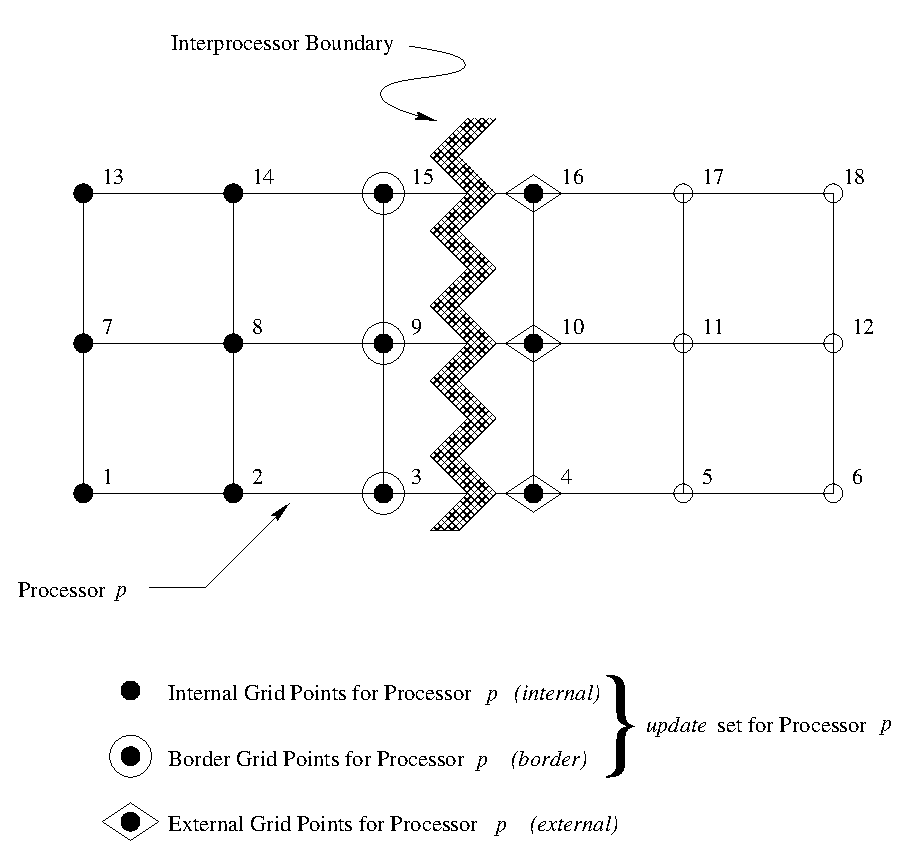
\epsfig{file=./figs/aztec_decomp.eps,height=4.5in,clip}}
      \vspace{0.5em}
    \end{minipage}}
  \caption{Example partitioning of a finite element grid.} \label{aztec_decomp}
\end{figure}
Since these sets of indices are used exclusively to reference specific vector
components, the same names (i.e., {\it update\/}, {\it internal\/}, {\it
  border\/} and {\it external\/}) are sometimes used below to describe the
vector elements themselves.  Having generalized these labels, the three types
of vector elements are distinguished by locally storing the {\it internal}
components first, followed by the {\it border} components and finally by the
{\it external} components.  In addition, all {\it external} components received
from the same processor are stored consecutively.  Below we summarize the
nomenclature for a processor with $N$ total elements where {\it N\_internal\/},
{\it N\_border\/}, and {\it N\_external\/} elements are distributed over the
sets {\it internal\/}, {\it border\/} and {\it external\/} respectively.
\vskip .2in
\begin{center}
  \begin{tabularx}{\textwidth}{|l|X|X|} \hline
    \bf set & \bf description & \bf local numbering \\ \hline \hline
    \it internal & updated w/o communication & $0$ to $ N\_internal - 1$.\\
    \hline
    \it border & updated with communication & $N\_internal$ to $N\_internal
    + N\_border - 1$. \\ \hline
    \it external & not updated but used to update \it border. & $N\_internal +
    N\_border$ to $N - 1$. Elements received from the same processor are
    numbered consecutively. \\ \hline
  \end{tabularx}
\end{center}
\vskip .2in

Similar to vectors, a subset of matrix non-zeros is stored on each processor.
In particular, each processor stores only those rows which correspond to its
{\it update\/} set.  For example, if vector element $i$ is updated on processor
$p$, then processor $p$ also stores all the non-zeros of row $i$ in the matrix.
Further, the local numbering of vector elements on a specific processor induces
a local numbering of matrix rows and columns.  For example, if vector element
$k$ is locally numbered as $k_l$, then all references to row $k$ or column $k$
in the matrix would be locally numbered as $k_l$.  Thus, each processor
contains a submatrix whose row and column entries correspond to variables
defined on this processor.

The remainder of this section describes the two sparse matrix formats that are
used to store the local renumbered submatrix. These two sparse matrix formats
correspond to common formats used in serial computations.

\subsection{Distributed Modified Sparse Row (DMSR) Format} \label{DMSR Format}

The DMSR format is a generalization of the MSR format~\cite{concurrency}. The
data structure consists of an integer vector {\it bindx\/} and a double
precision vector {\it val\/} each of length {\it N\_nonzeros + 1} where {\it
  N\_nonzeros} is the number of nonzeros in the local submatrix.  For a
submatrix with $m$ rows the DMSR arrays are as follows:
%
\vspace{2em}
%{\flushleft{\bf Descriptions} \hrulefill}
%\nopagebreak% \\[0.5em]
\begin{tabbing}
$\hphantom{rp}$
\= {\it bindx {\bf :}\/} \\[0.3em]
\>$\hphantom{rpntrsqv}$
  \= {\it bindx[0]\/} \hskip 0.9in \= = \= m + 1 \\
\>\> {\it bindx[k+1] - bindx[k]\/} \> = \> number of nonzero
                                           off-diagonal elements
                                           in {\it k\/}'th \\
\>\>                               \>   \> row, $k < m $ \\
\>\> {\it bindx[$k_s ... k_e$]\/}  \> = \> column indices of the
                                           off-diagonal
                                           nonzeros in row\\
\>\>                               \>   \> $k$ where
                                           $k_s$ = {\it bindx[k]} and
                                           $k_e$ = {\it bindx[k+1]-1}.\\[0.8em]
\> {\it val {\bf :}\/} \\[0.3em]
\>\> {\it val[k] \/}               \> = \> $ A_{kk}, k < m $ \\
\>\> {\it val[$k_i$] \/}   \> = \> the ($k$, {\it bindx[$k_i$] \/})'th
                                           matrix element where \\
\>\>                               \>   \> $k_s \leq k_i \leq k_e $
                                           with $k_s$ and $k_e$ as defined
                                           above.
\end{tabbing}
%
\vspace{1em}
Note: {\it val[m]\/} is not used. See~\cite{sparker2} for a detailed
discussion of the MSR format.

\subsection{Distributed Variable Block Row (DVBR) Format} \label{DVBR Format}

The Distributed Variable Block Row (DVBR) format is a generalization of the VBR
format~\cite{sparker2}.  The data structure consists of a double precision
vector {\it val\/} and five integer vectors: {\it indx\/}, {\it bindx\/}, {\it
  rpntr\/}, {\it cpntr\/} and {\it bpntr\/}.  The format is best suited for
sparse block matrices of the form
\[
A = \left( \begin{array}{cccc}
        A_{00} & A_{01} & \cdots & A_{0k} \\
        A_{10} & A_{11} & \cdots & A_{1k} \\
        \vdots & & \ddots & \vdots \\
        A_{m0} & \cdots & \cdots & A_{mk} \end{array}
\right)
\]
where $A_{ij}$ denotes a block (or submatrix). In a sparse block matrix, some
of these blocks would be entirely zero while others may be dense. The DVBR
vectors are described below for a matrix with $M \times K$ blocks.
%
\vspace{1em}
%{\flushleft{\bf Descriptions} \hrulefill}
%\nopagebreak %\\[0.5em]
\begin{tabbing}
$\hphantom{rp}$
\= {\it rpntr[0 ... M] {\bf :}\/} \\[0.3em]
\>$\hphantom{rpntrsqv}$
  \= {\it rpntr[0]\/} \hskip 0.9in \= = \= 0 \\
\>\> {\it rpntr[k+1] - rpntr[k]\/} \> = \> number of rows in {\it
                                           k\/}'th block row \\[0.8em]
\> {\it cpntr[0 ... K] {\bf :}\/} \\[0.3em]
\>\> {\it cpntr[0]\/}              \> = \> 0 \\
\>\> {\it cpntr[k+1] - cpntr[k]\/} \> = \> number of columns in {\it
                                           k\/}'th block column \\[0.8em]
\> {\it bpntr[0 ... M] {\bf :}\/} \\[0.3em]
\>\> {\it bpntr[0]\/}              \> = \> 0 \\
\>\> {\it bpntr[k+1] - bpntr[k]\/} \> = \> number of nonzero blocks in the
                                           {\it k\/}'th block row\\[0.8em]
\> {\it bindx[0 ... bpntr[M] - 1] {\bf :}\/}\\[0.3em]
\>\> {\it bindx[$k_s ... k_e$]\/}  \> = \> block column indices of nonzero
                                           blocks in block row $k$ \\
\>\>                               \>   \> where $k_s$ = {\it bpntr[k]} and
                                           $k_e$ = {\it bpntr[k+1]}-1 \\[0.8em]
\> {\it indx[0 ... bpntr[M] ] {\bf :}\/}\\[0.3em]
\>\> {\it indx[0]\/}               \> = \> 0 \\
\>\> {\it indx[$k_i$+1] - indx[$k_i$]\/}\> = \> number of nonzeros in
                                                the ($k$, {\it
                                                bindx[$k_i$]\/})'th
                                                block \\
\>\>                               \>   \> where $k_s \leq k_i \leq
                                           k_e$ with $k_s$ and $k_e$
                                           as defined \\
\>\>                               \>   \> above. \\[0.8em]
\> {\it val[0 ... indx[bpntr[M]] - 1 ] {\bf :}\/}\\[0.3em]
\>\> {\it val[$i_s ... i_e$]\/}  \> = \> nonzeros in the ($k$, {\it
     bindx[$k_i$]\/})'th block stored in \\
\>\>                             \>   \> column major order where
                                         $k_i$ is as defined above, \\
\>\>                             \>   \> $i_s$ = {\it indx[$k_i$]} and
                                         $i_e$ = {\it indx[$k_i$+1]}-1
\end{tabbing}
\vspace{1em}
%
See~\cite{sparker2} for a detailed discussion of the VBR format.

%%% Local Variables:
%%% mode: latex
%%% TeX-master: "az_ug_20"
%%% End:


\section{High Level Data Interface\label{highlevel_data_inter}}

Setting up the distributed format described in Section~\ref{data_formats} for
the local submatrix on each processor can be quite cumbersome. In particular,
the user must determine a mapping between the global numbering scheme and a
local scheme which facilitates proper communication.  Further, a number of
additional variables must be set for communication and synchronization (see
Section~\ref{advanced_topics}).  In this section we describe a simpler data
format that is used in conjunction with a transformation function to generate
data structures suitable for \Az{}.  The new format allows the user to specify
the rows in a natural order as well as to use global column numbers in the {\it
  bindx} array.  To use the transformation function the user supplies the {\it
  update\/} set and the submatrix for each processor.  Unlike the previous
section, however, the submatrix is specified using the global coordinate
numbering instead of the local numbering required by \Az{}. This procedure
greatly facilitates matrix specification and is the main advantage of the
transformation software.

On a given processor, the {\it update\/} set (i.e.  vector element assignment
to processors) is defined by initializing the array {\it update\/} on each
processor so that it contains the global index of each element assigned to the
processor. The {\it update} array must be sorted in ascending order (i.e. $ i <
j \Rightarrow update[i] < update[j]$). This sorting can be performed using the
\Az{} function {\sf AZ\_sort}. Matrix specification occurs using the arrays
defined in the previous section. However, now the local rows are defined in the
same order as the {\it update} array and column indices (e.g. {\it bindx}) are
given as global column indices.  To illustrate this in more detail, consider
the following example matrix:
\[
A = \pmatrix{ a_{00} & a_{01} &        & a_{03} & a_{04} &        \cr
              a_{10} & a_{11} &        & a_{13} &        &        \cr
                     &        & a_{22} & a_{23} & a_{24} & a_{25} \cr
              a_{30} & a_{31} & a_{32} & a_{33} & a_{34} & a_{35} \cr
              a_{40} &        & a_{42} & a_{43} & a_{44} &        \cr
                     &        & a_{52} & a_{53} &        & a_{55} } .
\]
Figure~\ref{init_input} illustrates the information corresponding to a
particular matrix partitioning that is specified by the user as input to the
data transformation tool.
\begin{figure}[Htbp]
  \shadowbox{
%    \begin{minipage}{\textwidth}
    \begin{minipage}{6.2in}
      \vspace{0.5em}
      {\large \flushleft{\bf Example}} \hrulefill %
      \vspace{0.5em}
%%%
\begin{tabbing}
\tt
\hsp proc 0: \\
\>  \hsp N\_update: \in  3 \\
\>  \>   update:    \>   0 \sp 1  \sp 3 \\
\>  \>   bindx:     \>   4       \>   7       \>   9       \sp 14     \sp 1
                    \sp  3       \sp  4       \sp  0       \sp  3     \sp  0
                    \sp  1       \sh  2       \sh  4       \sh  5\\
\>  \>   val:       \>  $a_{00}$ \>  $a_{11}$ \>  $a_{33}$ \> \hskip .05in -  \> $a_{01}$
                    \>  $a_{03}$ \>  $a_{04}$ \>  $a_{10}$ \> $a_{13}$\>$a_{30}$
                    \>  $a_{31}$ \bb $a_{32}$ \bb $a_{34}$ \bb $a_{35}$\\
\>-----------------------------------------------------------------------------------------------------------\\
\>  proc 1:\\
\>  \>   N\_update: \>   1\\
\>  \>   update:    \>   4\\
\>  \>   bindx:     \>   2 \>   5  \>   0 \>   3  \>  2 \\
\>  \>   val:       \>$a_{44}$\>\hskip .025in -\>$a_{40}$\>$a_{43}$\>$a_{42}$\\
\>-----------------------------------------------------------------------------------------------------------\\
\>  proc 2:\\
\>  \>   N\_update: \>   2\\
\>  \>   update:    \>   2 \>   5\\
\>  \>   bindx:     \>   3 \>   6  \>   8 \>   3  \>  4  \> 5  \> 2  \> 3\\
\>  \>   val:       \>$a_{22}$\>$a_{55}$\>\hskip .025in -\>$a_{23}$\>
                        $a_{24}$\>$a_{25}$\>$a_{52}$\>$a_{53}$
\end{tabbing}
%%%
      \vspace{0.5em}
    \end{minipage}}
  \caption{User input (MSR format) to initialize the sample matrix problem.}
  \label{init_input}
\end{figure}
%It should also be note that though this example
%considers only the sparsity pattern of the matrix, it is possible to
%specify the actual nonzero entries as well at the start of the calculation.
Using this information, {\sf AZ\_transform}
\begin{itemize}
\item determines the sets {\it internal}, {\it border} and
      {\it external}.
\item determines the local numbering:
      {\it update\_index[i]} is the local numbering for
      {\it update[i]} while {\it extern\_index[i]} is the local
      numbering for {\it external[i]}.
\item permutes and renumbers the local submatrix rows and columns so that
      they now correspond to the new ordering.
\item computes additional information
      (e.g. the number of internal, border and external components on this
      processor) and
      stores this in {\it data\_org\/} (see Section~\ref{advanced_topics}).
\end{itemize}
A sample transformation is given in Figure~\ref{init_mv_structs}
%
\begin{figure}[Htbp]
  \shadowbox{
%    \begin{minipage}{\textwidth}
    \begin{minipage}{6.2in}
      \vspace{0.5em}
      {\large \flushleft{\bf Example}} \hrulefill %
      \vspace{0.5em}
%%%
\begin{verbatim}
init_matrix_vector_structures(bindx, val, update, external,
                              update_index, extern_index, data_org);
{
  AZ_read_update(update, N_update);
  create_matrix(bindx, val, update, N_update);
  AZ_transform(bindx, val, update, external, update_index,
               extern_index, data_org, N_update);
}
\end{verbatim}
%%%
      \vspace{0.1em}
    \end{minipage}}
  \caption{{\sf init\_matrix\_vector\_structures}.}\label{init_mv_structs}
\end{figure}
%
and is found in the file \verb'az\_app\_utils.c'.  {\sf AZ\_read\_update} is an
\Az{} utility which reads a file and assigns elements to {\it update\/}.  The
user supplied routine {\sf create\_matrix} creates an MSR or VBR matrix using
the global numbering.  Once transformed the matrix can now be used within
\Az{}.

%%% Local Variables:
%%% mode: latex
%%% TeX-master: "az_ug_20"
%%% End:


%
% This section includes brief examples, including all source
% code and gnuplot images where possible, of a geometric problem,
% a graph problem, and a hypergraph problem.  
%
\chapter{Examples}
\label{cha:ex}

This chapter begins with a very simple example.  We use the Zoltan
library in a parallel application to partition a small set of 
objects, each of which has only a global ID and a weight.

We follow this with three more realistic examples.
These examples use the Zoltan library to apply a geometric method,
a graph method and a then hypergraph method to a small mesh, graph
and hypergraph respectively.

If you have the Zoltan source code, you can find these
examples in the \textbf{examples/C} directory.  The versions
found in the source code include code to
display the initial partitioning followed by Zoltan's computed
partitioning.  It may be helpful to compile and run them, and
then try changing parameters 
to see how the partitioning is affected.  Consult the Zoltan
User's Guide at
\url{http://www.cs.sandia.gov/Zoltan/ug_html/ug.html}
for a complete list of all partitioning methods and all of the
parameters for each partitioning method.

The next four examples are written in C.  At the end of this section,
we also provide a C++ version of the geometric example.

As you read through these examples you will see that, regardless 
of the load balancing method chosen, every program must:

\begin{itemize}
\item initialize the Zoltan library
\item supply load balancing parameters to Zoltan
\item define query functions that Zoltan will use to obtain information from the application about the objects to be partitioned
\item call Zoltan\_LB\_Partition to begin the load balancing calculation
\item free memory allocated by Zoltan when done
\end{itemize}

\clearpage
\section{A very simple partitioning method}

This example is a C program which uses Zoltan to partition
in parallel 36 objects, each of which has a weight.  The goal is
to balance the weights across the parallel application.

It uses the Zoltan method called BLOCK, which simply assignes 
the first $n/p$ data objects to the first process and so on.
This method really exists as an example for developers
to learn how to write partitioning methods.  
It can also be used for testing in applications, but was never
intended to be a serious partitioning strategy for real applications.
However, it is a good choice for our first example.  

If you are a new user of Zoltan, you may want to initially get your
application working with the BLOCK method.  Once you have
that first step accomplished, you can modify it to use one of the
other partitioning methods.

In order to use the BLOCK method, we must define two query functions:

\begin{itemize}
\item A function of type ZOLTAN\_NUM\_OBJ\_FN which provides the number of objects belonging to this process.  In our example we call this function \textbf{get\_number\_of\_objects}.
\item A function of type ZOLTAN\_OBJ\_LIST\_FN which supplies the global IDs and optional weights for the objects belonging to the process.  We name this function \textbf{get\_object\_list}.
\end{itemize}

The \textbf{ZOLTAN\_*} function prototyes named above
are defined in the Zoltan file \textbf{include/zoltan.h}.

Zoltan requires that the parallel application supply a unique 
global ID to identify each of the objects to be partitioned.
Zoltan is very flexible about the data type used to represent
a global ID, and only requires that it be allowed to represent
your global ID internally as an array of integers of some user-defined
length.  Zoltan also permits the use of an additional set of
IDs that are local to a process.  If you supply these optional local IDs,
Zoltan will also include them when querying your application for data.

A version of the 
code listed below may be found in the Zoltan source in file
\textbf{examples/C/simpleBLOCK.c}. 

\begin{flushleft}
\begin{verbatim}
#include <mpi.h>
#include <stdio.h>
#include <stdlib.h>
#include "zoltan.h"

static int numObjects = 36;
static int numProcs, myRank, myNumObj;
static int myGlobalIDs[36];

static float objWeight(int globalID)
{
float w;     /* simulate an initial imbalance */
  if (globalID % numProcs == 0) w = 3;
  else                          w = (globalID % 3 + 1);
  return w;
}
static int get_number_of_objects(void *data, int *ierr)
{
  *ierr = ZOLTAN_OK;
  return myNumObj;
}
static void get_object_list(void *data, int sizeGID, int sizeLID,
            ZOLTAN_ID_PTR globalID, ZOLTAN_ID_PTR localID,
            int wgt_dim, float *obj_wgts, int *ierr)
{
int i;
  *ierr = ZOLTAN_OK;
  for (i=0; i<myNumObj; i++){
    globalID[i] = myGlobalIDs[i];
    if (obj_wgts) obj_wgts[i] = objWeight(myGlobalIDs[i]);
  }
}
int main(int argc, char *argv[])
{
  int rc, i, changes, numGidEntries, numLidEntries, numImport, numExport;
  float ver;
  struct Zoltan_Struct *zz;
  ZOLTAN_ID_PTR importGlobalGids, importLocalGids;
  ZOLTAN_ID_PTR exportGlobalGids, exportLocalGids; 
  int *importProcs, *importToPart, *exportProcs, *exportToPart;

  /******************************************************************
  ** Initialize MPI and Zoltan
  ******************************************************************/

  MPI_Init(&argc, &argv);
  MPI_Comm_rank(MPI_COMM_WORLD, &myRank);
  MPI_Comm_size(MPI_COMM_WORLD, &numProcs);

  rc = Zoltan_Initialize(argc, argv, &ver);

  if (rc != ZOLTAN_OK){
    printf("Error initializing Zoltan\n");
    MPI_Finalize();
    exit(0);
  }

  /******************************************************************
  ** Create a simple initial partitioning for this example
  ******************************************************************/

  for (i=0, myNumObj=0; i<numObjects; i++)
    if (i % numProcs == myRank)
      myGlobalIDs[myNumObj++] = i+1;

  /******************************************************************
  ** Create a Zoltan library structure for this instance of load
  ** balancing.  Set the parameters and query functions.
  ******************************************************************/

  zz = Zoltan_Create(MPI_COMM_WORLD);

  /* General parameters */

  Zoltan_Set_Param(zz, "LB_METHOD", "BLOCK");  /* name of Zoltan method */
  Zoltan_Set_Param(zz, "NUM_GID_ENTRIES", "1"); /* size of global ID    */
  Zoltan_Set_Param(zz, "NUM_LID_ENTRIES", "0"); /* no local IDs         */
  Zoltan_Set_Param(zz, "OBJ_WEIGHT_DIM", "1"); /* weights are 1 float   */

  /* Query functions */

  Zoltan_Set_Num_Obj_Fn(zz, get_number_of_objects, NULL);
  Zoltan_Set_Obj_List_Fn(zz, get_object_list, NULL);

  /******************************************************************
  ** Call Zoltan to partition the objects.
  ******************************************************************/

  rc = Zoltan_LB_Partition(zz, /* input (all remaining fields are output) */
        &changes,        /* 1 if partitioning was changed, 0 otherwise */ 
        &numGidEntries,  /* Number of integers used for a global ID */
        &numLidEntries,  /* Number of integers used for a local ID */
        &numImport,      /* Number of objects to be sent to me */
        &importGlobalGids,  /* Global IDs of objects to be sent to me */
        &importLocalGids,   /* Local IDs of objects to be sent to me */
        &importProcs,    /* Process rank for source of each incoming object */
        &importToPart,   /* New partition for each incoming object */
        &numExport,      /* Number of objects I must send to other processes*/
        &exportGlobalGids,  /* Global IDs of the objects I must send */
        &exportLocalGids,   /* Local IDs of the objects I must send */
        &exportProcs,    /* Process to which I send each of the objects */
        &exportToPart);  /* Partition to which each object will belong */

  if (rc != ZOLTAN_OK){
    printf("Error in Zoltan library\n");
    MPI_Finalize();
    Zoltan_Destroy(&zz);
    exit(0);
  }

  /******************************************************************
  ** Here you would send the objects to their new partitions.
  ******************************************************************/

  /******************************************************************
  ** Free the arrays allocated by Zoltan_LB_Partition, and free
  ** the storage allocated for the Zoltan structure.
  ******************************************************************/

  Zoltan_LB_Free_Part(&importGlobalGids, &importLocalGids, 
                      &importProcs, &importToPart);
  Zoltan_LB_Free_Part(&exportGlobalGids, &exportLocalGids, 
                      &exportProcs, &exportToPart);

  Zoltan_Destroy(&zz);

  MPI_Finalize();

  return 0;
}
\end{verbatim}
\end{flushleft}

\clearpage
\section{Geometric, Graph and Hypergraph Examples}

The simple graph used in all three examples in this section
is illustrated in Figure~\ref{fig:mesh25}.
It is defined in the Zoltan source file \textbf{examples/C/simpleGraph.h},
which is listed in Figure~\ref{fig:simpleGraphDotH}.

\begin{figure}[bottom]
\label{fig:mesh25}
\begin{center}
\begin{verbatim}
   21----22----23----24---25
   |     |     |     |    |
   16----17----18----19---20
   |     |     |     |    |
   11----12----13----14---15
   |     |     |     |    |
   6-----7-----8-----9----10
   |     |     |     |    |
   1-----2-----3-----4----5
\end{verbatim}
\caption{Mesh with 25 vertices}
\end{center}
\end{figure}

\begin{figure}
\label{fig:simpleGraphDotH}
\begin{flushleft}
\begin{verbatim}
#ifndef SIMPLEGRAPH_H
#define SIMPLEGRAPH_H
static int numvertices=25;
static int simpleNumEdges[25] = {
2, 3, 3, 3, 2,
3, 4, 4, 4, 3,
3, 4, 4, 4, 3,
3, 4, 4, 4, 3,
2, 3, 3, 3, 2
};
static int edges[25][4]={
{2,6},       /* adjacent to vertex 1 */
{1,3,7},     /* adjacent to vertex 2 */
{2,8,4},
{3,9,5},
{4,10},
{1,7,11},
{6,2,8,12},
{7,3,9,13},
{8,4,10,14},
{9,5,15},
{6,12,16},
{11,7,13,17},
{12,8,14,18},
{13,9,15,19},
{14,10,20},
{11,17,21},
{16,12,18,22},
{17,13,19,23},
{18,14,20,24},
{19,15,25},
{16,22},
{21,17,23},
{22,18,24},
{23,19,25},
{24,20}      /* adjacent to vertex 25 */
};
#endif
\end{verbatim}
\end{flushleft}
\caption{Adjacencies for a simple mesh}
\end{figure}


\clearpage
\subsection{Recursive Coordinate Bisection}
\label{sec:rcb}

This example uses \emph{Recursive Coordinate Bisection}, 
one of Zoltan's geometric methods, to partition
the vertices of the simple mesh.  This method will use
the coordinates of each vertex, and the weight of each
vertex, in determining a partitioning.  The mesh adjacencies are
irrelevant in this example, although we define the weight of
a vertex to be the number of mesh neighbors it has.

First we will define the query functions required by RCB.
The full source code for this example may be found in
\textbf{examples/C/simpleRCB.c}.

\subsubsection{Application defined query functions}

We must define four query functions.  The function prototyes named 
below are defined in the Zoltan file \textbf{include/zoltan.h}.

\begin{itemize}
\item A function of type ZOLTAN\_NUM\_OBJ\_FN (Figure~\ref{fig:NumObj}) which provides the number of objects belonging to this process 
\item A function of type ZOLTAN\_OBJ\_LIST\_FN (Figure~\ref{fig:ObjList}) which supplies the global IDs and optional weights for the objects belonging to the process
\item A function of type ZOLTAN\_NUM\_GEOM\_FN (Figure~\ref{fig:NumGeom}) which provides the dimension of the objects
\item A function of type ZOLTAN\_GEOM\_MULTI\_FN (Figure~\ref{fig:GeomMulti}) which supplies the coordinates of the objects and optionally their weights
\end{itemize}

An alternative to defining a single ZOLTAN\_OBJ\_LIST\_FN is to define
a ZOLTAN\_FIRST\_OBJ\_FN and a ZOLTAN\_NEXT\_OBJ\_FN.  The first function
would return the global ID for first object.  Each call to the second function would
return a subsequent global ID.

An alternative to ZOLTAN\_GEOM\_MULTI\_FN is to define a ZOLTAN\_GEOM\_FN which
returns the coordinates for a single object rather than for a list
of objects.

The variables referred to in the query functions below were defined in the header
file ~\ref{fig:simpleGraphDotH} to describe the mesh in Figure ~\ref{fig:mesh25}.


\begin{figure}
\begin{flushleft}
\begin{verbatim}
static int get_number_of_objects(void *data, int *ierr)
{
int i, numobj=0;

  for (i=0; i<simpleNumVertices; i++){
    if (i % numProcs == myRank) numobj++;
  }
  *ierr = ZOLTAN_OK;
  return numobj;
}
\end{verbatim}
\end{flushleft}
\caption{A ZOLTAN\_NUM\_OBJ\_FN query function}
\label{fig:NumObj}
\end{figure}

\begin{figure}
\begin{flushleft}
\begin{verbatim}
static void get_object_list(void *data, int sizeGID, int sizeLID,
            ZOLTAN_ID_PTR globalID, ZOLTAN_ID_PTR localID,
                  int wgt_dim, float *obj_wgts, int *ierr)
{
int i, next;

  if ( (sizeGID != 1) || (sizeLID != 1) || (wgt_dim != 1)){ 
    *ierr = ZOLTAN_FATAL;
    return;
  }

  for (i=0, next=0; i<simpleNumVertices; i++){
    if (i % numProcs == myRank){
      globalID[next] = i+1;   /* application wide global ID */
      localID[next] = next;   /* process specific local ID  */
      obj_wgts[next] = (float)simpleNumEdges[i];  /* weight */
      next++;
    }
  }

  *ierr = ZOLTAN_OK;

  return;
}
\end{verbatim}
\end{flushleft}
\caption{A ZOLTAN\_OBJ\_LIST\_FN query function}
\label{fig:ObjList}
\end{figure}

\begin{figure}
\begin{flushleft}
\begin{verbatim}
static int get_num_geometry(void *data, int *ierr)
{
  *ierr = ZOLTAN_OK;
  return 2;
}
\end{verbatim}
\end{flushleft}
\caption{A ZOLTAN\_NUM\_GEOM\_FN query function}
\label{fig:NumGeom}
\end{figure}

\begin{figure}
\begin{flushleft}
\begin{verbatim}
static void get_geometry_list(void *data, int sizeGID, int sizeLID,
                      int num_obj,
             ZOLTAN_ID_PTR globalID, ZOLTAN_ID_PTR localID,
             int num_dim, double *geom_vec, int *ierr)
{
int i;
int row, col;
   
  if ( (sizeGID != 1) || (sizeLID != 1) || (num_dim != 2)){
    *ierr = ZOLTAN_FATAL; 
    return;
  }
    
  for (i=0;  i < num_obj ; i++){
    row = (globalID[i] - 1) / 5;
    col = (globalID[i] - 1) % 5;
  
    geom_vec[2*i] = (double)col;
    geom_vec[2*i + 1] = (double)row;
  }

  *ierr = ZOLTAN_OK;
  return;
} 
\end{verbatim}
\end{flushleft}
\caption{A ZOLTAN\_GEOM\_MULTI\_FN query function}
\label{fig:GeomMulti}
\end{figure}

\clearpage
\subsubsection{Calling the Zoltan library}

The source code below may be found in the file
\textbf{examples/C/simpleRCB.c}.
More information about RCB parameters
may be found in the Zoltan User's Guide at
\url{http://www.cs.sandia.gov/Zoltan/ug_html/ug_alg_rcb.html}.

\begin{flushleft}
\begin{verbatim}
#include <mpi.h>
#include <stdio.h>
#include <stdlib.h>
#include "zoltan.h"
#include "simpleGraph.h"
#include "simpleQueries.h"

int main(int argc, char *argv[])
{
  int rc, i, ngids, nextIdx;
  struct Zoltan_Struct *zz;
  int changes, numGidEntries, numLidEntries, numImport, numExport;
  ZOLTAN_ID_PTR importGlobalGids, importLocalGids;
  ZOLTAN_ID_PTR exportGlobalGids, exportLocalGids; 
  int *importProcs, *importToPart, *exportProcs, *exportToPart;
  float *wgt_list, ver;
  int *gid_flags, *gid_list, *lid_list;

  /******************************************************************
  ** Initialize MPI and Zoltan
  ******************************************************************/

  MPI_Init(&argc, &argv);
  MPI_Comm_rank(MPI_COMM_WORLD, &myRank);
  MPI_Comm_size(MPI_COMM_WORLD, &numProcs);

  rc = Zoltan_Initialize(argc, argv, &ver);

  if (rc != ZOLTAN_OK){
    MPI_Finalize();
    exit(0);
  }
\end{verbatim}
\end{flushleft}

\clearpage
\begin{flushleft}
\begin{verbatim}
  /******************************************************************
  ** Create a Zoltan library structure for this instance of load
  ** balancing.  Set the parameters and query functions that will
  ** govern the library's calculation.  See the Zoltan User's
  ** Guide for the definition of these and many other parameters.
  ******************************************************************/

  zz = Zoltan_Create(MPI_COMM_WORLD);

  /* General parameters */

  Zoltan_Set_Param(zz, "DEBUG_LEVEL", "0");
  Zoltan_Set_Param(zz, "LB_METHOD", "RCB");
  Zoltan_Set_Param(zz, "NUM_GID_ENTRIES", "1"); 
  Zoltan_Set_Param(zz, "NUM_LID_ENTRIES", "1");
  Zoltan_Set_Param(zz, "OBJ_WEIGHT_DIM", "1");
  Zoltan_Set_Param(zz, "RETURN_LISTS", "ALL");

  /* RCB parameters */

  Zoltan_Set_Param(zz, "KEEP_CUTS", "1"); 
  Zoltan_Set_Param(zz, "RCB_OUTPUT_LEVEL", "0");
  Zoltan_Set_Param(zz, "RCB_RECTILINEAR_BLOCKS", "1"); 

  /* Query functions - defined in simpleQueries.h, to return
   * information about objects defined in simpleGraph.h      */

  Zoltan_Set_Num_Obj_Fn(zz, get_number_of_objects, NULL);
  Zoltan_Set_Obj_List_Fn(zz, get_object_list, NULL);
  Zoltan_Set_Num_Geom_Fn(zz, get_num_geometry, NULL);
  Zoltan_Set_Geom_Multi_Fn(zz, get_geometry_list, NULL);

\end{verbatim}
\end{flushleft}

\clearpage
\begin{flushleft}
\begin{verbatim}

  /******************************************************************
  ** Zoltan can now partition the vertices in the simple mesh.
  ** In this simple example, we assume the number of partitions is
  ** equal to the number of processes.  Process rank 0 will own
  ** partition 0, process rank 1 will own partition 1, and so on.
  ******************************************************************/

  rc = Zoltan_LB_Partition(zz, /* input (all remaining fields are output) */
        &changes,        /* 1 if partitioning was changed, 0 otherwise */ 
        &numGidEntries,  /* Number of integers used for a global ID */
        &numLidEntries,  /* Number of integers used for a local ID */
        &numImport,      /* Number of vertices to be sent to me */
        &importGlobalGids,  /* Global IDs of vertices to be sent to me */
        &importLocalGids,   /* Local IDs of vertices to be sent to me */
        &importProcs,    /* Process rank for source of each incoming vertex */
        &importToPart,   /* New partition for each incoming vertex */
        &numExport,      /* Number of vertices I must send to other processes*/
        &exportGlobalGids,  /* Global IDs of the vertices I must send */
        &exportLocalGids,   /* Local IDs of the vertices I must send */
        &exportProcs,    /* Process to which I send each of the vertices */
        &exportToPart);  /* Partition to which each vertex will belong */

  if (rc != ZOLTAN_OK){
    printf("sorry...\n");
    MPI_Finalize();
    Zoltan_Destroy(&zz);
    exit(0);
  }

  /******************************************************************
  ** In a real application, you would rebalance the problem now by
  ** sending the objects to their new partitions.
  ******************************************************************/

\end{verbatim}
\end{flushleft}

\clearpage
\begin{flushleft}
\begin{verbatim}

  /******************************************************************
  ** Free the arrays allocated by Zoltan_LB_Partition, and free
  ** the storage allocated for the Zoltan structure.
  ******************************************************************/

  Zoltan_LB_Free_Part(&importGlobalGids, &importLocalGids, 
                      &importProcs, &importToPart);
  Zoltan_LB_Free_Part(&exportGlobalGids, &exportLocalGids, 
                      &exportProcs, &exportToPart);

  Zoltan_Destroy(&zz);

  /**********************
  ** all done ***********
  **********************/

  MPI_Finalize();

  return 0;
}

\end{verbatim}
\end{flushleft}

\clearpage
\subsection{A graph problem}

In this section we provide an example of a parallel C program
that uses the Zoltan library to partition the simple graph that
was pictured in Figure~\ref{fig:mesh25}.  You can compile
and run this example if you have the Zoltan source code.  It is
in the examples directory, in file \textbf{examples/C/simpleGRAPH.c}.

\subsubsection{Application defined query functions}

We must define four query functions in order to use the
particular graph submethod we chose for this example.  See the
User's Guide at
\url{http://www.cs.sandia.gov/Zoltan/ug_html/ug_alg_parmetis.html} for
the requirements of other submethods.

The function prototypes referred to below
are defined in the Zoltan file \textbf{include/zoltan.h}.
The four query functions are:

\begin{itemize}
\item A function of type ZOLTAN\_NUM\_OBJ\_FN (Figure~\ref{fig:NumObj}) which provides the number of objects belonging to this process 
\item A function of type ZOLTAN\_OBJ\_LIST\_FN (Figure~\ref{fig:ObjList}) which supplies the global IDs and optional weights for the objects belonging to the process
\item A function of type ZOLTAN\_NUM\_EDGES\_MULTI\_FN (Figure~\ref{fig:NumEdges}) which provides the number of edges for each object
\item A function of type ZOLTAN\_EDGE\_LIST\_MULTI\_FN (Figure~\ref{fig:EdgeListMulti})
which, for a given object ID, responds with the IDs for
each adjacent object, the process owning that adjacent object, and optionally a weight
for each edge
\end{itemize}

An alternative to defining a single ZOLTAN\_OBJ\_LIST\_FN is to define
a ZOLTAN\_FIRST\_OBJ\_FN and a ZOLTAN\_NEXT\_OBJ\_FN.  The first function
would return the global ID for first object.  Each call to the second function would
return a subsequent global ID.

An alternative to defining a ZOLTAN\_NUM\_EDGES\_MULTI\_FN is to 
define a ZOLTAN\_NUM\_EDGES\_FN, which returns the number of adjacent
objects for a single object ID.

An alternative to defining a ZOLTAN\_EDGE\_LIST\_MULTI\_FN is to 
define a ZOLTAN\_EDGE\_LIST\_FN, which
returns the same information but for a single object.

The variables used in these query functions to describe our simple graph
refer to those defined in \textbf{examples/C/simpleGraph.h} which were shown in
Figure~\ref{fig:simpleGraphDotH}.

\begin{figure}
\begin{flushleft}
\begin{verbatim}
static void get_num_edges_list(void *data, int sizeGID, int sizeLID,
        int num_obj, ZOLTAN_ID_PTR globalID, ZOLTAN_ID_PTR localID,
        int *numEdges, int *ierr)
{
int i, idx;

  if ( (sizeGID != 1) || (sizeLID != 1)){
    *ierr = ZOLTAN_FATAL;
    return;
  }

  for (i=0;  i < num_obj ; i++){
    idx = globalID[i] - 1;
    numEdges[i] = simpleNumEdges[idx];
  }

  *ierr = ZOLTAN_OK;
  return;
}
\end{verbatim}
\end{flushleft}
\caption{A ZOLTAN\_NUM\_EDGES\_MULTI\_FN query function}
\label{fig:NumEdges}
\end{figure}

\begin{figure}
\begin{flushleft}
\begin{verbatim}
static void get_edge_list(void *data, int sizeGID, int sizeLID,
        int num_obj, ZOLTAN_ID_PTR globalID, ZOLTAN_ID_PTR localID,
        int *num_edges, ZOLTAN_ID_PTR nborGID, int *nborProc,
        int wgt_dim, float *ewgts, int *ierr)
{
int i, j, idx;
ZOLTAN_ID_PTR nextID;
int *nextProc;

  if ( (sizeGID != 1) || (sizeLID != 1) || (wgt_dim != 0)){
    *ierr = ZOLTAN_FATAL;
    return;
  }

  nextID = nborGID;
  nextProc = nborProc;

  for (i=0;  i < num_obj ; i++){
    idx = globalID[i] - 1;
    if (num_edges[i] != simpleNumEdges[idx]){
      *ierr = ZOLTAN_FATAL;
      return;
    }
    for (j=0; j<num_edges[i]; j++){
      *nextID++ = simpleEdges[idx][j];
      *nextProc++ = (simpleEdges[idx][j] - 1) % numProcs;
    }
  }

  *ierr = ZOLTAN_OK;

  return;
}
\end{verbatim}
\end{flushleft}
\caption{A ZOLTAN\_EDGE\_LIST\_MULTI\_FN query function}
\label{fig:EdgeListMulti}
\end{figure}

\clearpage

\subsubsection{Calling the Zoltan library}

This code may be found in the 
file \textbf{examples/C/simpleGRAPH.c}.
More information about graph parameters 
may be found in the Zoltan User's Guide at
\url{http://www.cs.sandia.gov/Zoltan/ug_html/ug_alg_parmetis.html}.

\begin{flushleft}
\begin{verbatim}
#include <mpi.h>
#include <stdio.h>
#include <stdlib.h>
#include "zoltan.h"
#include "simpleGraph.h"
#include "simpleQueries.h"

int main(int argc, char *argv[])
{
  int rc, i, ngids, nextIdx;
  float ver;
  struct Zoltan_Struct *zz;
  int changes, numGidEntries, numLidEntries, numImport, numExport;
  ZOLTAN_ID_PTR importGlobalGids, importLocalGids;
  ZOLTAN_ID_PTR exportGlobalGids, exportLocalGids;
  int *importProcs, *importToPart, *exportProcs, *exportToPart;
  float *wgt_list;
  int *gid_flags, *gid_list, *lid_list;

  /******************************************************************
  ** Initialize MPI and Zoltan
  ******************************************************************/

  MPI_Init(&argc, &argv);
  MPI_Comm_rank(MPI_COMM_WORLD, &myRank);
  MPI_Comm_size(MPI_COMM_WORLD, &numProcs);

  rc = Zoltan_Initialize(argc, argv, &ver);

  if (rc != ZOLTAN_OK){
    MPI_Finalize();
    exit(0);
  }
\end{verbatim}
\end{flushleft}

\clearpage
\begin{flushleft}
\begin{verbatim}
  /******************************************************************
  ** Create a Zoltan library structure for this instance of load
  ** balancing.  Set the parameters and query functions that will
  ** govern the library's calculation.  See the Zoltan User's
  ** Guide for the definition of these and many other parameters.
  ******************************************************************/

  zz = Zoltan_Create(MPI_COMM_WORLD);

  /* General parameters */

  Zoltan_Set_Param(zz, "DEBUG_LEVEL", "0");
  Zoltan_Set_Param(zz, "LB_METHOD", "GRAPH");
  Zoltan_Set_Param(zz, "NUM_GID_ENTRIES", "1"); 
  Zoltan_Set_Param(zz, "NUM_LID_ENTRIES", "1");
  Zoltan_Set_Param(zz, "OBJ_WEIGHT_DIM", "1");
  Zoltan_Set_Param(zz, "RETURN_LISTS", "ALL");

  /* Graph parameters */

  Zoltan_Set_Param(zz, "PARMETIS_METHOD", "PARTKWAY"); 
  Zoltan_Set_Param(zz, "PARMETIS_COARSE_ALG", "2");
  Zoltan_Set_Param(zz, "CHECK_GRAPH", "2"); 

  /* Query functions - defined in simpleQueries.h */

  Zoltan_Set_Num_Obj_Fn(zz, get_number_of_objects, NULL);
  Zoltan_Set_Obj_List_Fn(zz, get_object_list, NULL);
  Zoltan_Set_Num_Edges_Multi_Fn(zz, get_num_edges_list, NULL);
  Zoltan_Set_Edge_List_Multi_Fn(zz, get_edge_list, NULL);
\end{verbatim}
\end{flushleft}

\clearpage
\begin{flushleft}
\begin{verbatim}
  /******************************************************************
  ** Zoltan can now partition the simple graph.
  ** In this simple example, we assume the number of partitions is
  ** equal to the number of processes.  Process rank 0 will own
  ** partition 0, process rank 1 will own partition 1, and so on.
  ******************************************************************/

  rc = Zoltan_LB_Partition(zz, /* input (all remaining fields are output) */
        &changes,        /* 1 if partitioning was changed, 0 otherwise */ 
        &numGidEntries,  /* Number of integers used for a global ID */
        &numLidEntries,  /* Number of integers used for a local ID */
        &numImport,      /* Number of vertices to be sent to me */
        &importGlobalGids,  /* Global IDs of vertices to be sent to me */
        &importLocalGids,   /* Local IDs of vertices to be sent to me */
        &importProcs,    /* Process rank for source of each incoming vertex */
        &importToPart,   /* New partition for each incoming vertex */
        &numExport,      /* Number of vertices I must send to other processes*/
        &exportGlobalGids,  /* Global IDs of the vertices I must send */
        &exportLocalGids,   /* Local IDs of the vertices I must send */
        &exportProcs,    /* Process to which I send each of the vertices */
        &exportToPart);  /* Partition to which each vertex will belong */

  if (rc != ZOLTAN_OK){
    printf("sorry...\n");
    MPI_Finalize();
    Zoltan_Destroy(&zz);
    exit(0);
  }

  /******************************************************************
  ** In a real application, you would rebalance the problem now by
  ** sending the objects to their new partitions.  Your query 
  ** functions would need to reflect the new partitioning.
  ******************************************************************/
\end{verbatim}
\end{flushleft}

\clearpage
\begin{flushleft}
\begin{verbatim}
  /******************************************************************
  ** Free the arrays allocated by Zoltan_LB_Partition, and free
  ** the storage allocated for the Zoltan structure.
  ******************************************************************/

  Zoltan_LB_Free_Part(&importGlobalGids, &importLocalGids, 
                      &importProcs, &importToPart);
  Zoltan_LB_Free_Part(&exportGlobalGids, &exportLocalGids, 
                      &exportProcs, &exportToPart);

  Zoltan_Destroy(&zz);

  /**********************
  ** all done ***********
  **********************/

  MPI_Finalize();

  return 0;
}
\end{verbatim}
\end{flushleft}

\clearpage
\subsection{A hypergraph problem}

In this example, we use the simple graph in  Figure~\ref{fig:mesh25}
to create a hypergraph, and
then partition it using Zoltan's parallel hypergraph
partitioner.  

In a hypergraph, each edge can be associated with more than
two vertices.  This edge is called a hyperedge.

For each vertex in the simple graph, we create a hyperedge
with a vertex list composed of that vertex and all of its
graph neighbors.  So our hypergraph has 25 hyperedges, one
for each vertex in the simple graph.

We are creating this hypergraph in the hypergraph query functions.
But you can use the Zoltan parameter
\emph{PHG\_FROM\_GRAPH\_METHOD=neighbors} 
described in the User's Guide at 
\url{http://www.cs.sandia.gov/Zoltan/ug_html/ug_alg_phg.html},
to accomplish the same
result.  In this case you use graph query functions instead of
hypergraph query funtions to supply the 
graph to Zoltan.
The Zoltan library would then do the conversion to a hypergraph.

First we will define the required query functions.

\subsubsection{Application defined query functions}

We must define six query functions.  The function prototyes named 
below are defined in the Zoltan file \textbf{include/zoltan.h}.

\begin{itemize}
\item A function of type ZOLTAN\_NUM\_OBJ\_FN (Figure~\ref{fig:NumObj}) which provides the number of objects (vertices) belonging to this process .
\item A function of type ZOLTAN\_OBJ\_LIST\_FN (Figure~\ref{fig:ObjList2}) which supplies the object global IDs and optional weights.  It differs from the query function created for the last two examples (Figure~\ref{fig:ObjList}) because it omits the optional local IDs and weights.
\item A function of type ZOLTAN\_HG\_SIZE\_CS\_FN (Figure~\ref{fig:SizeCS}).  Each process will supply a portion of the hypergraph in a compressed storage format.  This function tells the Zoltan library the size of the information that will be returned by the application process.
\item A function of type ZOLTAN\_HG\_CS\_FN (Figure~\ref{fig:CS}) which supplies a portion of the hypergraph in a compressed storage format.
\item A function of type ZOLTAN\_HG\_SIZE\_EDGE\_WTS\_FN (Figure~\ref{fig:SizeEW}) which supplies the number of hyperedges for which the process will provide edge weights.
\item A function of type ZOLTAN\_HG\_EDGE\_WTS\_FN (Figure~\ref{fig:EW}) which supplies optional edge weights for the hyperedges.
\end{itemize}

An alternative to defining a single ZOLTAN\_OBJ\_LIST\_FN is to define
a ZOLTAN\_FIRST\_OBJ\_FN and a ZOLTAN\_NEXT\_OBJ\_FN.  The first function
would return the global ID for first object.  Each call to the second function would
return a subsequent global ID.

In this example the application is maintaining a small structure
with information about the size of the hypergraph.  The application
supplies the address of this structure to the Zoltan library
when setting up the query functions.  Zoltan supplies the address
of the structure to the application when calling the query functions.

If you have the Zoltan source, the following query functions
are defined in the file \textbf{examples/C/simpleQueries.h}.
The variables used in these query functions refer to those defined 
in \textbf{examples/C/simpleGraph.h} which were shown in
Figure~\ref{fig:simpleGraphDotH}.

\begin{figure}
\begin{flushleft}
\begin{verbatim}
static void get_hg_object_list(void *data, int sizeGID, int sizeLID,
            ZOLTAN_ID_PTR globalID, ZOLTAN_ID_PTR localID,
            int wgt_dim, float *obj_wgts, int *ierr)
{
int i, next;

  if ((sizeGID != 1) || (sizeLID != 0) || (wgt_dim != 0)) {
    *ierr = ZOLTAN_FATAL;
    return;
  }

  for (i=0, next=0; i<simpleNumVertices; i++){
    if (i % numProcs == myRank){
      globalID[next] = i+1;   /* application wide global ID */
      next++;
    }
  }

  *ierr = ZOLTAN_OK;

  return;
}
\end{verbatim}
\end{flushleft}
\caption{A ZOLTAN\_OBJ\_LIST\_FN query function}
\label{fig:ObjList2}
\end{figure}

\begin{figure}
\begin{flushleft}
\begin{verbatim}
static struct _hg_data{
  int numEdges;
  int numPins;
}hg_data;

void get_hg_size(void *data, int *num_lists, int *num_pins,
                 int *format, int *ierr)
{
int i;
struct _hg_data *hgd;

  hgd = (struct _hg_data *)data;

  hgd->numEdges = 0;
  hgd->numPins  = 0;

  for (i=0; i<simpleNumVertices; i++){
    if (i % numProcs == myRank){
      hgd->numPins += simpleNumEdges[i] + 1;  /* my hyperedge */
      hgd->numEdges++;
    }
  }

  *num_lists = hgd->numEdges;
  *num_pins  = hgd->numPins;
  *format    = ZOLTAN_COMPRESSED_EDGE;
  *ierr      = ZOLTAN_OK;

  return;
}
\end{verbatim}
\end{flushleft}
\caption{A ZOLTAN\_HG\_SIZE\_CS\_FN query function}
\label{fig:SizeCS}
\end{figure}

\begin{figure}
\begin{flushleft}
\begin{verbatim}
void get_hg(void *data, int sizeGID, int num_rows, int num_pins,
            int format, ZOLTAN_ID_PTR edge_GID, int *edge_ptr,
            ZOLTAN_ID_PTR pin_GID, int *ierr)
{
int i, j, npins;
struct _hg_data *hgd;

  hgd    = (struct _hg_data *)data;

  if ((num_rows != hgd->numEdges) || (num_pins != hgd->numPins) ||
      (format != ZOLTAN_COMPRESSED_EDGE)){
    *ierr = ZOLTAN_FATAL;
    return;
  }

  npins = 0;

  for (i=0; i<simpleNumVertices; i++){
    if (i % numProcs == myRank){    /* my hyperedge */
      *edge_ptr++ = npins;      /* index into start of pin list */
      *edge_GID++ = i+1;        /* hyperedge global ID */

      /* list global ID of each pin (vertex) in hyperedge */
      for (j=0; j<simpleNumEdges[i]; j++){
        *pin_GID++ = simpleEdges[i][j];
      }
      *pin_GID++ = i+1;
      npins += simpleNumEdges[i] + 1;
    }
  }

  *ierr = ZOLTAN_OK;

  return;
}
\end{verbatim}
\end{flushleft}
\caption{A ZOLTAN\_HG\_CS\_FN query function}
\label{fig:CS}
\end{figure}

\begin{figure}
\begin{flushleft}
\begin{verbatim}
void get_hg_num_edge_weights(void *data, int *num_edges, int *ierr)
{
struct _hg_data *hgd;

  hgd    = (struct _hg_data *)data;

  *num_edges = hgd->numEdges;
  *ierr = ZOLTAN_OK;

  return;
}
\end{verbatim}
\end{flushleft}
\caption{A ZOLTAN\_HG\_SIZE\_EDGE\_WTS\_FN query function}
\label{fig:SizeEW}
\end{figure}

\begin{figure}
\begin{flushleft}
\begin{verbatim}
void get_hyperedge_weights(void *data, int sizeGID,
         int sizeLID, int num_edges, int edge_weight_dim,
         ZOLTAN_ID_PTR edge_GID, ZOLTAN_ID_PTR edge_LID,
         float  *edge_weight, int *ierr)
{
int i;
struct _hg_data *hgd;

  hgd    = (struct _hg_data *)data;

  if ((sizeGID != 1) || (sizeLID != 0) ||
      (num_edges != hgd->numEdges) || (edge_weight_dim != 1)){
    *ierr = ZOLTAN_FATAL;
    return;
  }

  for (i=0; i<simpleNumVertices; i++){
    if (i % numProcs == myRank){
      *edge_GID++ = i+1;        /* hyperedge global ID */
      *edge_weight++ = 1.0;  /* all hyperedges same weight */
    }
  }
  *ierr = ZOLTAN_OK;
  return;
}
\end{verbatim}
\end{flushleft}
\caption{A ZOLTAN\_HG\_EDGE\_WTS\_FN query function}
\label{fig:EW}
\end{figure}

\clearpage
\subsubsection{Calling the Zoltan library}
If you have the Zoltan source, the file containing this
code is \textbf{examples/C/simpleHG.c}.
More information about the hypergraph parameters
may be found in the Zoltan User's Guide at
\url{http://www.cs.sandia.gov/Zoltan/ug_html/ug_alg_phg.html}.

\begin{flushleft}
\begin{verbatim}
#include <mpi.h>
#include <stdio.h>
#include <stdlib.h>
#include "zoltan.h"
#include "simpleGraph.h"
#include "simpleQueries.h"

int main(int argc, char *argv[])
{
  int rc, i, ngids, nextIdx;
  float ver;
  struct Zoltan_Struct *zz;
  int changes, numGidEntries, numLidEntries, numImport, numExport;
  ZOLTAN_ID_PTR importGlobalGids, importLocalGids;
  ZOLTAN_ID_PTR exportGlobalGids, exportLocalGids;
  int *importProcs, *importToPart, *exportProcs, *exportToPart;
  int *gid_flags, *gid_list;

  /******************************************************************
  ** Initialize MPI and Zoltan
  ******************************************************************/

  MPI_Init(&argc, &argv);
  MPI_Comm_rank(MPI_COMM_WORLD, &myRank);
  MPI_Comm_size(MPI_COMM_WORLD, &numProcs);

  rc = Zoltan_Initialize(argc, argv, &ver);

  if (rc != ZOLTAN_OK){
    MPI_Finalize();
    exit(0);
  }
\end{verbatim}
\end{flushleft}

\clearpage
\begin{flushleft}
\begin{verbatim}
  /******************************************************************
  ** Create a Zoltan library structure for this instance of load
  ** balancing.  Set the parameters and query functions that will
  ** govern the library's calculation.  See the Zoltan User's
  ** Guide for the definition of these and many other parameters.
  ******************************************************************/

  zz = Zoltan_Create(MPI_COMM_WORLD);

  /* General parameters */

  Zoltan_Set_Param(zz, "DEBUG_LEVEL", "0");
  Zoltan_Set_Param(zz, "LB_METHOD", "HYPERGRAPH");
  Zoltan_Set_Param(zz, "NUM_GID_ENTRIES", "1"); 
  Zoltan_Set_Param(zz, "NUM_LID_ENTRIES", "0");
  Zoltan_Set_Param(zz, "OBJ_WEIGHT_DIM", "0");
  Zoltan_Set_Param(zz, "RETURN_LISTS", "ALL");

  /* Hypergraph parameters */

  Zoltan_Set_Param(zz, "HYPERGRAPH_PACKAGE", "PHG"); 
  Zoltan_Set_Param(zz, "PHG_COARSENING_METHOD", "ipm");
  Zoltan_Set_Param(zz, "PHG_COARSEPARTITION_METHOD", "greedy");
  Zoltan_Set_Param(zz, "PHG_REFINEMENT_METHOD", "fm");
  Zoltan_Set_Param(zz, "PHG_EDGE_WEIGHT_OPERATION", "error"); 
  Zoltan_Set_Param(zz, "PHG_EDGE_SIZE_THRESHOLD", ".7"); 
  Zoltan_Set_Param(zz, "ADD_OBJ_WEIGHT", "unit"); 

  /* Query functions - defined in simpleQueries.h */

  Zoltan_Set_Num_Obj_Fn(zz, get_number_of_objects, &hg_data);
  Zoltan_Set_Obj_List_Fn(zz, get_hg_object_list, &hg_data);
  Zoltan_Set_HG_Size_CS_Fn(zz, get_hg_size, &hg_data);
  Zoltan_Set_HG_CS_Fn(zz, get_hg, &hg_data);
  Zoltan_Set_HG_Size_Edge_Wts_Fn(zz, get_hg_num_edge_weights, &hg_data);
  Zoltan_Set_HG_Edge_Wts_Fn(zz, get_hyperedge_weights, &hg_data);
\end{verbatim}
\end{flushleft}

\clearpage
\begin{flushleft}
\begin{verbatim}
  /******************************************************************
  ** Zoltan can now partition the vertices.
  ** In this simple example, we assume the number of partitions is
  ** equal to the number of processes.  Process rank 0 will own
  ** partition 0, process rank 1 will own partition 1, and so on.
  ******************************************************************/

  rc = Zoltan_LB_Partition(zz, /* input (all remaining fields are output) */
        &changes,        /* 1 if partitioning was changed, 0 otherwise */ 
        &numGidEntries,  /* Number of integers used for a global ID */
        &numLidEntries,  /* Number of integers used for a local ID */
        &numImport,      /* Number of vertices to be sent to me */
        &importGlobalGids,  /* Global IDs of vertices to be sent to me */
        &importLocalGids,   /* Local IDs of vertices to be sent to me */
        &importProcs,    /* Process rank for source of each incoming vertex */
        &importToPart,   /* New partition for each incoming vertex */
        &numExport,      /* Number of vertices I must send to other processes*/
        &exportGlobalGids,  /* Global IDs of the vertices I must send */
        &exportLocalGids,   /* Local IDs of the vertices I must send */
        &exportProcs,    /* Process to which I send each of the vertices */
        &exportToPart);  /* Partition to which each vertex will belong */

  if (rc != ZOLTAN_OK){
    printf("sorry...\n");
    MPI_Finalize();
    Zoltan_Destroy(&zz);
    exit(0);
  }

  /******************************************************************
  ** In a real application, you would rebalance the problem now by
  ** sending the objects to their new partitions.  Your query 
  ** functions would need to reflect the new partitioning.
  ******************************************************************/
\end{verbatim}
\end{flushleft}

\clearpage
\begin{flushleft}
\begin{verbatim}
  /******************************************************************
  ** Free the arrays allocated by Zoltan_LB_Partition, and free
  ** the storage allocated for the Zoltan structure.
  ******************************************************************/

  Zoltan_LB_Free_Part(&importGlobalGids, &importLocalGids, 
                      &importProcs, &importToPart);
  Zoltan_LB_Free_Part(&exportGlobalGids, &exportLocalGids, 
                      &exportProcs, &exportToPart);

  Zoltan_Destroy(&zz);

  /**********************
  ** all done ***********
  **********************/

  MPI_Finalize();

  return 0;
}
\end{verbatim}
\end{flushleft}

\clearpage
\section{A C++ example}

In this section we show a C++ example that solves the same
recursive coordinate bisection problem that the C example
in Section~\ref{sec:rcb} solves.

We created a C++ class called \textbf{rectangularMesh}, which can represent
the rectangular mesh shown in Figure~\ref{fig:mesh25}.
The query functions required by Zoltan are implemented as 
static methods of the \textbf{rectangularMesh} class.  They
take as an argument an object of type \textbf{rectangularMesh}.
We will not list the entire class due to space constraints.  If you
obtain the Zoltan source you will find the class in
\textbf{examples/CPP/rectangularMesh.h}.  But just to give you an
idea, here is the method that returns the number of objects
owned by the process:

\begin{flushleft}
\begin{verbatim}
  static int get_number_of_objects(void *data, int *ierr)
    {
    // Prototype: ZOLTAN_NUM_OBJ_FN
    // Return the number of objects I own.
    
    rectangularMesh *mesh = (rectangularMesh *)data;
    *ierr = ZOLTAN_OK;
    return mesh->get_num_my_IDs();
    }
\end{verbatim}
\end{flushleft}

We use static class methods, but your
query functions could also be global C or C++ functions.

The example below can be found in the Zoltan source in 
\textbf{examples/CPP/simpleRCB.cpp}.

\clearpage
\begin{flushleft}
\begin{verbatim}

#include <rectangularGraph.h>
int main(int argc, char *argv[])
{
  // Initialize MPI and Zoltan

  int rank, size;
  float version;

  MPI::Init(argc, argv);
  rank = MPI::COMM_WORLD.Get_rank();
  size = MPI::COMM_WORLD.Get_size();

  Zoltan_Initialize(argc, argv, &version);

  // Create a Zoltan object 
  
  Zoltan *zz = new Zoltan(MPI::COMM_WORLD);

  if (zz == NULL){
    MPI::Finalize();
    exit(0);
  }

  // Create a simple rectangular mesh.  It's vertices are the
  // objects to be partitioned.

  rectangularMesh *mesh = new rectangularMesh();

  mesh->set_x_dim(10);
  mesh->set_y_dim(8);
  mesh->set_x_stride(1);
  mesh->set_y_stride(4);

  // General parameters:

  zz->Set_Param("DEBUG_LEVEL", "0");     // amount of debug messages desired
  zz->Set_Param("LB_METHOD", "RCB");     // recursive coordinate bisection
  zz->Set_Param("NUM_GID_ENTRIES", "1"); // number of integers in a global ID
  zz->Set_Param("NUM_LID_ENTRIES", "1"); // number of integers in a local ID
  zz->Set_Param("OBJ_WEIGHT_DIM", "1");  // dimension of a vertex weight
  zz->Set_Param("RETURN_LISTS", "ALL");  // return all lists in LB_Partition

  // RCB parameters:

  zz->Set_Param("KEEP_CUTS", "1");              // save decomposition
  zz->Set_Param("RCB_OUTPUT_LEVEL", "0");       // amount of output desired
  zz->Set_Param("RCB_RECTILINEAR_BLOCKS", "1"); // create rectilinear regions

  // Query functions:

  zz->Set_Num_Obj_Fn(rectangularMesh::get_number_of_objects, (void *)mesh);
  zz->Set_Obj_List_Fn(rectangularMesh::get_object_list, (void *)mesh);
  zz->Set_Num_Geom_Fn(rectangularMesh::get_num_geometry, NULL);
  zz->Set_Geom_Multi_Fn(rectangularMesh::get_geometry_list, (void *)mesh);
  
  // Zoltan can now partition the vertices in the simple mesh.

  int changes;
  int numGidEntries;
  int numLidEntries;
  int numImport;
  ZOLTAN_ID_PTR importGlobalIds;
  ZOLTAN_ID_PTR importLocalIds;
  int *importProcs;
  int *importToPart;
  int numExport;
  ZOLTAN_ID_PTR exportGlobalIds;
  ZOLTAN_ID_PTR exportLocalIds;
  int *exportProcs;
  int *exportToPart;

  int rc = zz->LB_Partition(changes, numGidEntries, numLidEntries,
    numImport, importGlobalIds, importLocalIds, importProcs, importToPart,
    numExport, exportGlobalIds, exportLocalIds, exportProcs, exportToPart);
  
  if (rc != ZOLTAN_OK){
    printf("Partitioning failed on process %d\n",rank);
    MPI::Finalize();
    delete zz;
    delete mesh;
    exit(0);
  }

  // In a real application, you would rebalance the problem now by
  // sending the objects to their new partitions.

  // Free the arrays allocated by LB_Partition, and free
  // the storage allocated for the Zoltan structure and the mesh.

  zz->LB_Free_Part(&importGlobalIds, &importLocalIds, &importProcs,
                   &importToPart);
  zz->LB_Free_Part(&exportGlobalIds, &exportLocalIds, &exportProcs,
                   &exportToPart);

  delete zz;
  delete mesh;

  // all done ////////////////////////////////////////////////////

  MPI::Finalize();

  return 0;
}
\end{verbatim}
\end{flushleft}



\section{Advanced Topics\label{advanced_topics}}
\subsection{Data Layout\label{comm_vars}}
The \Az{} function {\sf AZ\_transform} initializes the integer array {\it
  data\_org}.  This array specifies how the matrix is set up on the parallel
machine.  In many cases, the user need not be concerned with the contents of
this array. However, in some situations it is useful to initialize these
elements without the use of {\sf AZ\_transform}, to access these array elements
(e.g. determine how many {\it internal} components are used), or to change
these array elements (e.g. when reusing factorization information, see
Section~\ref{reusing}). When using the transformation software, the user can
ignore the size of {\it data\_org} as it is allocated in {\sf AZ\_transform}.
However, when this is not used, {\it data\_org} must be allocated of size {\sf
  AZ\_COMM\_SIZE} $+$ number of vector elements sent to other processors during
matrix-vector multiplies.  The contents of {\it data\_org} are as follows:
\vspace{2em} {\flushleft{\bf Specifications} \hrulefill}
\nopagebreak \\[0.5em]
%
\optionbox{data\_org[{\sf AZ\_matrix\_type}]}{Specifies matrix
format.}
%
        \choicebox{AZ\_VBR\_MATRIX}{Matrix corresponds to VBR format.}
%
        \choicebox{AZ\_MSR\_MATRIX}{Matrix corresponds to MSR format.}
%
\optionbox{data\_org[{\sf AZ\_N\_internal}]}{Number of elements
                                      updated by this processor that
                                      can be computed without
                                      information from neighboring
                                      processors
                                      ({\it N\_internal\/}). This also
                                      corresponds to the number of internal
                                      rows assigned to this processor.}
%
\optionbox{data\_org[{\sf AZ\_N\_border}]}{Number of elements
                                      updated by this processor that
                                      use information from
                                      neighboring processors ({\it
                                      N\_border\/}).}
%
\optionbox{data\_org[{\sf AZ\_N\_external}]}{Number of {\it external}
                                      components needed by this
                                      processor ({\it
                                      N\_external\/}).}
%
\optionbox{data\_org[{\sf AZ\_N\_int\_blk}]}{Number of internal
                                      VBR block rows owned by this
                                      processor.  Set to
                                      data\_org[{\sf AZ\_N\_internal}]
                                      for MSR matrices.  }
%
\optionbox{data\_org[{\sf AZ\_N\_bord\_blk}]}{Number of border VBR block
                                      rows owned by this processor.
                                      Set to
                                      data\_org[{\sf AZ\_N\_border}]
                                      for MSR matrices.  }
%
\optionbox{data\_org[{\sf AZ\_N\_ext\_blk}]}{Number of external VBR
                                      block rows on this
                                      processor.  Set to
                                      data\_org[{\sf AZ\_N\_external}]
                                      for MSR matrices.  }
%
\optionbox{data\_org[{\sf AZ\_N\_neigh}]}{Number of processors with
                                      which we exchange information
                                      (send or receive) in performing
                                      matrix-vector products.}
%
\optionbox{data\_org[{\sf AZ\_total\_send}]}{Total number of vector
                                      elements sent to other processors
                                      during matrix-vector products.}
%
\optionbox{data\_org[{\sf AZ\_name}]}{Name of the matrix. This
                                      name is utilized when deciding
                                      which previous factorization to
                                      use as a preconditioner (see
                                      Section~\ref{reusing}).
                                      (positive integer value).}
%
\optionbox{data\_org[{\sf AZ\_neighbors}]}{Start of vector containing
                                      node i.d.'s of neighboring
                                      processors.  That is, {\it
                                      data\_org[{\sf
                                      AZ\_neighbors}+i]\/} gives the
                                      node i.d. of the ({\it
                                      i+1\/})'th neighbor.}
%
\optionbox{data\_org[{\sf AZ\_rec\_length}]}{Start of vector containing
                                      the number of elements to
                                      receive from each neighbor.
                                      We receive from the ({\it
                                      i+1\/})'th neighbor {\it
                                      data\_org[{\sf AZ\_rec\_length}+i]\/}
                                      elements.}
%
\optionbox{data\_org[{\sf AZ\_send\_length}]}{Start of vector containing
                                      the number of elements to send
                                      to each neighbor. We send to the
                                      ({\it i+1\/})'th neighbor {\it
                                      data\_org[{\sf AZ\_rec\_length}+i]\/}
                                      elements.}
%
\optionbox{data\_org[{\sf AZ\_send\_list}]}{Start of vector indicating the
                                      elements that we will send to
                                      other processors during
                                      communication. The first {\it
                                      data\_org[{\sf AZ\_send\_length}]\/}
                                      components correspond to the
                                      elements for the first neighbor
                                      and the next {\it
                                      data\_org[{\sf AZ\_send\_length}+1]\/}
                                      components correspond to element
                                      indices for the second neighbor,
                                      and so on.} $\hphantom{hi}$
%
\subsection{Reusing factorizations}\label{reusing}
By solving a problem with {\it options[{\sf AZ\_keep\_info}]} set to '1', 
\Az{} will not remove information so that it can be reused
later. In most cases, this information corresponds to either matrix scaling
factors or preconditioning factorization information for LU or ILU.  This
information is saved internally and referenced by the matrix name given by {\it
  data\_org[{\sf AZ\_name]}}. By changing {\it options[{\sf AZ\_pre\_calc}]}
and {\it data\_org[{\sf AZ\_name}]} a number of different \Az{} possibilities
can be realized. As an example, consider the following situation. A user needs
to solve the linear systems in the order shown below:
\[
A_1 x = b , A_2 y = x , \mbox{ and } A_1 z = y.
\]
The first and second systems are solved with {\it options[{\sf AZ\_pre\_calc}]}
set to {\sf AZ\_calc}. However, the name (i.e. {\it data\_org[{\sf AZ\_name}]})
is changed between these two solves. In this way, scaling and preconditioning
information computed from the first solve is not overwritten during the second
solve.  By then setting {\it options[{\sf AZ\_pre\_calc}]} to {\sf AZ\_reuse}
and {\it data\_org[{\sf AZ\_name}]} to the name used during the first solve,
the third system is solved reusing the scaling information (to scale the right
hand side, initial guess, and rescale the final solution\footnote{The matrix
  does not need to be rescaled as the scaling during the first solve overwrites
  the original matrix.}) and the preconditioning factorizations (e.g. ILU) used
during the first solve. While in this example the same matrix system is solved
for the first and third solve, this is not necessary. In particular,
preconditioners can be reused from previous nonlinear iterates even though the
linear system being solved are changing. Of course, many times information from
previous linear solves is not reused. In this case the user must explicitly
free the space associated with the matrix or this information will remain
allocated for the duration of the program. Space is cleared by invoking {\sf
  AZ\_free\_memory({\it data\_org[{\sf AZ\_name}]})}.

\subsection{Important Constants}
\Az{} uses a number of constants which are defined in the file
\verb'az_aztec_defs.h'. Most users can ignore these constants.  However, there
may be situations where they should be changed.  Below
is a list of these constants with a brief description:\\[2em]
\choicebox{AZ\_MAX\_NEIGHBORS}{Maximum number of processors with which
  information can be exchanged during matrix-vector products.}
\choicebox{AZ\_MSG\_TYPE\\ AZ\_NUM\_MSGS}{All message types used inside \Az{}
  lie between AZ\_MSG\_TYPE and AZ\_MSG\_TYPE + AZ\_NUM\_MSGS - 1.}
\choicebox{AZ\_MAX\_BUFFER\_SIZE}{Maximum message information that can be sent
  by any processor at any given time before receiving. This is used to
  subdivide large messages to avoid buffer overflows.}
\choicebox{AZ\_MAX\_MEMORY\_SIZE}{Maximum available memory.  Used primarily for
  the LU-factorizations where a large amount of memory is first allocated and
  then unused portions are freed after factorization.}
\choicebox{AZ\_TEST\_ELE}{Internal algorithm parameter that can effect the
  speed of the {\sf AZ\_find\_procs\_for\_externs} calculation.  Reduce {\sf
    AZ\_TEST\_ELE} if communication buffers are exceeded during this
  calculation.}  $\hphantom{h}$

\subsection{{\sf AZ\_transform} Subtasks}\label{subtasks}
The function {\sf AZ\_transform} described in
Section~\ref{highlevel_data_inter} is actually made up of 5 subtasks. In most
cases the user need not be concerned with the individual tasks. However, there
might arise situations where additional information is available such that some
of the subtasks can be omitted. In this case, it is possible for the user to
edit the code for {\sf AZ\_transform} located in the file \verb'az_tools.c' to
suit the application.  In this section we briefly describe the five subroutines
which make up the transformation function.  More detailed descriptions are
given in~\cite{aztec-utils}.  Prototypes for these subroutines as well as for
{\sf AZ\_transform} are given in Section~\ref{subroutines}.

{\sf AZ\_transform} begins by identifying the {\it external} set needed by each
processor.  Here, each column entry must correspond to either an element
updated by this processor or an {\it external} component.  The function {\sf
  AZ\_find\_local\_indices} checks each column entry.  If a column is in {\it
  update\/}, its number is replaced by the appropriate index into {\it
  update\/} (i.e. {\it update[new column index]\/} = old column index).  If a
column number is not found in {\it update\/}, it is stored in the {\it
  external} list and the column number is replaced by an index into {\it
  external\/} (i.e.  {\it external[new column index - N\_update]\/} = old
column index).

{\sf AZ\_find\_procs\_for\_externs} queries the other processors to determine
which processors update each of its {\it external} components. The array {\it
  extern\_proc\/} is set such that {\it extern\_proc[i]\/} indicates which
processor updates {\it external[i]\/}.

{\sf AZ\_order\_ele} reorders the {\it external} components such that elements
updated by the same processor are contiguous. This new ordering is given by
{\it extern\_index\/} where {\it extern\_index[i]\/} indicates the local
numbering of {\it external[i]\/}.  Additionally, {\it update} components are
reordered so the {\it internal} components precede the {\it border} components.
This new ordering is given by {\it update\_index\/} where {\it
  update\_index[i]\/} indicates the local numbering of {\it update[i]\/}.

{\sf AZ\_set\_message\_info} initializes {\it data\_org\/} (see
Section~\ref{comm_vars}) This is done by computing the number of neighbors,
making a list of the neighbors, computing the number of values to be sent and
received with each neighbor and computing the list of elements which will be
sent to other processors during communication steps.

Finally, {\sf AZ\_reorder\_matrix} permutes and reorders the matrix nonzeros so
that its entries correspond to the newly reordered vector elements.



\section{Matrix-Free Capabilities \label{matrix.free}}
Version 2.1 contains a matrix-free capability.  However, 
this capability is still undergoing some changes. 
In this document we describe the \Az{} interface
and give concrete examples with user-defined matrix-vector
products and user-defined preconditioners.
At present, only the `C' interface
has been completed. A Fortran interface will follow.

\subsection{{ AZ\_iterate}\label{interface}}

To use \Az{}'s solvers, a subroutine driver entitled {\it AZ\_iterate}
must be invoked. For those familiar with \Az{}{\bf 1.1}, this subroutine
replaces {\it AZ\_solve}. It should be noted that:
\begin{itemize}
\item {\it AZ\_solve} may still be used (when matrix-free is not needed).
%\item matrix-free capabilities can only be accessed via {\it AZ\_iterate}.
%\item {\it AZ\_iterate} is a superset of {\it AZ\_solve}. 
%That is, all the capabilities within {\it AZ\_solve} are available 
%via {\it AZ\_iterate}.
%\item {\it AZ\_iterate} will eventually replace {\it AZ\_solve}. 
%That is,
%      in the future {\it AZ\_solve} will no longer be supported.
\item The interface to {\it AZ\_iterate} will probably change a bit to
      incorporate new developments (including the integration of \Az{}
      with eigenvalue solvers and multilevel solvers).
\end{itemize}
There are three conceptual differences between {\it AZ\_iterate} and 
{\it AZ\_solve}:
\begin{itemize}
\item the user's matrix is more generalized and is now passed through a structure,
\item user-supplied preconditioning can be used,
\item {\bf two different matrices} can be supplied: one to solve
      and one to use within preconditioning. For example, \Az{}
      can solve equations $A x = f $ by applying an incomplete 
      factorization to a matrix $B$ which is 
      a sparse approximation to $A$.
\end{itemize}
The syntax for {\it AZ\_iterate} is given below.
%%%%%%%%%%%%%%%%%%%%%%%%%%%%%%%%%%%%%%%%%%%%%%%%%%%%%%%%%%%%%%%%%%%%%%%%%%%%%%%%
%
\protobox{void AZ\_iterate(double *{\it x\/}, double *{\it b\/}, int
*{\it options\/}, double *{\it params\/}, double *{\it status\/}, \\
$\hphantom{void AZ_iterate(}$ int *{\it proc\_config\/}, AZ\_MATRIX
*{\it Amat\/},
AZ\_PRECOND *{\it prec\/}, \\
$\hphantom{void AZ_iterate(}$ struct AZ\_SCALING *{\it scaling\/})}

\vspace{2em}
{\flushleft{\bf Parameters} \hrulefill}
\vspace{1em}

\optionbox{x, b, options, params, \\
           status, proc\_config}{These parameters are identical to those
           in {\it AZ\_solve} and are described in Section \ref{subroutines}.}

\optionbox{Amat}{On input, a structure representing the matrix to be
           solved (described below).}

\optionbox{prec}{On input, either NULL (implying \Az{}'s preconditioners
           are applied to {\it Amat}) or a structure indicating 
           the preconditioning routine and matrix to which preconditioning
           is applied (described below).}

\optionbox{scaling}{Currently not used.}

\vskip .1in
To complete the discussion, we must describe
how $Amat$ and $prec$ are created and set.
\subsection{Matrix-vector product examples.} 
The following examples use a variety of functions: 
{\it AZ\_set\_MSR()}, {\it AZ\_set\_VBR()}, etc.
%{\it AZ\_set\_MATFREE()},
%{\it AZ\_matrix\_create()}, 
%{\it AZ\_matrix\_destroy()},
%and 
%{\it AZ\_get\_matvec\_data ()}.
These functions are more fully described in Section \ref{subroutines}.
\vskip .1in
\underline{Example 1: DMSR or DVBR matrices}
\vskip .1in
\noindent
{\it AZ\_solve}() users with DMSR matrices can convert to {\it AZ\_iterate}()
by replacing 
\begin{verbatim}
   AZ_solve(x, b, options, params, indx, bindx, rpntr, cpntr, bpntr, 
            val, data_org, status, proc_config);
\end{verbatim}
with
\begin{verbatim}
   AZ_MATRIX *Amat;
      .
      .
   Amat = AZ_matrix_create(data_org[AZ_N_internal] +
                           data_org[AZ_N_border]);
   AZ_set_MSR(Amat, bindx, val, data_org, 0, NULL, AZ_LOCAL);
   AZ_iterate(x, b, options, params, status, proc_config, Amat, NULL, NULL);
   AZ_matrix_destroy(&Amat);
\end{verbatim}
Users with DVBR matrices  would replace {\it AZ\_set\_MSR()} by
\begin{verbatim}
    AZ_set_VBR(Amat, rpntr, cpntr, bpntr, indx, bindx,
               val, data_org, 0, NULL, AZ_LOCAL);
\end{verbatim}
\vskip .3in
\underline{Example 2: user-supplied matrix-vector product}
\vskip .1in
\noindent
This case is almost identically to the DMSR or DVBR examples
above except that {\it AZ\_set\_MATFREE} 
(as opposed to {\it AZ\_set\_MSR} or {\it AZ\_set\_VBR})
is used to associated
the user-defined matrix-vector product with the matrix.
\begin{verbatim}
   AZ_MATRIX *Amat;
      .
      .
   Amat = AZ_matrix_create(N_equations);
   AZ_set_MATFREE(Amat, my_data, my_matvec);
   AZ_iterate(x, b, options, params, status, proc_config, Amat, NULL, NULL);
   AZ_matrix_destroy(&Amat);
\end{verbatim}
{\tt N\_equations} is the number of matrix rows implicitly
kept on this processor (i.e. the length of the vector 
$y_{\mbox{\scriptsize local}}$ after performing 
$ y_{\mbox{\scriptsize local}} =  A_{\mbox{\scriptsize local}} 
x_{\mbox{\scriptsize local}}$). 
{\tt my\_data} is a user-defined data pointer that will be passed to
the user-defined matrix-vector product function {\tt my\_matvec}.
{\tt my\_matvec} should have the following proto-type:
\begin{verbatim}
void my_matvec(double *p, double *ap, AZ_MATRIX *Amat, int proc_config[])
\end{verbatim}
where

\optionbox{p}{On input, {\it p\/} is a vector containing local vector
              components for this processor. NOTE: \Az{}'s internal
              matrix-vector multiplies require additional space 
              (see {\it AZ\_solve}() description in Section \ref{subroutines}).}
\optionbox{ap}{On output, {\it ap\/} is set to $ (Amat)*p $.}
\optionbox{Amat}{On input, structure representing matrix 
                       used in matrix-vector multiplication.}
\optionbox{proc\_config}{On input, {\it proc\_config}[{\sf AZ\_node}] is 
                       set via the command {\it AZ\_set\_proc\_config }. }
Whenever the user-defined data pointer, {\it my\_data}, is needed inside 
{\it my\_matvec}(), it can be obtained via the function 
{\it AZ\_get\_matvec\_data (Amat)}.

\subsection{Preconditioning examples.} 
The following examples use: 
{\it AZ\_precond\_create()}, 
and 
{\it AZ\_precond\_destroy()}.
These functions are more fully described in Section \ref{subroutines}.
\vskip .1in
\underline{Example 1: Standard \Az{} preconditioning}
\vskip .1in
\noindent
Standard \Az{} preconditioning can be invoked 
by creating a preconditioner,
\begin{verbatim}
   AZ_PRECOND *prec;
      .
      .
   prec = AZ_precond_create(Amat, AZ_precondition, NULL);,
\end{verbatim}
passing it to {\it AZ\_iterate}(),
\begin{verbatim}
   AZ_iterate(x, b, options, params, status, proc_config, Amat, prec, NULL);,
\end{verbatim}
and finally clearing it with
\begin{verbatim}
   AZ_precond_destroy(&prec);
\end{verbatim}
\vskip .3in
\underline{Example 2: Standard \Az{} preconditioning applied to $B$}
\vskip .1in
\noindent
\Az{}'s preconditioners can be applied to a matrix, $B$, which is
different from the matrix being solved. In this case, the following
might be used:
\begin{verbatim}
   AZ_PRECOND *prec;
   AZ_MATRIX  *Amat, *Bmat;
      .
      .
   N_equations = data_org[AZ_N_internal]+data_org[AZ_N_border];
   Amat = AZ_matrix_create(N_equations);
   AZ_set_MSR(Amat, bindx, val, data_org, 0, NULL, AZ_LOCAL);
   Bmat = AZ_matrix_create(N_equations);
   AZ_set_MSR(Bmat, bindx2, val2, data_org2, 0, NULL, AZ_LOCAL);
   prec = AZ_precond_create(Bmat, AZ_precondition, NULL);
   AZ_iterate(x, b, options, params, status, proc_config, Amat, prec, NULL);
   AZ_matrix_destroy(&Amat);
   AZ_matrix_destroy(&Bmat);
   AZ_precond_destroy(&prec);
\end{verbatim}
\vskip .3in
\underline{Example 3: user-supplied preconditioner}
User-supplied preconditioning requires that the user's function pointer
and data pointer be given to {\sf AZ\_precond\_create()}.
For example,
\begin{verbatim}
   AZ_PRECOND *prec;
   AZ_MATRIX  *Amat;
      .
      .
   N_equations = data_org[AZ_N_internal]+data_org[AZ_N_border];
   Amat = AZ_matrix_create(N_equations);
   AZ_set_MSR(Amat, bindx, val, data_org, 0, NULL, AZ_LOCAL);
   prec = AZ_precond_create(Amat, my_preconditioner, my_data);
   AZ_iterate(x, b, options, params, status, proc_config, Amat, prec, NULL);
   AZ_matrix_destroy(&Amat);
   AZ_precond_destroy(&prec);
\end{verbatim}
{\tt my\_data} is a user-defined data pointer that will be passed to
the user-defined preconditioner function {\tt my\_preconditioner}.
{\tt my\_preconditioner} should have the following proto-type:
\begin{verbatim}
void my_preconditioner(double *z, int *options, int *proc_config, 
                       double *params, AZ_MATRIX *Amat, 
                       AZ_PRECOND *prec)
\end{verbatim}
where
\optionbox{z}{On input, {\it z\/} is a vector containing all the local vector
              components for this processor. On output, {\it z\/} is the
              preconditioned vector (local components).}

\optionbox{options, proc\_config\\
params, Amat, prec }{Same as those given to {\it AZ\_iterate}.}


\subsection{\Az{} preconditioning with user-defined matrices.} 
In general, \Az{} needs to know something about the matrix
in order to apply a preconditioner (see Table 1).
\vskip .1in
\noindent
%\begin{table}[h]
\begin{tabular}{|ll|}
\hline 
Preconditioner    & needed matrix information \\[9pt] \hline
Jacobi            & matrix diagonal \\
least squares  polynomial   & infinity norm of matrix \\
Neumann polynomial & infinity norm of matrix \\
incomplete  factorizations & algebraic preconditioners are used for the  subdomain\\
                  & solvers. These algebraic preconditioners need \\
                  & matrix entries.  \\
\hline 
\end{tabular}
\begin{center}
Table 1: {\it Data requirements for various preconditioners.}
\end{center}
\vskip .1in
%\caption{Data requirements of various preconditioners.\label{requirements}}
%\end{table}
For the polynomial preconditioners, it is possible to give \Az{}
the infinity norm via the command {\sf AZ\_set\_MATFREE\_matrix\_norm()}.
For Jacobi preconditioning it is often possible to give the 
matrix diagonal in a separate DMSR matrix. However, for most of the
other preconditioners, it is necessary to give all the matrix 
information.  The current \Az{} contains an experimental `getrow'
facility which allows this to be done. This `getrow' is demonstrated
in the example program \verb'az_mat_free_main.c' but is not officially
released as it is still undergoing changes.

%%%%%%%%%%%%%%%%%%%%%%%%%%%%%%%%%%%%%%%%%%%%%%%%%%%%%%%%%%%%%%%%%%%%%%%%%%%%%%%%

%\vspace{2em}
%
%\section{Compiling and Linking\label{comp_link}}
%
%The krylov solver library {\bf Aztec} uses code from a few publicly
%available linear algebra packages.  These packages are 1) the basic
%linear algebra subroutine library - BLAS  2) the linear algebra
%package - LAPACK and 3) a sparse direct lu solver Y12M. These packages
%can be obtained form netlib as described below.
%
%The following packages are needed by {\bf Aztec}:
%\begin{itemize}
%\item Y12M (used for LU factorizations)
%\item LAPACK routines
%\item BLAS   routines
%\end{itemize}
%These routines can be obtained via netlib.
%Send email to netlib@ornl.gov with the following information
%in the message:
%\vskip .5in
%\begin{verbatim}
%send help
%send index for y12m
%send index for lapack
%send index for blas
%\end{verbatim}
%\vskip .5in
%
%Current information on compiling and linking {\bf Aztec}
%for supported machines can be found in the file \verb'README'
%in the source code distribution directory.
%
%To obtain the {\bf Aztec} distribution send an email request to
%Ray S. Tuminaro (tuminaro@cs.sandia.gov).


%\newpage
%\bibliographystyle{plain}
%\bibliography{aztec_guide}
%
%
%\end{document}


\section{\Az{} Functions \label{subroutines}}

In this section we describe the \Az{} functions available to the user. Certain
variables appear many times in the parameter lists of these frequently used
functions.  In the interest of brevity we describe these \underline{integer} 
variables at the
beginning of this section and then proceed with the individual function
descriptions.

%%%%%%%%%%%%%%%%%%%%%%%%%%%%%%%%%%%%%%%%%%%%%%%%%%%%%%%%%%%%%%%%%%%%%%%%%%%%%%%

\vspace{2em}
{\flushleft{\bf Frequently Used \Az{} Parameters} \hrulefill}
\\[0.5em]
%
\optionbox{data\_org}{Array describing the matrix format
(Section~\ref{comm_vars}). Allocated and set {\sf AZ\_set\_message\_info}
and {\sf AZ\_transform}. If allocated manually (e.g. fortran programs),
must be of size {AZ\_COMM\_SIZE} $ + k $ where $k$ is the total number
of values sent to neighboring processors (to update their ghost nodes) when 
doing a matrix-vector product.}
%
\optionbox{extern\_index}{{\it extern\_index[i]\/} gives the 
local
numbering of global element {\it external[i]\/}. Allocated and set by
{\sf AZ\_order\_ele} and {\sf AZ\_transform}.}
%
\optionbox{extern\_proc}{{\it extern\_proc[i]\/} is updating processor
of {\it external[i]\/}. Allocated and set by {\sf
AZ\_find\_procs\_for\_externs}.}
%
\optionbox{external}{Sorted list (global indices) of external elements on
this node. Allocated and set by {\sf AZ\_find\_local\_indices}
and {\sf AZ\_transform} .}
%
\optionbox{N\_external}{Number of $external$ components. Set by \\{\sf
AZ\_find\_procs\_for\_externs} and {\sf AZ\_transform}.}
%
\optionbox{N\_update}{Number of $update$ components assigned to this
processor. Set by {\sf AZ\_read\_update}.}
%
\optionbox{options, params} {Arrays describing {\sf AZ\_solve} options
(Section~\ref{highlevel}).}
%
\optionbox{proc\_config[]}{Integer array of length {AZ\_PROC\_SIZE} consisting of primarily:
the node id ({\it proc\_config[AZ\_node]}), the total number of processors
({\it proc\_config[AZ\_N\_procs]}), and the  
MPI\cite{mpi} communicator
({\sf AZ\_get\_comm({\it proc\_config})}).
This array must be set by calling {\sf AZ\_set\_proc\_config}.}
%
\optionbox{update\_index}{{\it update\_index[i]\/} gives the local
numbering of global element {\it update[i]\/}. Allocated and set by
{\sf AZ\_order\_ele} and {\sf AZ\_transform}.}
%
\optionbox{update}{Sorted list of elements (global indices)
           to be updated on this processor. Allocated and set
           by {\sf AZ\_read\_update}.}
%
\optionbox{val, bindx, bpntr, cpntr, \\ indx, rpntr}{Arrays used to store
           matrix. For MSR matrices {\it bpntr, cpntr, indx, rpntr} are
           ignored (Section~\ref{data_formats}).}
$\hphantom{h}$
%


%%%%%%%%%%%%%%%%%%%%%%%%%%%%%%%%%%%%%%%%%%%%%%%%%%%%%%%%%%%%%%%%%%%%%%%%%%%%%%%

\addcontentsline{toc}{subsection}{AZ\_broadcast}
\protobox{void AZ\_broadcast(char *{\it ptr\/}, int {\it
length\/}, int *{\it proc\_config\/}, int {\it action})}

\vspace{2em}
{\flushleft{\bf Description} \hrulefill}
\vspace{1em}

Used to concatenate a buffer of information and to broadcast this information
from processor 0 to the other processors.  The four possible actions are
\begin{itemize}
\item $ action == $ {\sf AZ\_PACK}
   \begin{itemize}
   \item {\sf proc\_config[AZ\_node]} $==$ 0: store {\it ptr} in the internal
                                      buffer.
   \item {\sf proc\_config[AZ\_node]} $\neq\hphantom{p}$ 0: read from the
                                     internal buffer to {\it ptr\/}. If \\
                                     $\hphantom{abcdefghxxxxxtijklmnopll}$
                                     the internal buffer is empty, first
                                     receive \\
                                     $\hphantom{abcdefghxxxxxtijklmnopll}$
                                     the broadcast information.
   \end{itemize}
\item $ action == $ {\sf AZ\_SEND}
   \begin{itemize}
   \item {\sf proc\_config[AZ\_node]} $==$ 0: broadcast the internal buffer
                                     (filled by \\
                                     $\hphantom{abcdefghxxxxxtijklmnopll}$
                                     {\sf AZ\_broadcast}) and then clear it.
   \item {\sf proc\_config[AZ\_node]} $\neq\hphantom{p}$ 0: clear internal
                                      buffer.
   \end{itemize}
\end{itemize}
\vskip .1in
Sample Usage:

$\hphantom{Samp}$
The following code fragment broadcasts the information in `a' and `b'.
\begin{verbatim}

         if (proc_config[AZ_node] == 0) {
            a = 1;
            b = 2;
         }
         AZ_broadcast(&a, sizeof(int), proc_config, AZ_PACK);
         AZ_broadcast(&b, sizeof(int), proc_config, AZ_PACK);
         AZ_broadcast(NULL ,       0 , proc_config, AZ_SEND);

\end{verbatim}

NOTE:  There can be no other communication calls between the {\sf AZ\_PACK}
and {\sf AZ\_SEND} calls to {\sf AZ\_broadcast}.

\vspace{2em}
{\flushleft{\bf Parameters} \hrulefill}
\vspace{1em}

\optionbox{ptr}{On input, data string of size {\it length}. Information
                is either stored to or retrieved from {\it ptr} as described
                above.}

\optionbox{length}{On input, length of {\it ptr} to be broadcast/received.}

\optionbox{action}{On input, determines {\sf AZ\_broadcast} behavior.}

%%%%%%%%%%%%%%%%%%%%%%%%%%%%%%%%%%%%%%%%%%%%%%%%%%%%%%%%%%%%%%%%%%%%%%%%%%%%%%%

\addcontentsline{toc}{subsection}{AZ\_check\_input}
\protobox{int AZ\_check\_input(int *{\it data\_org\/}, int {\it
*options\/}, double *{\it params\/}, int *{\it proc\_config\/})}

\vspace{2em}
{\flushleft{\bf Description} \hrulefill}
\vspace{1em}

Perform checks for iterative solver library. This is to be called by the user
of the solver library to check the values in $ data\_org, options, params,
\mbox{ and } proc\_config$.  If all the values are valid {\sf AZ\_check\_input}
returns 0, otherwise it returns an error code which can be deciphered using
{\sf AZ\_print\_error}.


%\optionbox{options}{Determines specific methods
%(Section~\ref{highlevel}).}
%
%\optionbox{params}{Drop tolerance and convergence tolerance info
%(Section~\ref{highlevel}).}

%%%%%%%%%%%%%%%%%%%%%%%%%%%%%%%%%%%%%%%%%%%%%%%%%%%%%%%%%%%%%%%%%%%%%%%%%%%%%%%

%\protobox{int AZ\_check\_options(int *{\it options\/}, int {\it
%az\_proc\/}, int *{\it data\_org\/}, int {\it az\_nprocs\/}, double
%*{\it params\/} )}
%
%\vspace{2em}
%{\flushleft{\bf Description} \hrulefill}
%\vspace{1em}
%
%Ensure that {\it options\/} and {\it params\/} have valid entries.
%
%\optionbox{options}{Determines specific methods
%(Section~\ref{highlevel}).}
%
%\optionbox{az\_proc}{Current processor.}
%
%\optionbox{az\_nprocs}{Number of processor in the current machine
%configuration.}
%
%\optionbox{params}{Drop tolerance and convergence tolerance info
%(Section~\ref{highlevel}).}
%
%%%%%%%%%%%%%%%%%%%%%%%%%%%%%%%%%%%%%%%%%%%%%%%%%%%%%%%%%%%%%%%%%%%%%%%%%%%%%%%

\addcontentsline{toc}{subsection}{AZ\_check\_msr}
\protobox{void AZ\_check\_msr(int *{\it bindx\/}, int {\it
N\_update\/}, int {\it N\_external\/}, int {\it option\/}, \\
$\hphantom{void AZ_check_msr(l}$
int *{\it proc\_config\/})}

\vspace{2em}
{\flushleft{\bf Description} \hrulefill}
\vspace{1em}

Check that the number of nonzero off-diagonals in each row and that the column
indices are nonnegative and not too large (see {\it option}).

\vspace{2em}
{\flushleft{\bf Parameters} \hrulefill}
\vspace{1em}

\optionbox{option}{}

\choicebox{AZ\_LOCAL}{On input, indicates matrix uses local indices. The number
  of nonzeros in a row and the largest column index must not exceed the total
  number of elements on this processor.}

\choicebox{AZ\_GLOBAL}{On input, indicates matrix uses global indices.  The
  number of nonzeros in a row and the largest column index must not exceed the
  total number of elements in the simulation.}

%%%%%%%%%%%%%%%%%%%%%%%%%%%%%%%%%%%%%%%%%%%%%%%%%%%%%%%%%%%%%%%%%%%%%%%%%%%%%%%

\addcontentsline{toc}{subsection}{AZ\_check\_vbr}
\protobox{void AZ\_check\_vbr(int {\it N\_update\/}, int {\it
N\_external\/}, int {\it option\/}, int *{\it bindx\/}, \\
$\hphantom{void AZ_check_vbr(l}$
int *{\it bpntr\/}, int *{\it cpntr\/}, int *{\it rpntr\/}, int *{\it
proc\_config\/} )}

\vspace{2em}
{\flushleft{\bf Description} \hrulefill}
\vspace{1em}

Check VBR matrix for the following:
\begin{itemize}
\item number of columns within each block column is nonnegative.

\item {\it rpntr[i] == cpntr[i]\/} for {\it i $\le$ N\_update\/}.

\item number of nonzero blocks in each block row is
nonnegative and not too large.

\item block column indices are nonnegative and not too large.
\end{itemize}

\vspace{2em}
{\flushleft{\bf Parameters} \hrulefill}
\vspace{1em}

\optionbox{option}{}

\choicebox{AZ\_LOCAL}{On input, indicates matrix uses local indices. The number
  of block nonzeros in a row and the largest block column index must not exceed
  the total number of blocks columns on this processor.}

\choicebox{AZ\_GLOBAL}{On input, indicates matrix uses global indices.  The
  number of block nonzeros in a row and the largest block column index must not
  exceed the total number of blocks rows in the simulation.}

%%%%%%%%%%%%%%%%%%%%%%%%%%%%%%%%%%%%%%%%%%%%%%%%%%%%%%%%%%%%%%%%%%%%%%%%%%%%%%%

\addcontentsline{toc}{subsection}{AZ\_defaults}
\protobox{int AZ\_defaults(int *{\it options\/}, double *{\it params \/})}

\vspace{2em}
{\flushleft{\bf Description} \hrulefill}
\vspace{1em}

Set $options$ and $params$ so that the default options are chosen.

\vspace{2em}
{\flushleft{\bf Parameters} \hrulefill}
\vspace{1em}

\optionbox{options}{On output, set to the default options.}
%
\optionbox{params}{On output, set to the default parameters.}
%
%%%%%%%%%%%%%%%%%%%%%%%%%%%%%%%%%%%%%%%%%%%%%%%%%%%%%%%%%%%%%%%%%%%%%%%%%%%%%%%
%%%%%%%%%%%%%%%%%%%%%%%%%%%%%%%%%%%%%%%%%%%%%%%%%%%%%%%%%%%%%%%%%%%%%%%%%%%%%%%

\addcontentsline{toc}{subsection}{AZ\_exchange\_bdry}
\protobox{void AZ\_exchange\_bdry(double *{\it x\/}, int *{\it
data\_org\/}, {\it proc\_config})}

\vspace{2em}
{\flushleft{\bf Description} \hrulefill}
\vspace{1em}

Locally exchange the components of the vector {\it x\/} so that the
{\it external} components  of {\it x\/} are updated.

\vspace{2em}
{\flushleft{\bf Parameters} \hrulefill}
\vspace{1em}

\optionbox{x}{On input, vector defined on this
processor.  On output, {\it external} components of {\it x\/} are
updated via communication.}
%
%\optionbox{data\_org}{Describes the format of {\it x\/}
%(Section~\ref{comm_vars}).}
%
%%%%%%%%%%%%%%%%%%%%%%%%%%%%%%%%%%%%%%%%%%%%%%%%%%%%%%%%%%%%%%%%%%%%%%%%%%%%%%%

\addcontentsline{toc}{subsection}{AZ\_find\_index}
\protobox{int AZ\_find\_index(int {\it key\/}, int *{\it list\/}, int
{\it length\/} )}

\vspace{2em}
{\flushleft{\bf Description} \hrulefill}
\vspace{1em}

Returns the index, $i$, in {\it list\/} (assumed to be sorted) which matches
the key (i.e. {\it list[i] $==$ key\/}). If {\it key\/} is not found {\sf
  AZ\_find\_index} returns -1. See also {\sf AZ\_quick\_find}.

\vspace{2em}
{\flushleft{\bf Parameters} \hrulefill}
\vspace{1em}

\optionbox{key}{On input, element to be search for in list.}

\optionbox{list}{On input, sorted list to be searched.}

\optionbox{length}{On input, length of list.}

%%%%%%%%%%%%%%%%%%%%%%%%%%%%%%%%%%%%%%%%%%%%%%%%%%%%%%%%%%%%%%%%%%%%%%%%%%%%%%%

\addcontentsline{toc}{subsection}{AZ\_find\_local\_indices}
\protobox{void AZ\_find\_local\_indices(int {\it N\_update\/},
int *{\it bindx\/}, int *{\it update\/}, \\
$\hphantom{void AZ_find_local_indices(}$
int **{\it external\/}, int *{\it N\_external\/},
int {\it mat\_type\/}, \\
$\hphantom{void AZ_find_local_indices(}$
int *{\it bpntr\/})}

\vspace{2em}
{\flushleft{\bf Description} \hrulefill}
\vspace{1em}

Given the global column indices for a matrix and a list of elements updated on
this processor, compute the {\it external} set and change the global column
indices to local column indices. Specifically,
\begin{itemize}
\item allocate {\it external\/}, compute and store the external components in
  {\it external\/}.
\item renumber column indices so that column entry {\it k\/} is renumbered as
  {\it j\/} where either {\it update[j]} == k or {\it external[j-N\_update]} ==
  k.
\end{itemize}
Called by {\sf AZ\_transform}.

\vspace{2em}
{\flushleft{\bf Parameters} \hrulefill}
\vspace{1em}

\optionbox{mat\_type}{On input, indicates whether matrix format is MSR (= {\sf
    AZ\_MSR\_MATRIX}) or VBR (= {\sf AZ\_VBR\_MATRIX}).}
\optionbox{external}{On output, allocated and set to sorted list of the
  external elements.}  \optionbox{bindx}{On input, contains global column
  numbers of MSR or VBR matrix (Section \ref{data_formats}).  On output,
  contains local column numbers as described above.}

%%%%%%%%%%%%%%%%%%%%%%%%%%%%%%%%%%%%%%%%%%%%%%%%%%%%%%%%%%%%%%%%%%%%%%%%%%%%%%%

\addcontentsline{toc}{subsection}{AZ\_find\_procs\_for\_externs}
\protobox{void AZ\_find\_procs\_for\_externs(int {\it
N\_update\/}, int *{\it update\/}, int *{\it
external\/}, \\
$\hphantom{void AZ_find_procs_for_externsq}$
int {\it N\_external\/}, int *{\it
proc\_config\/}, int **{\it extern\_proc\/})}

\vspace{2em}
{\flushleft{\bf Description} \hrulefill}
\vspace{1em}

Determine which processors are responsible for updating each external element.
Called by {\sf AZ\_transform}.

\vspace{2em}
{\flushleft{\bf Parameters} \hrulefill}
\vspace{1em}

\optionbox{extern\_proc}{On output, {\it extern\_proc[i]} contains the node
  number of the processor which updates {\it external[i]}.}

%%%%%%%%%%%%%%%%%%%%%%%%%%%%%%%%%%%%%%%%%%%%%%%%%%%%%%%%%%%%%%%%%%%%%%%%%%%%%%%

\addcontentsline{toc}{subsection}{AZ\_free\_memory}
\protobox{void AZ\_free\_memory(int $name$)}

\vspace{2em}
{\flushleft{\bf Description} \hrulefill}
\vspace{1em}

Free \Az{} memory associated with matrices with {\it data\_org[{\sf AZ\_name}]
  = name}. This is primarily scaling and preconditioning information that has
been computed on earlier calls to {\sf AZ\_solve}.

\vspace{2em}
{\flushleft{\bf Parameters} \hrulefill}
\vspace{1em}

\optionbox{name}{On output, all preconditioning and scaling information is
  freed for matrices which have {\it data\_org[{\sf AZ\_name}] = name}.}

%%%%%%%%%%%%%%%%%%%%%%%%%%%%%%%%%%%%%%%%%%%%%%%%%%%%%%%%%%%%%%%%%%%%%%%%%%%%%%%

\addcontentsline{toc}{subsection}{AZ\_gavg\_double}
\protobox{double AZ\_gavg\_double(double {\it value\/}, int *{\it
proc\_config\/} )}

\vspace{2em}
{\flushleft{\bf Description} \hrulefill}
\vspace{1em}

Return the average of the numbers in {\it value\/} on all processors.

\vspace{2em}
{\flushleft{\bf Parameters} \hrulefill}
\vspace{1em}

\optionbox{value}{On input, {\it value\/} contains a double precision number.}

%%%%%%%%%%%%%%%%%%%%%%%%%%%%%%%%%%%%%%%%%%%%%%%%%%%%%%%%%%%%%%%%%%%%%%%%%%%%%%%

\addcontentsline{toc}{subsection}{AZ\_gdot}
\protobox{double AZ\_gdot(int {\it N\/}, double *{\it r\/},
double *{\it z\/}, int *{\it proc\_config\/} )}

\vspace{2em}
{\flushleft{\bf Description} \hrulefill}
\vspace{1em}

Return the dot product of {\it r\/} and {\it z\/} with unit stride. This
routine calls the BLAS routine {\sf ddot} to do the local vector dot product
and then uses the global summation routine {\sf AZ\_gsum\_double} to obtain the
required global result.

\vspace{2em}
{\flushleft{\bf Parameters} \hrulefill}
\vspace{1em}

\optionbox{N}{On input, length of {\it r\/} and {\it z\/} on this processor.}

\optionbox{r, z}{On input, vectors distributed over all the
processors.}

%%%%%%%%%%%%%%%%%%%%%%%%%%%%%%%%%%%%%%%%%%%%%%%%%%%%%%%%%%%%%%%%%%%%%%%%%%%%%%%%
%
\addcontentsline{toc}{subsection}{AZ\_get\_matvec\_data}
\protobox{MPI\_Comm* AZ\_get\_comm( int *{\it proc\_config} ) 
}

\vspace{2em}
{\flushleft{\bf Description} \hrulefill}
\vspace{1em}

Returns a pointer to the MPI communicator associated with {\it proc\_config} (see 
{\sf AZ\_set\_proc\_config}).

\vspace{2em}
{\flushleft{\bf Parameters} \hrulefill}
\vspace{1em}

\optionbox{proc\_config}{On input, an integer array of size {\sf AZ\_PROC\_SIZE} that has
                         been initialized with {\sf AZ\_set\_proc\_config}.}

%%%%%%%%%%%%%%%%%%%%%%%%%%%%%%%%%%%%%%%%%%%%%%%%%%%%%%%%%%%%%%%%%%%%%%%%%%%%%%%%
%
\addcontentsline{toc}{subsection}{AZ\_get\_matvec\_data}
\protobox{void* AZ\_get\_matvec\_data( AZ\_MATRIX *{\it Amat} ) 
}

\vspace{2em}
{\flushleft{\bf Description} \hrulefill}
\vspace{1em}

Returns data pointer associated with matrix (that was set via {\sf AZ\_set\_MATFREE()}.

\vspace{2em}
{\flushleft{\bf Parameters} \hrulefill}
\vspace{1em}

\optionbox{Amat}{On input, matrix created via {\sf AZ\_matrix\_create()}.}

%%%%%%%%%%%%%%%%%%%%%%%%%%%%%%%%%%%%%%%%%%%%%%%%%%%%%%%%%%%%%%%%%%%%%%%%%%%%%%%%
%
\addcontentsline{toc}{subsection}{AZ\_get\_precond\_data}
\protobox{void* AZ\_get\_precond\_data( AZ\_PRECOND *{\it prec} ) 
}

\vspace{2em}
{\flushleft{\bf Description} \hrulefill}
\vspace{1em}

Returns data pointer associated with preconditioner (that was set via {\sf AZ\_precond\_create()}.

\vspace{2em}
{\flushleft{\bf Parameters} \hrulefill}
\vspace{1em}

\optionbox{prec}{On input, preconditioner created using the function {\sf AZ\_precond\_create()}.}


%%%%%%%%%%%%%%%%%%%%%%%%%%%%%%%%%%%%%%%%%%%%%%%%%%%%%%%%%%%%%%%%%%%%%%%%%%%%%%%

\addcontentsline{toc}{subsection}{AZ\_gmax\_double}
\protobox{double AZ\_gmax\_double(double {\it value\/}, int *{\it
proc\_config\/} )}

\vspace{2em}
{\flushleft{\bf Description} \hrulefill}
\vspace{1em}

Return the maximum of the numbers in {\it value\/} on all processors.

\vspace{2em}
{\flushleft{\bf Parameters} \hrulefill}
\vspace{1em}

\optionbox{value}{On input, {\it value\/} contains a double precision number.}

%%%%%%%%%%%%%%%%%%%%%%%%%%%%%%%%%%%%%%%%%%%%%%%%%%%%%%%%%%%%%%%%%%%%%%%%%%%%%%%

\addcontentsline{toc}{subsection}{AZ\_gmax\_int}
\protobox{int AZ\_gmax\_int(int {\it value\/}, int *{\it
proc\_config\/} )}

\vspace{2em}
{\flushleft{\bf Description} \hrulefill}
\vspace{1em}

Return the maximum of the numbers in {\it value\/} on all processors.

\vspace{2em}
{\flushleft{\bf Parameters} \hrulefill}
\vspace{1em}

\optionbox{value}{On input, {\it value\/} contains an integer.}

%%%%%%%%%%%%%%%%%%%%%%%%%%%%%%%%%%%%%%%%%%%%%%%%%%%%%%%%%%%%%%%%%%%%%%%%%%%%%%%

\addcontentsline{toc}{subsection}{AZ\_gmax\_matrix\_norm}
\protobox{double AZ\_gmax\_matrix\_norm(double *{\it val\/}, int *{\it
indx\/}, int *{\it bindx\/}, int *{\it rpntr\/}, int *{\it cpntr\/},\\
$\hphantom{double AZ_gmax_matrix_norm(l}$
int *{\it bpntr\/}, int *{\it proc\_config\/}, int *{\it
data\_org\/})}

\vspace{2em}
{\flushleft{\bf Description} \hrulefill}
\vspace{1em}

Returns the maximum matrix norm $\|A\|_{\infty}$ for the distributed matrix
encoded in {\it val, indx, bindx, rpntr, cpntr, bpntr\/}
(Section~\ref{data_formats}).

%%%%%%%%%%%%%%%%%%%%%%%%%%%%%%%%%%%%%%%%%%%%%%%%%%%%%%%%%%%%%%%%%%%%%%%%%%%%%%%

\addcontentsline{toc}{subsection}{AZ\_gmax\_vec}
\protobox{double AZ\_gmax\_vec(int {\it N\/}, double *{\it vec\/}, int
*{\it proc\_config\/} )}

\vspace{2em}
{\flushleft{\bf Description} \hrulefill}
\vspace{1em}

Return the maximum of all the numbers located in {\it vec[i]\/} ($i < N$) on
all processors.

\vspace{2em}
{\flushleft{\bf Parameters} \hrulefill}
\vspace{1em}

\optionbox{vec}{On input, {\it vec\/} contains a list of numbers.}

\optionbox{N}{On input, length of {\it vec\/}.}

%%%%%%%%%%%%%%%%%%%%%%%%%%%%%%%%%%%%%%%%%%%%%%%%%%%%%%%%%%%%%%%%%%%%%%%%%%%%%%%

\addcontentsline{toc}{subsection}{AZ\_gmin\_double}
\protobox{double AZ\_gmin\_double(double {\it value\/}, int *{\it
proc\_config\/} )}

\vspace{2em}
{\flushleft{\bf Description} \hrulefill}
\vspace{1em}

Return the minimum of the numbers in {\it value\/} on all processors.

\vspace{2em}
{\flushleft{\bf Parameters} \hrulefill}
\vspace{1em}

\optionbox{value}{On input, {\it value\/} contains a double precision number.}

%%%%%%%%%%%%%%%%%%%%%%%%%%%%%%%%%%%%%%%%%%%%%%%%%%%%%%%%%%%%%%%%%%%%%%%%%%%%%%%

\addcontentsline{toc}{subsection}{AZ\_gmin\_int}
\protobox{int AZ\_gmin\_int(int {\it value\/}, int *{\it proc\_config\/}
)}

\vspace{2em}
{\flushleft{\bf Description} \hrulefill}
\vspace{1em}

Return the minimum of the numbers in {\it value\/} on all processors.

\vspace{2em}
{\flushleft{\bf Parameters} \hrulefill}
\vspace{1em}

\optionbox{value}{On input, {\it value\/} contains an integer.}

%%%%%%%%%%%%%%%%%%%%%%%%%%%%%%%%%%%%%%%%%%%%%%%%%%%%%%%%%%%%%%%%%%%%%%%%%%%%%%%

\addcontentsline{toc}{subsection}{AZ\_gsum\_double}
\protobox{double AZ\_gsum\_double(double {\it value\/}, int *{\it
proc\_config\/} )}

\vspace{2em}
{\flushleft{\bf Description} \hrulefill}
\vspace{1em}

Return the sum of the numbers in {\it value\/} on all processors.

\vspace{2em}
{\flushleft{\bf Parameters} \hrulefill}
\vspace{1em}

\optionbox{value}{On input, {\it value\/} contains a double precision number.}

%%%%%%%%%%%%%%%%%%%%%%%%%%%%%%%%%%%%%%%%%%%%%%%%%%%%%%%%%%%%%%%%%%%%%%%%%%%%%%%

\addcontentsline{toc}{subsection}{AZ\_gsum\_int}
\protobox{int AZ\_gsum\_int(int {\it value\/}, int *{\it
proc\_config\/} )}

\vspace{2em}
{\flushleft{\bf Description} \hrulefill}
\vspace{1em}

Return the sum of the integers in {\it value\/} on all processors.

\vspace{2em}
{\flushleft{\bf Parameters} \hrulefill}
\vspace{1em}

\optionbox{value}{On input, {\it value\/} contains an integer.}

%%%%%%%%%%%%%%%%%%%%%%%%%%%%%%%%%%%%%%%%%%%%%%%%%%%%%%%%%%%%%%%%%%%%%%%%%%%%%%%

\addcontentsline{toc}{subsection}{AZ\_gsum\_vec\_int}
\protobox{void AZ\_gsum\_vec\_int(int *{\it values\/}, int *{\it
wkspace\/}, int {\it length\/}, int *{\it proc\_config\/} )}

\vspace{2em}
{\flushleft{\bf Description} \hrulefill}
\vspace{1em}

{\it values[i]\/} is set to the sum of the input numbers in
{\it values[i]\/} on all processors ({\it i $<$ length\/}).

\vspace{2em}
{\flushleft{\bf Parameters} \hrulefill}
\vspace{1em}

\optionbox{values}{On input, {\it values\/} contains a list of integers. On
  output, {\it values[i]\/} contains the sum of the input {\it values[i]\/} on
  all the processors.}

\optionbox{wkspace}{On input, workspace array of size {\it length\/}.}

\optionbox{length}{On input, length of {\it values\/} and {\it wkspace\/}.}

%%%%%%%%%%%%%%%%%%%%%%%%%%%%%%%%%%%%%%%%%%%%%%%%%%%%%%%%%%%%%%%%%%%%%%%%%%%%%%%

\addcontentsline{toc}{subsection}{AZ\_gvector\_norm}
\protobox{double AZ\_gvector\_norm(int {\it n\/}, int {\it p\/}, double
*{\it x\/}, int *{\it proc\_config})}

\vspace{2em}
{\flushleft{\bf Description} \hrulefill}
\vspace{1em}

Returns the p norm of the vector {\it x\/} distributed over the processors:
\[
        \|x\|_p = (x[0]^p + x[1]^p + \cdots + x[N-1]^p)^{1/p}
\]
where $N$ is the total number of elements in $x$ over all processors.\\
NOTE: For the $\| \cdot \|_{\infty}$ norm, set $p = -1$.

\vspace{2em}
{\flushleft{\bf Parameters} \hrulefill}
\vspace{1em}

\optionbox{n}{On input, number of {\it update} components of {\it x\/} on this
  processor.}

\optionbox{p}{On input, order of the norm to perform, i.e., $\| x \|_p$.}

\optionbox{x}{On input, vector whose norm will be computed.}

%%%%%%%%%%%%%%%%%%%%%%%%%%%%%%%%%%%%%%%%%%%%%%%%%%%%%%%%%%%%%%%%%%%%%%%%%%%%%%%
\addcontentsline{toc}{subsection}{AZ\_init\_quick\_find}
\protobox{void AZ\_init\_quick\_find(int *{\it list\/}, int {\it
length\/}, int *{\it shift\/}, int *{\it bins\/} )}

\vspace{2em}
{\flushleft{\bf Description} \hrulefill}
\vspace{1em}

{\it shift\/} and {\it bins\/} are set so that they can be used with
{\sf AZ\_quick\_find}. On output, shift satisfies
\[
    \frac{range}{2^{shift-1}} > \left \lfloor \frac{length}{4} \right \rfloor
\lil \mbox{ and } \lil
    \frac{range}{2^{shift}} \le \left \lfloor \frac{length}{4} \right \rfloor
\]
where {\it range = list[length - 1] - list[0]\/}. The array {\it bins\/} must
be of size $2 + length/4 $ and is set so that
\[
bins[k] \leq list[j] < bins[k+1]
\]
where $k = (list[j] - list[0])/2^{shift}$.

This routine is used in conjunction with {\sf AZ\_quick\_find}. The idea is to
use {\it bins\/} to get a good initial guess as to the location of {\it
  value\/} in {\it list\/}.

\vspace{2em}
{\flushleft{\bf Parameters} \hrulefill}
\vspace{1em}

\optionbox{list}{On input, sorted {\it list\/}.}

\optionbox{length}{On input, length of {\it list\/}.}

\optionbox{shift}{On output, {\it shift\/} is set as described in above.}

\optionbox{bins}{On input, array of size $2 + length/4$. On output, {\it
    bins\/} is set as described above.}

%%%%%%%%%%%%%%%%%%%%%%%%%%%%%%%%%%%%%%%%%%%%%%%%%%%%%%%%%%%%%%%%%%%%%%%%%%%%%%%

\addcontentsline{toc}{subsection}{AZ\_invorder\_vec}
\protobox{void AZ\_invorder\_vec(double *{\it x \/}, int *{\it
data\_org\/}, int *{\it update\_index\/}, int *{\it rpntr\/},
double *{\it untrans\_x\/} ) }

\vspace{2em}
{\flushleft{\bf Description} \hrulefill}
\vspace{1em}

Untransform the vector $x$ whose data layout corresponds to a transformed
matrix (see {\sf AZ\_transform } or {\sf AZ.\_reorder\_matrix}) so that the new
vector ($untrans\_x$) corresponds to data in the original user-given ordering.

\vspace{2em}
{\flushleft{\bf Parameters} \hrulefill}
\vspace{1em}

\optionbox{x}{On input, distributed vector whose data layout corresponds to a
  transformed matrix.}

\optionbox{untrans\_x}{On output, the result of untransforming $x$ so that the
  data-layout now corresponds to the original ordering given by the user.}

%%%%%%%%%%%%%%%%%%%%%%%%%%%%%%%%%%%%%%%%%%%%%%%%%%%%%%%%%%%%%%%%%%%%%%%%%%%%%%%%
%
\addcontentsline{toc}{subsection}{AZ\_iterate}
\protobox{void AZ\_iterate(double *{\it x\/}, double *{\it b\/}, int
*{\it options\/}, double *{\it params\/}, double *{\it status\/}, \\
$\hphantom{void AZ_iterate(}$ int *{\it proc\_config\/}, AZ\_MATRIX
*{\it Amat\/},
AZ\_PRECOND *{\it prec\/}, \\
$\hphantom{void AZ_iterate(}$ struct AZ\_SCALING *{\it scaling\/})}

\vspace{2em}
{\flushleft{\bf Parameters} \hrulefill}
\vspace{1em}

\optionbox{x}{{\it x\/} is the initial guess on input and the linear
           system solution on output. NOTE: when using \Az{}'s
           DMSR or DVBR formats, {\it x\/} should contain
           space for ghost elements or external variables
           (see {\it AZ\_solve} description). Matrix-free users
           need not supply this additional space.
       }

\optionbox{b}{{\it b\/} is the right hand side vector. Note: {\it b\/}
           does not need to contain space for ghost variables.}

\optionbox{options, params}{Options and parameters used during the
          solution process (Section~\ref{highlevel}).}

\optionbox{status}{On output, status of iterative solver
           (Section~\ref{highlevel}).}

\optionbox{proc\_config}{On input, {\it proc\_config}[{\sf AZ\_node}] is the
           node id of this processor and {\it proc\_config}[{\sf AZ\_N\_procs}]
           is the total number of processors.}

\optionbox{Amat}{On input, a structure representing the matrix to be
           solved (described below).}

\optionbox{prec}{On input, either NULL (implying that \Az{}'s preconditioners
           are to be applied to {\it Amat}) or a structure indicating 
           the preconditioning routine and matrix to which preconditioning
           is applied (described below).}

\optionbox{scaling}{Currently not used.}


%%%%%%%%%%%%%%%%%%%%%%%%%%%%%%%%%%%%%%%%%%%%%%%%%%%%%%%%%%%%%%%%%%%%%%%%%%%%%%%%
%
\addcontentsline{toc}{subsection}{AZ\_matrix\_create}
\protobox{AZ\_MATRIX* AZ\_matrix\_create( int {\it N\_rows} ) 
}

\vspace{2em}
{\flushleft{\bf Description} \hrulefill}
\vspace{1em}

Creates a matrix with {\it N\_rows} matrix rows (on this processor).

\vspace{2em}
{\flushleft{\bf Parameters} \hrulefill}
\vspace{1em}

\optionbox{N\_rows}{On input, number of matrix rows on this processor for the matrix to be created.}

%%%%%%%%%%%%%%%%%%%%%%%%%%%%%%%%%%%%%%%%%%%%%%%%%%%%%%%%%%%%%%%%%%%%%%%%%%%%%%%%
%
\addcontentsline{toc}{subsection}{AZ\_matrix\_destroy}
\protobox{void AZ\_matrix\_destroy( AZ\_MATRIX **{\it Amat} ) 
}

\vspace{2em}
{\flushleft{\bf Description} \hrulefill}
\vspace{1em}

Destroy matrix {\it Amat}. Note: this routine does not destroy arrays 
or data structures associated with this matrix by the set functions:
{\sf AZ\_set\_MSR, AZ\_set\_VBR, } or {\sf AZ\_set\_MATFREE}.

\vspace{2em}
{\flushleft{\bf Parameters} \hrulefill}
\vspace{1em}

\optionbox{Amat}{On input, matrix to be freed. On output, memory used for creating
                 the matrix object is freed (see description above).}

%%%%%%%%%%%%%%%%%%%%%%%%%%%%%%%%%%%%%%%%%%%%%%%%%%%%%%%%%%%%%%%%%%%%%%%%%%%%%%%%
%%%%%%%%%%%%%%%%%%%%%%%%%%%%%%%%%%%%%%%%%%%%%%%%%%%%%%%%%%%%%%%%%%%%%%%%%%%%%%%

\addcontentsline{toc}{subsection}{AZ\_matvec\_mult}
\protobox{void AZ\_matvec\_mult(double *{\it val\/}, int *{\it
indx\/}, int *{\it bindx\/}, int *{\it rpntr\/}, int *{\it cpntr\/}, \\
$\hphantom{void AZ_matvec_mult(l}$
int *{\it bpntr\/}, double *{\it b\/}, double *{\it c\/}, int {\it
exchange\_flag\/}, \\
$\hphantom{void AZ_matvec_mult(l}$
int *{\it data\_org\/} )}

\vspace{2em}
{\flushleft{\bf Description} \hrulefill}
\vspace{1em}

Perform the matrix-vector multiply
\[
        c \leftarrow A b
\]
where the matrix $A$ is encoded in {\it val, indx, bindx, rpntr, cpntr,
  bpntr\/} (Section~\ref{data_formats}). Note this routine will eventually
be replaced by {\it AZ\_MSR\_matvec\_mult()} and {\it AZ\_VBR\_matvec\_mult()}.

\vspace{2em}
{\flushleft{\bf Parameters} \hrulefill}
\vspace{1em}

\optionbox{b}{On input, distributed vector to use in multiplication. NOTE: $b$
  should contain $ data\_org[AZ\_N\_internal] + {\it
    data\_org\/}[AZ\_N\_border] + {\it data\_org\/}[AZ\_N\_external] $ elements
  (though external variables stored at the end of the vector do not need to be
  initialized).}

\optionbox{c}{On output, the result of matrix-vector multiplication. NOTE: $c$
  should contain $ data\_org[AZ\_N\_internal] + {\it
    data\_org\/}[AZ\_N\_border]$ elements.}

\optionbox{exchange\_flag}{On input, dictates whether communication needs to
  occur. If {\it exchange\_flag} == 1, communication occurs. If {\it
    exchange\_flag} == 0, no communication occurs.}

%%%%%%%%%%%%%%%%%%%%%%%%%%%%%%%%%%%%%%%%%%%%%%%%%%%%%%%%%%%%%%%%%%%%%%%%%%%%%%%
%%%%%%%%%%%%%%%%%%%%%%%%%%%%%%%%%%%%%%%%%%%%%%%%%%%%%%%%%%%%%%%%%%%%%%%%%%%%%%%

\addcontentsline{toc}{subsection}{AZ\_MSR\_matvec\_mult}
\protobox{void AZ\_MSR\_matvec\_mult( double *{\it b\/}, double *{\it c\/}, 
AZ\_MATRIX *{\it A}, int *{\it proc\_config})}


\vspace{2em}
{\flushleft{\bf Description} \hrulefill}
\vspace{1em}

Perform the matrix-vector multiply
\[
        c \leftarrow A b
\]
where the matrix $A$ is a DMSR matrix (see Section \ref{matrix.free}). 

\vspace{2em}
{\flushleft{\bf Parameters} \hrulefill}
\vspace{1em}

\optionbox{b}{On input, distributed vector to use in multiplication. NOTE: $b$
  should contain 
  {\it A-\hskip -.00in $>$ \hskip -.08in data\_org}[AZ\_N\_internal] + 
  {\it A-\hskip -.00in $>$ \hskip -.08in data\_org\/}[AZ\_N\_border] + 
  {\it A-\hskip -.00in $>$ \hskip -.08in data\_org\/}[AZ\_N\_external]  elements
  (though external variables stored at the end of the vector do not need to be
  initialized).}

\optionbox{c}{On output, the result of matrix-vector multiplication. NOTE: $c$
  should contain 
  {\it A-\hskip -.0in $>$ \hskip -.08in data\_org}[AZ\_N\_internal] + 
  {\it A-\hskip -.0in $>$ \hskip -.08in data\_org\/}[AZ\_N\_border]  
  elements.}

%%%%%%%%%%%%%%%%%%%%%%%%%%%%%%%%%%%%%%%%%%%%%%%%%%%%%%%%%%%%%%%%%%%%%%%%%%%%%%%

\addcontentsline{toc}{subsection}{AZ\_msr2vbr}
\protobox{void AZ\_msr2vbr(double {\it *val\/}, int {\it *indx\/}, int
{\it *rpntr\/}, int {\it *cpntr\/}, int {\it *bpntr\/}, int {\it
*bindx\/}, \\
$\hphantom{void AZ_msr2vbrl}$
int {\it *bindx2\/}, double {\it *val2\/}, int {\it
total\_blk\_rows\/}, int {\it total\_blk\_cols\/}, \\
$\hphantom{void AZ_msr2vbrl}$
int {\it blk\_space\/}, int {\it nz\_space}, int {\it blk\_type\/})}

\vspace{2em}
{\flushleft{\bf Description} \hrulefill}
\vspace{1em}

Convert the DMSR matrix defined in $(val2, bindx2)$ to a DVBR matrix defined in
$(val, indx, rpntr, cpntr, bpntr, bindx)$.

\vspace{2em}
{\flushleft{\bf Parameters} \hrulefill}
\vspace{1em}

\optionbox{val2, bindx2}{On input, DMSR arrays holding the matrix to be
  converted.}

\optionbox{cpntr}{On input, $cpntr[i]$ is the block size of the $i^{th}$ block
  in the resulting DVBR matrix. Columns 0 to $cpntr[0]-1$ form the first block
  column, columns $cpntr[0]$ to $cpntr[0]+cpntr[1]-1$ form the second block
  column, etc. On output, $cpntr$ corresponds to the resulting DVBR matrix.}

\optionbox{val, indx, rpntr,\\ bpntr, bindx}{On output, DVBR arrays of
  converted DMSR matrix.}

\optionbox{total\_blk\_rows}{On input, number of block rows in resulting local
  VBR matrix.}

\optionbox{total\_blk\_cols}{On input, number of block columns in resulting
  local VBR matrix.}

\optionbox{blk\_space}{On input, length allocated for $bindx$ and $indx$.}

\optionbox{nz\_space}{On input, length allocated for $val$.}

\optionbox{blk\_type}{On input, if {\it blk\_type $> 0$\/}, indicates that all
  block rows (and columns) have the same size given by {\it blk\_type\/}. If
  {\it blk\_type $< 0$\/}, the block rows have different sizes.}

%%%%%%%%%%%%%%%%%%%%%%%%%%%%%%%%%%%%%%%%%%%%%%%%%%%%%%%%%%%%%%%%%%%%%%%%%%%%%%%

\addcontentsline{toc}{subsection}{AZ\_order\_ele}
\protobox{void AZ\_order\_ele(int *{\it update\_index\/}, int *{\it
extern\_index\/}, int *{\it N\_internal\/}, \\
$\hphantom{void AZ_order_elex}$
int *{\it N\_border\/}, int {\it N\_update\/}, int *{\it bpntr\/}, int
*{\it bindx\/}, \\
$\hphantom{void AZ_order_elex}$
int *{\it extern\_proc\/}, int {\it N\_external\/}, int {\it option\/},
int {\it mat\_type})}

\vspace{2em}
{\flushleft{\bf Description} \hrulefill}
\vspace{1em}

Find orderings for {\it update\/} and {\it external\/}.  {\it external\/} are
ordered so that elements updated by the same processor are contiguous. If
$option == $ {\sf AZ\_ALL}, {\it update\/} are ordered so that the {\it
  internal} components have the lowest numbers followed by the {\it border}
components. Otherwise, the order of $update$ is unchanged.  The ordering
information is placed in {\it update\_index\/} and {\it extern\_index\/}
(Section~\ref{highlevel_data_inter}).  Called by {\sf AZ\_transform}.

\vspace{2em}
{\flushleft{\bf Parameters} \hrulefill}
\vspace{1em}

\optionbox{N\_internal}{On output, number of {\it internal} components on
  processor.}

\optionbox{N\_border}{On output, number of {\it border} components on
  processor.}

\optionbox{update\_index}{On output, {\it update\_index[i]} indicates the local
  index (or order) of {\it update[i]}.}

\optionbox{extern\_index}{On output, {\it extern\_index[i]} indicates the new
  local index (or order) of {\it external[i]}.}

\optionbox{option}{On input, indicates whether to reorder {\it update}.}

\choicebox{AZ\_ALL}{Order $update$ and $external$.}

\choicebox{AZ\_EXTERNS}{Order only external elements.}

\optionbox{mat\_type}{On input, indicates whether matrix format is MSR (= {\sf
    AZ\_MSR\_MATRIX}) or VBR (= {\sf AZ\_VBR\_MATRIX}).}

%%%%%%%%%%%%%%%%%%%%%%%%%%%%%%%%%%%%%%%%%%%%%%%%%%%%%%%%%%%%%%%%%%%%%%%%%%%%%%%
%%%%%%%%%%%%%%%%%%%%%%%%%%%%%%%%%%%%%%%%%%%%%%%%%%%%%%%%%%%%%%%%%%%%%%%%%%%%%%%%
%
\addcontentsline{toc}{subsection}{AZ\_precond\_create}
\protobox{AZ\_PRECOND * AZ\_precond\_create( AZ\_MATRIX *{\it Pmat},
             void (*)() {\it prec\_function}, \\
$\hphantom{AZ_PRECOND *AZ_precond_create(}$ 
void *{\it data} ) 
}

\vspace{2em}
{\flushleft{\bf Description} \hrulefill}
\vspace{1em}

Creates a preconditioner and associates the preconditioning function {\it prec\_function},
the matrix {\it Pmat}, and the data pointer {\it data} with it.

\vspace{2em}
{\flushleft{\bf Parameters} \hrulefill}
\vspace{1em}

\optionbox{Pmat}{On input, matrix to which the preconditioner is to be applied.}

\optionbox{prec\_function}{On input, function to be invoked when preconditioning is needed.}

\optionbox{data}{On input, data pointer to be associated with preconditioner.}

%%%%%%%%%%%%%%%%%%%%%%%%%%%%%%%%%%%%%%%%%%%%%%%%%%%%%%%%%%%%%%%%%%%%%%%%%%%%%%%%
%
\addcontentsline{toc}{subsection}{AZ\_precond\_destroy}
\protobox{void AZ\_precond\_destroy( AZ\_PRECOND **{\it prec} ) 
}

\vspace{2em}
{\flushleft{\bf Description} \hrulefill}
\vspace{1em}

Destroy preconditioner {\it prec}. Note: this routine does not destroy arrays 
or data structures associated with this preconditioner via 
{\sf AZ\_precond\_create}.

\vspace{2em}
{\flushleft{\bf Parameters} \hrulefill}
\vspace{1em}

\optionbox{prec}{On input, preconditioner to be freed. On output, memory used for creating
                 the preconditioner object is freed (see description above).}


%%%%%%%%%%%%%%%%%%%%%%%%%%%%%%%%%%%%%%%%%%%%%%%%%%%%%%%%%%%%%%%%%%%%%%%%%%%%%%%

\addcontentsline{toc}{subsection}{AZ\_print\_error}
\protobox{void AZ\_print\_error(int {\it error\_code})}

\vspace{2em}
{\flushleft{\bf Description} \hrulefill}
\vspace{1em}

Prints out an error message corresponding to {\it error\_code}. Typically, {\it
  error\_code} is generated by {\sf AZ\_check\_input}.

\vspace{2em}
{\flushleft{\bf Parameters} \hrulefill}
\vspace{1em}

\optionbox{error\_code}{On input, error code generated by {\sf
    AZ\_check\_input}.}

%%%%%%%%%%%%%%%%%%%%%%%%%%%%%%%%%%%%%%%%%%%%%%%%%%%%%%%%%%%%%%%%%%%%%%%%%%%%%%%

%%%%%%%%%%%%%%%%%%%%%%%%%%%%%%%%%%%%%%%%%%%%%%%%%%%%%%%%%%%%%%%%%%%%%%%%%%%%%%%

\addcontentsline{toc}{subsection}{AZ\_print\_out}
\protobox{void AZ\_print\_out(int *$update\_index$, int *$extern\_index$,
    int *$update$, int *$external$, double *$val$, int *$indx$, int *$bindx$,
    int *$rpntr$, int *$cpntr$, int *$bpntr$, int *$proc\_config$, int $choice$,
    int $matrix\_type$, int $N\_update$, int $N\_external$, int $offset$ ) }

\vspace{2em}
{\flushleft{\bf Description} \hrulefill}
\vspace{1em}

Print \Az{} matrices in one of several formats (see also the file 
\verb'doc/AZ_capture_matrix_howto.txt' in the \Az{} distribution):
\begin{itemize}
\item $choice = AZ\_input\_form$ \\
  Output corresponding to Figure \ref{init_input} (similar information for VBR
  matrices). The matrix can be printed either before or after being
  $AZ\_transformed$.
\item $choice = AZ\_global\_mat$ \\
  Can only be used on $AZ\_transformed$ matrices. Nonzeros are printed as:
  \begin{itemize}
  \item MSR: $a(I + offset ,J + offset) = value;$
  \item VBR: $a(I + offset (i) , J + offset (j) ) = value;$
  \end{itemize}
  where $I,J$ are global (block) row and column indices and $i,j$ are row and
  column positions within the block.
\item $choice = AZ\_explicit$ \\
  Similar to $AZ\_global\_mat$ except ($I,J$) are interpreted differently. If
  used on an $AZ\_transformed$ matrix and $NULL$ is passed instead of $update$,
  ($I,J$) are the local rows and columns on this processor. If used before
  $AZ\_transform$ and $update$ is passed, ($I,J$) correspond to the global
  matrix numbering.
\end{itemize}
NOTE: $update\_index$, $extern\_index$, $update$, $external$, and $N\_external$
are only used for the $AZ\_global\_mat$ option.  Also, if set to $NULL$,
$cpntr$ is not printed or used.

\vspace{2em}
{\flushleft{\bf Parameters} \hrulefill}
\vspace{1em}

\optionbox{choice}{On input, selects output format as described above.}

\optionbox{matrix\_type}{On input, matrix format: either AZ\_VBR\_MATRIX or
  AZ\_MSR\_MATRIX.}

\optionbox{N\_update}{On input, number of (block) rows assigned to processor.}

\optionbox{N\_external}{On input, $data\_org[AZ\_N\_ext\_blk]$. }

\optionbox{offset}{On input, row and column offset. See above description.}

%%%%%%%%%%%%%%%%%%%%%%%%%%%%%%%%%%%%%%%%%%%%%%%%%%%%%%%%%%%%%%%%%%%%%%%%%%%%%%%

\addcontentsline{toc}{subsection}{AZ\_quick\_find}
\protobox{int AZ\_quick\_find(int {\it key\/}, int *{\it list\/}, int
{\it length\/}, int {\it shift\/}, int *{\it bins\/} )}

\vspace{2em}
{\flushleft{\bf Description} \hrulefill}
\vspace{1em}

Return the index, $i$, in {\it list\/} (assumed to be sorted) which matches the
key (i.e. {\it list[i] $=$ key\/}). If {\it key\/} is not found {\sf
  AZ\_quick\_find} returns -1.\\NOTE: This version is faster than {\sf
  AZ\_find\_index} but requires {\it bins\/} to be set and stored using {\sf
  AZ\_init\_quick\_find}.

\vspace{2em}
{\flushleft{\bf Parameters} \hrulefill}
\vspace{1em}

\optionbox{key}{On input, element to search for in {\it list\/}.}

\optionbox{list}{On input, sorted list to be searched.}

\optionbox{length}{On input, length of list.}

\optionbox{shift}{On input, used for initial guess (computed by previous {\sf
    AZ\_init\_quick\_find} call).}

\optionbox{bins}{On input, computed by {\sf AZ\_init\_quick\_find} for initial
  guess. {\it bins} is set so that $ list[bins[k]] \le key < list[bins[k+1]]$
  where $k = (key - list[0])/2^{shift}$ .}

%%%%%%%%%%%%%%%%%%%%%%%%%%%%%%%%%%%%%%%%%%%%%%%%%%%%%%%%%%%%%%%%%%%%%%%%%%%%%%%

\addcontentsline{toc}{subsection}{AZ\_read\_msr\_matrix}
\protobox{void AZ\_read\_msr\_matrix(int *{\it update\/}, double
**{\it val\/}, int **{\it bindx\/}, int {\it N\_update\/}, \\
$\hphantom{void AZ_read_msr_matrix(|}$
int *{\it proc\_config\/} )}

\vspace{2em}
{\flushleft{\bf Description} \hrulefill}
\vspace{1em}

Read the file \verb'.data' and create a matrix in the MSR format.  Processor 0
reads the input file.  If the new row to be added resides in processor 0's {\it
  update\/}, it is added to processor 0's matrix. Otherwise, processor 0
determines which processor has requested this row and sends it to this
processor for its local matrix.

The form of the input file is as follows:
\begin{verbatim}

                 num_rows
                 col_num1  entry1  col_num2  entry2
                 col_num3  entry3 -1
                 col_num4  entry4  col_num5  entry5
                 col_num6  entry6 -1

\end{verbatim}

This input corresponds to two rows: 0 and 1.  Row 0 contains \verb'entry1' in
column \verb'col_num1', \verb'entry2' in column \verb'col_num2' and
\verb'entry3' in column \verb'col_num3'. Row 1 contains \verb'entry4' in column
\verb'col_num4', \verb'entry5' in column \verb'col_num5' and \verb'entry6' in
column \verb'col_num6'.  When using exponential notation, `E' or `e' should be
used instead of `D' or `d'. Additionally, it is important that row and column
numbers be labeled from 0 to n-1 and not 1 to n where n is the number of rows.\\[12pt]
NOTE: Spacing and carriage returns are not important.\\[10pt]
NOTE: AZ\_read\_msr\_matrix() is inefficient for large matrices.  It is,
however, possible to read binary files. In particular, if \Az{} is compiled
with a -Dbinary option, `.data' must contain binary integers and binary double
precision numbers in the same form as above except without spaces or carriage
returns between numbers.  Since binary formats are not standard, `.data' should
be created using a `C' program via fread() and fwrite() executed on the same
machine as \Az{}.

\vspace{2em}
{\flushleft{\bf Parameters} \hrulefill}
\vspace{1em}

\optionbox{val, bindx}{On output, these two arrays are allocated and filled
  with the MSR representation corresponding to the file \tt .data.}

%%%%%%%%%%%%%%%%%%%%%%%%%%%%%%%%%%%%%%%%%%%%%%%%%%%%%%%%%%%%%%%%%%%%%%%%%%%%%%%

\addcontentsline{toc}{subsection}{AZ\_read\_update}
\protobox{void AZ\_read\_update(int *{\it N\_update\/},
int **{\it update\/}, int *{\it proc\_config\/}, \\
$\hphantom{void AZ_read_update_ele(l}$
int {\it N\/}, int {\it chunk\/}, int {\it input\_option\/} )}

\vspace{2em}
{\flushleft{\bf Description} \hrulefill}
\vspace{1em}

This routine initializes {\it update\/} to the global indices updated by this
processor and initializes {\it N\_update\/} to the total number of elements to
be updated.

\vspace{2em}
{\flushleft{\bf Parameters} \hrulefill}
\vspace{1em}

\optionbox{N\_update}{On output, number of elements updated by processor.}

\optionbox{update}{On output, {\it update\/} is allocated and contains a list
  of elements updated by this processor in ascending order.}

\optionbox{chunk}{Number of indices within a group.  For example, $ chunk == 2
  \Rightarrow $ $chunk_0 = \{ 0 , 1\}$, and $chunk_1 = \{ 2 , 3\}$.}

\optionbox{N}{Total number of chunks in the vector.}

\optionbox{input\_option}{}

        \choicebox{AZ\_linear}{Processor 0 is assigned the first
                      $\left \lfloor \frac{N+P-1}{P} \right \rfloor $
                      chunks, processor 1 is assigned the next
                      $\left \lfloor \frac{N+P-2}{P} \right \rfloor $ chunks,
                      etc. where $P$ = {\sf proc\_config[AZ\_N\_procs]\/}).}

        \choicebox{AZ\_box}{The processor system is viewed as a $p_2
                      \times p_1 \times p_0$ array while the matrix
                      problem corresponds to a $n_2 \times n_1 \times
                      n_0$ grid with `chunks' unknowns at each grid
                      point.  The user is prompted for the $p_i$'s and
                      the $x_i$'s. Assuming that the grid is ordered
                      `naturally' or lexicographically, the grid is
                      subdivided into uniform boxes whose corresponding
                      rows are to be assigned to each processor.}

        \choicebox{AZ\_file}{Read the {\sf proc\_config[AZ\_N\_procs]\/}
                      lists contained in the file {\tt .update}. Each
                      list contains a set of global indices preceded by
                      the of number of indices in this set.  List 0 is
                      sent to processor {\sf proc\_config[AZ\_N\_procs] -
                      1\/}, list 1 is sent to processor {\sf
                      proc\_config[AZ\_N\_procs] - 2\/}, etc.  Note: A
                      graph partitioning package named {\bf Chaco}
                      \cite{chaco} produces files in this format.}

%%%%%%%%%%%%%%%%%%%%%%%%%%%%%%%%%%%%%%%%%%%%%%%%%%%%%%%%%%%%%%%%%%%%%%%%%%%%%%%

\addcontentsline{toc}{subsection}{AZ\_reorder\_matrix}
\protobox{void AZ\_reorder\_matrix(int {\it N\_update\/}, int
*{\it bindx\/}, double *{\it val\/}, int *{\it update\_index\/}, \\
$\hphantom{void AZ_reorder_matrix}$
int *{\it extern\_index\/}, int *{\it indx\/}, int *{\it rpntr\/}, int
*{\it bpntr\/}, \\
$\hphantom{void AZ_reorder_matrix}$
int {\it N\_external\/}, int *{\it cpntr\/},
int {\it option\/}, int {\it mat\_type\/})}

\vspace{2em}
{\flushleft{\bf Description} \hrulefill}
\vspace{1em}

Reorder the matrix so that it corresponds to the new ordering given by {\it
  update\_index\/} and {\it extern\_index\/}.  Specifically, global matrix
entry $(update[i], update[j])$ which was stored as local matrix entry $(i,j)$
is stored as $(update\_index[i], update\_index[j])$ on output.  Likewise,
global matrix entry $ (update[i], external[k])$ which was stored as local
matrix entry $(i, k + N\_update)$ is stored locally as (update\_index[i],
extern\_index[k]) on output.
Called by {\sf AZ\_transform}.\\
IMPORTANT: This routine assumes that {\it update\_index\/} contains two
sequences of numbers that are ordered but intertwined. For example, \vskip 1em
\begin{center}
\begin{tabular}{rrrrrrrrr}
{\it update\_index\/}: & \lil 4 & \lil 5 & \lil 0 & \lil 6 & \lil 1 & \lil 2 &
                         \lil 3 & \lil 7 \\[.1in]
sequence 1:            &   &   & 0 &   & 1 & 2 & 3 &   \\
sequence 2:            & 4 & 5 &   & 6 &   &   &   & 7
\end{tabular}
\end{center}
See also {\sf AZ\_reorder\_vec} and {\sf AZ\_invorder\_vec} to transform the
right hand side and solution vectors.

\vspace{2em}
{\flushleft{\bf Parameters} \hrulefill}
\vspace{1em}\\

\optionbox{option}{On input, indicates whether to reorder update elements.}
\choicebox{AZ\_ALL}{All the rows and columns are renumbered.}

\choicebox{AZ\_EXTERNS}{Only columns corresponding to external elements are
  renumbered.}

\optionbox{mat\_type}{On input, indicates matrix format.}

\choicebox{AZ\_MSR\_MATRIX}{DMSR matrix format.}
\choicebox{AZ\_VBR\_MATRIX}{DVBR matrix format.}

\optionbox{bindx, val, indx, \\ rpntr, bpntr, cpntr}{On input, matrix ordered
  as described above. On output, matrix reordered using {\it update\_index} and
  {\it extern\_index} as described above.}

%%%%%%%%%%%%%%%%%%%%%%%%%%%%%%%%%%%%%%%%%%%%%%%%%%%%%%%%%%%%%%%%%%%%%%%%%%%%%%%

\addcontentsline{toc}{subsection}{AZ\_reorder\_vec}
\protobox{void AZ\_reorder\_vec(double *{\it x \/}, int *{\it
data\_org\/}, int *{\it update\_index\/}, int *{\it rpntr\/} ) }

\vspace{2em}
{\flushleft{\bf Description} \hrulefill}
\vspace{1em}

Transform the vector $x$ whose data layout corresponds to the user-given
ordering (i.e. $x[i] $ corresponds to global vector element $x[update[i]]$) so
that now the data corresponds to a transformed matrix (see {\sf AZ\_transform }
or {\sf AZ.\_reorder\_matrix}).

\vspace{2em}
{\flushleft{\bf Parameters} \hrulefill}
\vspace{1em}

\optionbox{x}{On input, distributed vector whose data layout corresponds to the
  original ordering given by the user. On output, the data layout now
  corresponds to a transformed matrix whose ordering is given by {\it
    update\_index\/}.}

%%%%%%%%%%%%%%%%%%%%%%%%%%%%%%%%%%%%%%%%%%%%%%%%%%%%%%%%%%%%%%%%%%%%%%%%%%%%%%%

\addcontentsline{toc}{subsection}{AZ\_set\_message\_info}
\protobox{void AZ\_set\_message\_info(int {\it N\_external\/},
int *{\it extern\_index\/}, int {\it N\_update\/}, \\
$\hphantom{void AZ_set_message_info(}$
int *{\it external\/}, int *{\it extern\_proc\/}, int *{\it update\/},\\
$\hphantom{void AZ_set_message_info(}$
int *{\it update\_index\/}, int *{\it proc\_config\/}, int *{\it cpntr\/}, \\
$\hphantom{void AZ_set_message_info(}$
int **{\it data\_org\/}, int {\it mat\_type\/})}

\vspace{2em}
{\flushleft{\bf Description} \hrulefill}
\vspace{1em}

Initialize {\it data\_org\/} so that local communications can occur to support
matrix vector products. This includes:
\begin{itemize}
\item determine neighbors with which we send or receive.
\item determine the total number of elements that we send and allocate {\it
    data\_org\/}.
\item initialize {\it data\_org\/} as described in
  Section~\ref{comm_vars}.\\Note: $data\_org$[{\sf AZ\_name}] is set to a
  number (starting from 1) that is incremented each time {\sf
    AZ\_set\_message\_info} is called.
\end{itemize}
Called by {\sf AZ\_transform}.\\
NOTE: Implicitly the neighbors are numbered using the ordering of the external
elements (which have been previously ordered such that elements updated by the
same processor are contiguous).

\vspace{2em}
{\flushleft{\bf Parameters} \hrulefill}
\vspace{1em}

\optionbox{data\_org}{On output, {\it data\_org\/} is allocated and completely
  initialized as described in Section~\ref{comm_vars}.}

\optionbox{mat\_type}{On input, indicates matrix format.}
\choicebox{AZ\_MSR\_MATRIX}{DMSR matrix.}
\choicebox{AZ\_VBR\_MATRIX}{DVBR matrix.}

%%%%%%%%%%%%%%%%%%%%%%%%%%%%%%%%%%%%%%%%%%%%%%%%%%%%%%%%%%%%%%%%%%%%%%%%%%%%%%%%
%
\addcontentsline{toc}{subsection}{AZ\_set\_MATFREE}
\protobox{void AZ\_set\_MATFREE(AZ\_MATRIX *{\it Amat}, void *{\it data}, 
          void {\it (*matvec)()} )
}

\vspace{2em}
{\flushleft{\bf Parameters} \hrulefill}
\vspace{1em}

\optionbox{Amat}{On input, matrix created via {\sf AZ\_matrix\_create()}.
                 On output, {\it Amat} is labeled as a user-supplied matrix
                 and the matrix-vector product function {\it matvec}
                 is associated with it as well as the data pointer {\it data}.}

\optionbox{data}{On input, user-defined data pointer. On output, this pointer
                 is associated with {\it Amat} and is accessible inside
                 the user's matrix-vector product routine 
                 (see {\sf AZ\_get\_matvec\_data()).}}

\optionbox{matvec}{On input, user-defined function pointer corresponding to a matrix-vector
                   product. On output, this function pointer is associated with 
                   {\it Amat}. The exact proto-type description of this routine
                   is given in Section \ref{matrix.free}.}


%%%%%%%%%%%%%%%%%%%%%%%%%%%%%%%%%%%%%%%%%%%%%%%%%%%%%%%%%%%%%%%%%%%%%%%%%%%%%%%%
%
\addcontentsline{toc}{subsection}{AZ\_set\_MSR}
\protobox{void AZ\_set\_MSR(AZ\_MATRIX *{\it Amat}, int *{\it bindx}, double 
          *{\it val}, int *{\it data\_org}, \\
$\hphantom{void AZ_set_MSR(}$ int {\it N\_update}, int *{\it update}, 
          int {\it option})
}

\vspace{2em}
{\flushleft{\bf Parameters} \hrulefill}
\vspace{1em}

\optionbox{Amat}{On input, matrix created via {\sf AZ\_matrix\_create()}.
                 On output, {\it Amat} is labeled as a DMSR matrix
                 and the the DMSR arrays {\it bindx}, {\it val},
                 {\it data\_org} are associated with it.}

\optionbox{bindx,val,\\data\_org}{On input, DMSR matrix arrays. On output,
           these arrays are associated with {\it Amat}. }

\optionbox{N\_update, update, \\options}{On input, should be 
           set to {\it 0, NULL, AZ\_LOCAL} respectively. In the future, these 
           parameters will allow for matrices with global indices.}


%%%%%%%%%%%%%%%%%%%%%%%%%%%%%%%%%%%%%%%%%%%%%%%%%%%%%%%%%%%%%%%%%%%%%%%%%%%%%%%%
%
\addcontentsline{toc}{subsection}{AZ\_set\_precond\_print\_string}
\protobox{void AZ\_set\_precond\_print\_string(AZ\_PRECOND *{\it prec},
                                char *{\it str})
}

\vspace{2em}
{\flushleft{\bf Description} \hrulefill}
\vspace{1em}

Associate string with preconditioner. This string will be printed out by
\Az{} when {\sf AZ\_iterate} is invoked and output is turn on.

\vspace{2em}
{\flushleft{\bf Parameters} \hrulefill}
\vspace{1em}

\optionbox{prec}{On input, preconditioner created using the function {\sf AZ\_precond\_create()}. On output, 
                 a copy of {\it str} is made and associated with {\it prec}.}

%%%%%%%%%%%%%%%%%%%%%%%%%%%%%%%%%%%%%%%%%%%%%%%%%%%%%%%%%%%%%%%%%%%%%%%%%%%%%%%

\addcontentsline{toc}{subsection}{AZ\_set\_proc\_config}
\protobox{void AZ\_set\_proc\_config(int *{\it proc\_config\/}, 
                                     {\sf MPI\_AZComm} {\it comm})}

\vspace{2em}
{\flushleft{\bf Description} \hrulefill}
\vspace{1em}

Sets {\it proc\_config[]\/} for use by \Az{}. {\it proc\_config[]\/}
contains the number of processors (in {\it proc\_config[{\sf AZ\_N\_procs}]}), 
the processor id (in {\it proc\_config[{\sf AZ\_node}]}), and the 
communicator (via {\it AZ\_get\_comm(proc\_config)} ) if MPI \cite{mpi} is used. 

\vspace{2em}
{\flushleft{\bf Parameters} \hrulefill}
\vspace{1em}

\optionbox{proc\_config}{On input, an integer array of size 
                         {\sf AZ\_PROC\_SIZE}. On output,
                         {\it proc\_config[]\/} is filled as described above.}

\optionbox{comm}{On input, should be set to {\sf AZ\_NOT\_MPI} if MPI is not 
                 used. Otherwise, {\it comm} should be the MPI 
                 communicator (if communicators are not used set this
                 to {\sf MPI\_COMM\_WORLD}).}

%%%%%%%%%%%%%%%%%%%%%%%%%%%%%%%%%%%%%%%%%%%%%%%%%%%%%%%%%%%%%%%%%%%%%%%%%%%%%%%%
%
\addcontentsline{toc}{subsection}{AZ\_set\_VB}
\protobox{void AZ\_set\_VBR(
AZ\_MATRIX *{\it Amat}, int *{\it rpntr}, int *{\it cpntr}, int *{\it bpntr},
                int *{\it indx}, \\
$\hphantom{void AZ_set_VBR(}$ 
int *{\it bindx}, double *{\it val}, int *{\it data\_org},
                int {\it N\_update}, int *{\it update}, \\
$\hphantom{void AZ_set_VBR(}$ 
int {\it option})
%
}

\vspace{2em}
{\flushleft{\bf Parameters} \hrulefill}
\vspace{1em}

\optionbox{Amat}{On input, matrix created via {\sf AZ\_matrix\_create()}.
                 On output, {\it Amat} is labeled as a DVBR matrix
                 and the the DVBR arrays {\it rpntr}, {\it cpntr}, 
                 {\it bpntr}, {\it indx}, {\it bindx}, {\it val},
                 and {\it data\_org} are associated with it.}

\optionbox{rpntr, cpntr, bpntr, \\
           indx, bindx, val,\\
           data\_org}{On input, DVBR matrix arrays. On output,
           these arrays are associated with {\it Amat}. }

\optionbox{N\_update, update, \\options}{On input, should be 
           set to {\it 0, NULL, AZ\_LOCAL} respectively. In the future, these 
           parameters will allow for matrices with global indices.}


%%%%%%%%%%%%%%%%%%%%%%%%%%%%%%%%%%%%%%%%%%%%%%%%%%%%%%%%%%%%%%%%%%%%%%%%%%%%%%%
%
\addcontentsline{toc}{subsection}{AZ\_solve}
\protobox{void AZ\_solve(double *{\it x\/}, double *{\it b\/}, int
*{\it options\/}, double *{\it params\/}, int *{\it indx\/}, \\
$\hphantom{void AZ_solve(}$
int *{\it bindx\/}, int *{\it rpntr\/}, int *{\it cpntr\/}, int *{\it
bpntr\/}, double *{\it val\/}, \\
$\hphantom{void AZ_solve(}$
int *{\it data\_org\/}, double *{\it status\/}, int *{\it proc\_config\/})}

\vspace{1em}
{\flushleft{\bf Description} \hrulefill}
\vspace{1em}

Solve the system of equations $Ax = b$ via an iterative method where the matrix
$A$ is encoded in {\it indx, bindx, rpntr, cpntr, bpntr\/} and {\it val\/} (see
Section~\ref{data_formats} and Section~\ref{highlevel}).

\vspace{2em}
{\flushleft{\bf Parameters} \hrulefill}
\vspace{1em}

\optionbox{x}{On input, {\it x\/} is the initial guess. On output,
  {\it x} is the linear system solution. 
  NOTE: The size of {\it x\/} is NOT equal to the number of
  matrix rows stored on the processor. Instead, it should contain $
  data\_org[AZ\_N\_internal] + {\it data\_org\/}[AZ\_N\_border] + {\it
    data\_org\/}[AZ\_N\_external] $ elements (though external variables stored
  at the end of the vector do not need to be initialized). NOTE2: if 
  {\sf AZ\_transform} was used to reorder the matrix $A$, 
  {\sf AZ\_reorder\_vec} can be used to transform the initial guess so that 
  it is consistent with the reordered $A$ and {\sf AZ\_invorder\_vec}
  can be used to transform the computed solution back to `unreordered' form.}

\optionbox{b}{A $ data\_org[AZ\_N\_internal] + {\it data\_org\/}[AZ\_N\_border]
  $ length vector containing the right hand side. NOTE: if 
{\sf AZ\_transform} was used to reorder the matrix $A$,
  {\sf AZ\_reorder\_vec} can be used to transform the right hand side so that
  it is consistent with the reordered $A$.}

\optionbox{options, params}{Options and parameters used during the solution
  process (Section~\ref{highlevel}).}

%\optionbox{params}{Drop tolerance and convergence tolerance info
%(Section~\ref{highlevel}).}

\optionbox{status}{On output, status of iterative solver
  (Section~\ref{highlevel}).}
%number of iterations taken.}
%
%\optionbox{status[1]}{On output, {\it status[1]\/} indicates
%termination status.}
%
%       \choicebox{0}{{\sf AZ\_solve} terminated normally.}
%
%       \choicebox{-1}{Maximum number of iterations taken without
%achieving convergence.}
%
%       \choicebox{-2}{Breakdown. The algorithm can not proceed due to
%numerical difficulties (usually a divide by zero).}
%
%       \choicebox{-3}{Internal residual differs from the computed residual
%due to a significant loss of precision.}
%
%%%%%%%%%%%%%%%%%%%%%%%%%%%%%%%%%%%%%%%%%%%%%%%%%%%%%%%%%%%%%%%%%%%%%%%%%%%%%%%

%%%%%%%%%%%%%%%%%%%%%%%%%%%%%%%%%%%%%%%%%%%%%%%%%%%%%%%%%%%%%%%%%%%%%%%%%%%%%%%

\addcontentsline{toc}{subsection}{AZ\_sort}
\protobox{void AZ\_sort(int *{\it list1\/}, int {\it N\/}, int *{\it
list2\/}, double *{\it list3\/} )}

\vspace{2em}
{\flushleft{\bf Description} \hrulefill}
\vspace{1em}

Sort the elements in {\it list1\/}. Additionally, move the elements in {\it
  list2\/} and {\it list3\/} so that they correspond with the moves done to
{\it list\/}. NOTE: If {\it list2\/} $==$ {\sf NULL}, {\it list2\/} is not
manipulated. If {\it list3\/} $==$ {\sf NULL}, {\it list3\/} is not
manipulated.

\vspace{2em}
{\flushleft{\bf Parameters} \hrulefill}
\vspace{1em}

\optionbox{list1}{On input, values to be sorted. On output, sorted values (i.e.
  {\it list1[i] $\leq$ list1[i+1]\/})}

\optionbox{N}{On input, length of lists to be sorted.}

\optionbox{list2}{On input, a list associated with {\it list1\/}.  On output,
  if {\it list1[k]\/} on input is now stored in {\it list1[j]} on output, {\it
    list2[k]\/} on input is also stored as {\it list2[j]\/} on output.}

\optionbox{list3}{On input, a list associated with {\it list1\/}.  On output,
  if {\it list1[k]\/} on input is now stored in {\it list1[j]} on output, {\it
    list3[k]\/} on input is also stored as {\it list3[j]\/} on output. Note: if
  {\it list3\/} $==$ {\sf NULL} on input, it is unchanged on output.}

%%%%%%%%%%%%%%%%%%%%%%%%%%%%%%%%%%%%%%%%%%%%%%%%%%%%%%%%%%%%%%%%%%%%%%%%%%%%%%%
\addcontentsline{toc}{subsection}{AZ\_transform}
\protobox{void AZ\_transform(int *{\it proc\_config\/}, int **{\it external},
   int *{\it bindx},
%\\$\hphantom{void AZ\_transforll}$
\\$\hphantom{\mbox{void AZ\_transform(}}$
   double *{\it val}, int *{\it update}, int **{\it update\_index},
\\$\hphantom{\mbox{void AZ\_transform(}}$
   int **{\it extern\_index}, int **{\it data\_org}, int {\it N\_update},
\\$\hphantom{\mbox{void AZ\_transform(}}$
   int *{\it indx}, int *{\it bpntr},
   int *{\it rpntr}, int **{\it cpntr}, int {\it mat\_type})}


\vspace{2em}
{\flushleft{\bf Description} \hrulefill}
\vspace{1em}

Convert the global matrix description to a distributed local matrix format (see
Section~\ref{highlevel} and Section~\ref{subtasks}).  See also {\sf
  AZ\_reorder\_vec} and {\sf AZ\_invorder\_vec} to transform the right hand side
and solution vectors.

\vspace{2em}
{\flushleft{\bf Parameters} \hrulefill}
\vspace{1em}

\optionbox{external}{On output, allocated and set to components that must be
  communicated during the matrix vector multiply.}

\optionbox{bindx, val, index, \\ bpntr, rpntr}{On input, matrix arrays (MSR or
  VBR) corresponding to global format. On output, matrix arrays (DMSR or DVBR)
  corresponding to local format.  See Section~\ref{highlevel}.}

\optionbox{update\_index}{On output, allocated and set such that
  $update\_index[i]$ is the local numbering corresponding to $update[i]$.}

\optionbox{extern\_index}{On output, allocated and set such that
  $extern\_index[i]$ is the local numbering corresponding to $external[i]$.}

\optionbox{data\_org}{On output, allocated and set to data layout information,
  see Section~\ref{comm_vars}.}

\optionbox{cpntr}{On output, allocated and set for VBR matrices to the column
  pointer array.}

\optionbox{mat\_type}{On input, matrix format: either AZ\_VBR\_MATRIX or
  AZ\_MSR\_MATRIX.}

%%%%%%%%%%%%%%%%%%%%%%%%%%%%%%%%%%%%%%%%%%%%%%%%%%%%%%%%%%%%%%%%%%%%%%%%%%%%%%%

\addcontentsline{toc}{subsection}{AZ\_VBR\_matvec\_mult}
\protobox{void AZ\_VBR\_matvec\_mult( double *{\it b\/}, double *{\it c\/}, 
AZ\_MATRIX *{\it A}, int *{\it proc\_config})}


\vspace{2em}
{\flushleft{\bf Description} \hrulefill}
\vspace{1em}

Perform the matrix-vector multiply
\[
        c \leftarrow A b
\]
where the matrix $A$ is a DVBR matrix (see Section \ref{matrix.free}). 

\vspace{2em}
{\flushleft{\bf Parameters} \hrulefill}
\vspace{1em}

\optionbox{b}{On input, distributed vector to use in multiplication. NOTE: $b$
  should contain 
  {\it A-\hskip -.00in $>$ \hskip -.08in data\_org}[AZ\_N\_internal] + 
  {\it A-\hskip -.00in $>$ \hskip -.08in data\_org\/}[AZ\_N\_border] + 
  {\it A-\hskip -.00in $>$ \hskip -.08in data\_org\/}[AZ\_N\_external]  elements
  (though external variables stored at the end of the vector do not need to be
  initialized).}

\optionbox{c}{On output, the result of matrix-vector multiplication. NOTE: $c$
  should contain 
  {\it A-\hskip -.0in $>$ \hskip -.08in data\_org}[AZ\_N\_internal] + 
  {\it A-\hskip -.0in $>$ \hskip -.08in data\_org\/}[AZ\_N\_border]  
  elements.}

%%%%%%%%%%%%%%%%%%%%%%%%%%%%%%%%%%%%%%%%%%%%%%%%%%%%%%%%%%%%%%%%%%%%%%%%%%%%%%%
%%%%%%%%%%%%%%%%%%%%%%%%%%%%%%%%%%%%%%%%%%%%%%%%%%%%%%%%%%%%%%%%%%%%%%%%%%%%%%%%
%
\addcontentsline{toc}{subsection}{AZ\_version}
\protobox{void AZ\_version(char *{\it str} ) 
}

\vspace{2em}
{\flushleft{\bf Description} \hrulefill}
\vspace{1em}

Record the current version of \Az{} that is being used in {\it str}.

\vspace{2em}
{\flushleft{\bf Parameters} \hrulefill}
\vspace{1em}

\optionbox{str}{On input, space for at least 15 characters must be allocated. On output,
                {\it str} is filled with a string representing the current version of
                \Az{} that is being used.}




%\vspace{2em}
%
%\section{Compiling and Linking\label{comp_link}}
%
%The krylov solver library {\bf Aztec} uses code from a few publicly
%available linear algebra packages.  These packages are 1) the basic
%linear algebra subroutine library - BLAS  2) the linear algebra
%package - LAPACK and 3) a sparse direct lu solver Y12M. These packages
%can be obtained form netlib as described below.
%
%The following packages are needed by {\bf Aztec}:
%\begin{itemize}
%\item Y12M (used for LU factorizations)
%\item LAPACK routines
%\item BLAS   routines
%\end{itemize}
%These routines can be obtained via netlib.
%Send email to netlib@ornl.gov with the following information
%in the message:
%\vskip .5in
%\begin{verbatim}
%send help
%send index for y12m
%send index for lapack
%send index for blas
%\end{verbatim}
%\vskip .5in
%
%Current information on compiling and linking {\bf Aztec}
%for supported machines can be found in the file \verb'README'
%in the source code distribution directory.
%
%To obtain the {\bf Aztec} distribution send an email request to
%Ray S. Tuminaro (tuminaro@cs.sandia.gov).


%\newpage
%\bibliographystyle{plain}
%\bibliography{aztec_guide}
%
%
%\end{document}




%%%%%%%%%%%%%%%%%%%%%%%%%%%%%%%%%%%%%%%%%%%%%%%%%%%%%%%%%%%%%%%%%%%%%%%%%%%%%%%

%\vspace{2em}
%
%\section{Compiling and Linking\label{comp_link}}
%
%The krylov solver library \Az{} uses code from a few publicly
%available linear algebra packages.  These packages are 1) the basic
%linear algebra subroutine library - BLAS  2) the linear algebra
%package - LAPACK and 3) a sparse direct lu solver Y12M. These packages
%can be obtained form netlib as described below.
%
%The following packages are needed by \Az{}:
%\begin{itemize}
%\item Y12M (used for LU factorizations)
%\item LAPACK routines
%\item BLAS   routines
%\end{itemize}
%These routines can be obtained via netlib.
%Send email to netlib@ornl.gov with the following information
%in the message:
%\vskip .5in
%\begin{verbatim}
%send help
%send index for y12m
%send index for lapack
%send index for blas
%\end{verbatim}
%\vskip .5in
%
%Current information on compiling and linking \Az{}
%for supported machines can be found in the file \verb'README'
%in the source code distribution directory.
%
%To obtain the \Az{} distribution send an email request to
%Ray S. Tuminaro (tuminaro@cs.sandia.gov).

\newpage
\bibliographystyle{plain}
\bibliography{aztec_guide}


\end{document}
